%%%%%%%%%%%%%%%%%%%%%%%%%%%%%%%%%%%%%%%%%%%%%%%%%%%%%%%%%%%%
%% General Topology — Course Notes
%% Undergraduate Level (Licence L2–L3)
%% Part 1: Chapters 1–2
%%%%%%%%%%%%%%%%%%%%%%%%%%%%%%%%%%%%%%%%%%%%%%%%%%%%%%%%%%%%
\documentclass[11pt,a4paper,twoside]{book}

%% ── Encoding and fonts ──────────────────────────────────
\usepackage[utf8]{inputenc}
\usepackage[T1]{fontenc}
\usepackage{lmodern}

%% ── Page geometry ───────────────────────────────────────
\usepackage[margin=2.5cm,headheight=14pt]{geometry}

%% ── Mathematics ─────────────────────────────────────────
\usepackage{amsmath,amssymb,amsthm,mathtools}
\usepackage{mathrsfs}           % \mathscr
\usepackage{caption}            % \captionof

%% ── Graphics and diagrams ───────────────────────────────
\usepackage{tikz}
\usetikzlibrary{patterns,arrows.meta,positioning,decorations.markings,decorations.pathmorphing,calc}
\usepackage{tikz-cd}            % tikzcd environments

%% ── Colored boxes ───────────────────────────────────────
\usepackage[most]{tcolorbox}
\tcbuselibrary{theorems,breakable,skins}

%% ── Hyperlinks and index ────────────────────────────────
\usepackage[colorlinks=true,linkcolor=blue!70!black,
            citecolor=green!50!black,urlcolor=blue!60!black]{hyperref}
\usepackage{makeidx}
\makeindex

%% ── Lists ───────────────────────────────────────────────
\usepackage{enumitem}

%% ── Headers and footers ────────────────────────────────
\usepackage{fancyhdr}
\pagestyle{fancy}
\fancyhf{}
\fancyhead[LE]{\slshape\nouppercase{\leftmark}}
\fancyhead[RO]{\slshape\nouppercase{\rightmark}}
\fancyfoot[C]{\thepage}
\renewcommand{\headrulewidth}{0.4pt}

%% ── Miscellaneous ───────────────────────────────────────
\usepackage{xcolor}
\usepackage{booktabs}
\usepackage{marginnote}

%% ══════════════════════════════════════════════════════════
%%  Theorem-like environments
%% ══════════════════════════════════════════════════════════

%% Numbered within section
\newtheorem{theorem}{Theorem}[section]
\newtheorem{proposition}[theorem]{Proposition}
\newtheorem{lemma}[theorem]{Lemma}
\newtheorem{corollary}[theorem]{Corollary}

\theoremstyle{remark}
\newtheorem{remark}[theorem]{Remark}
\newtheorem{remarknum}[theorem]{Remark}

\theoremstyle{definition}
\newtheorem{exampleplain}[theorem]{Example}
\newtheorem{exerciseplain}[theorem]{Exercise}

%% ── tcolorbox definition environment ────────────────────
\theoremstyle{definition}
\newtheorem{definition}{Definition}[section]

\tcolorboxenvironment{definition}{%
  colback=blue!5!white,
  colframe=blue!60!black,
  fonttitle=\bfseries,
  breakable,
  enhanced,
  before skip=10pt,
  after skip=10pt,
  left=6pt,right=6pt,top=6pt,bottom=6pt
}

%% ── Example environment with light shading ──────────────
\newenvironment{example}[1][]{%
  \begin{exampleplain}[#1]\itshape
}{%
  \end{exampleplain}
}

%% ── Exercise environment ────────────────────────────────
\newenvironment{exercise}[1][]{%
  \begin{exerciseplain}[#1]
}{%
  \end{exerciseplain}
}

%% ══════════════════════════════════════════════════════════
%%  Custom commands
%% ══════════════════════════════════════════════════════════

%% Topology / set operations
\newcommand{\Tau}{\mathcal{T}}           % topology symbol
\newcommand{\interior}[1]{\mathring{#1}} % interior
\newcommand{\cl}[1]{\overline{#1}}       % closure
\newcommand{\boundary}{\partial}         % boundary
\newcommand{\Nbhd}{\mathcal{V}}          % neighborhood system
\newcommand{\Pow}{\mathcal{P}}           % power set
\newcommand{\R}{\mathbb{R}}
\newcommand{\N}{\mathbb{N}}
\newcommand{\Z}{\mathbb{Z}}
\newcommand{\Q}{\mathbb{Q}}
\newcommand{\C}{\mathbb{C}}
\DeclareMathOperator{\Int}{Int}
\DeclareMathOperator{\Cl}{Cl}
\DeclareMathOperator{\Bd}{Bd}
\DeclareMathOperator{\diam}{diam}

%% Stars for exercise difficulty
\newcommand{\starmark}[1]{\textnormal{[#1]}}

%% ══════════════════════════════════════════════════════════
%%  Title page
%% ══════════════════════════════════════════════════════════
\title{%
  \vspace{-1cm}
  {\Huge\bfseries General Topology}\\[0.5cm]
  {\LARGE Course Notes}\\[1cm]
  {\Large Undergraduate Level (Licence L2--L3)}
}
\author{}
\date{\vspace{1cm}\Large Academic Year 2025--2026}

%% ══════════════════════════════════════════════════════════
\begin{document}

\frontmatter

\begin{titlepage}
\begin{tikzpicture}[remember picture, overlay]
  \fill[left color=blue!15!white, right color=blue!5!white]
    (current page.south west) rectangle (current page.north east);
  \fill[color=orange!70!yellow]
    ([yshift=-2cm]current page.north west) rectangle ([yshift=-2.3cm]current page.north east);
  \fill[color=blue!80!black, rounded corners=8pt]
    ([xshift=3cm, yshift=-4cm]current page.north west) rectangle
    ([xshift=-3cm, yshift=-10cm]current page.north east);
  \node[anchor=center, text=white, font=\Huge\bfseries]
    at ([yshift=-6cm]current page.north) {General Topology};
  \node[anchor=center, text=orange!80!yellow, font=\Large]
    at ([yshift=-7.5cm]current page.north) {Lecture Notes};
  \node[anchor=center, text=white!80, font=\large]
    at ([yshift=-8.8cm]current page.north) {L2--L3 --- 2025--2026};
  \node[anchor=center, text=blue!80!black, font=\Large\itshape]
    at ([yshift=-12cm]current page.north) {Ya\'e Ulrich Gaba};
  \draw[orange!70!yellow, line width=2pt]
    ([xshift=5cm, yshift=-13.5cm]current page.north west) --
    ([xshift=-5cm, yshift=-13.5cm]current page.north east);
  \node[anchor=center, text width=12cm, align=center, text=blue!60!black, font=\itshape]
    at ([yshift=-16cm]current page.north) {``Geometry is the art of reasoning correctly from badly drawn figures.'' --- Henri Poincar\'e};
  \node[anchor=south, text=gray, font=\small]
    at ([yshift=1.5cm]current page.south) {\today};
\end{tikzpicture}
\end{titlepage}

\tableofcontents

%% ══════════════════════════════════════════════════════════
%%  Preface
%% ══════════════════════════════════════════════════════════
\chapter*{Preface}
\addcontentsline{toc}{chapter}{Preface}

The concept of \emph{nearness} lies at the heart of mathematical analysis.  In a
first course on real analysis one learns to manipulate $\varepsilon$--$\delta$
arguments: a function $f\colon\R\to\R$ is continuous at $a$ when, for every
$\varepsilon>0$, there exists $\delta>0$ such that $|x-a|<\delta$ implies
$|f(x)-f(a)|<\varepsilon$.  In a course on metric spaces one discovers that
the absolute value may be replaced by any metric $d$, and the same
$\varepsilon$--$\delta$ game still works.  But a natural question arises:

\medskip
\begin{center}
\itshape
How far can we go?  What is the minimal structure on a set $X$ that\\
allows us to speak meaningfully of ``open sets,'' ``convergence,'' and ``continuity''?
\end{center}
\medskip

The answer is the notion of a \emph{topological space}, and the study of its
properties is called \textbf{general topology} (or \emph{point-set topology}).
Rather than relying on a distance function, one axiomatizes directly the
collection of open sets.  The resulting framework is astonishingly flexible: it
encompasses metric spaces, function spaces with the topology of pointwise
convergence, algebraic varieties with the Zariski topology, and many structures
that resist metrization.

\paragraph{Historical context.}
The foundations of general topology were laid in the early twentieth century.
Felix Hausdorff's \emph{Grundz\"uge der Mengenlehre} (1914) introduced the
axiomatic approach to topological spaces and formulated the separation axiom
that today bears his name.  Kazimierz Kuratowski (1920s) showed that a topology
can equivalently be specified by a closure operator satisfying four elegant
axioms, an approach that highlights the algebraic flavour of the subject.  In
the mid-twentieth century the Bourbaki group undertook a sweeping
reorganization of topology within their treatise \emph{Topologie g\'en\'erale},
establishing the vocabulary and conventions that remain standard in the
French-speaking mathematical tradition and far beyond.

\paragraph{Goals of this course.}
These notes cover the core material of a one-semester course at the L2--L3
level.  Starting from the axioms for a topological space, we develop the
notions of open and closed sets, interior, closure, and boundary; bases and
subbases; continuity and homeomorphisms; subspaces, products, and quotients;
connectedness and compactness; separation and countability axioms; and an
introduction to completeness and metrization.  Throughout, we emphasize
\emph{examples} and \emph{counterexamples}: it is by seeing where theorems
fail that one truly understands their hypotheses.

\paragraph{Prerequisites.}
The reader should be comfortable with naive set theory (unions, intersections,
complements, Cartesian products, functions, equivalence relations) and with the
basic theory of metric spaces ($\R^n$ with the Euclidean metric is sufficient).
No prior knowledge of abstract algebra or measure theory is assumed.

\paragraph{Conventions.}
We follow the notation of Munkres' \emph{Topology} and, where appropriate,
Bourbaki's conventions.  Proofs end with the symbol~\qedsymbol.  Exercises are
graded by difficulty:
$\bigstar$~basic,
$\bigstar\!\bigstar$~intermediate,
$\bigstar\!\bigstar\!\bigstar$~challenging.

\bigskip
\hfill\textit{Good luck, and enjoy the journey.}

%% ══════════════════════════════════════════════════════════
%%  Notation
%% ══════════════════════════════════════════════════════════
\chapter*{Notation}
\addcontentsline{toc}{chapter}{Notation}

Throughout these notes we use the following conventions.

\bigskip

\begin{tabular}{@{}l@{\qquad}l@{}}
\toprule
\textbf{Symbol} & \textbf{Meaning} \\
\midrule
$X,\,Y,\,Z$ & Sets (usually underlying sets of topological spaces) \\
$\Tau,\,\Tau'$ & Topologies on a set $X$ (collections of open sets) \\
$\Pow(X)$ & Power set of $X$ \\
$(X,\Tau)$ & Topological space \\
$U,\,V,\,W$ & Open sets \\
$F,\,C$ & Closed sets \\
$\interior{A}$ or $A^\circ$ or $\Int(A)$ & Interior of a set $A$ \\
$\cl{A}$ or $\Cl(A)$ & Closure of a set $A$ \\
$\boundary A$ or $\Bd(A)$ & Boundary of a set $A$ \\
$A'$ & Derived set (set of limit points of $A$) \\
$\Nbhd(x)$ or $\mathcal{N}(x)$ & Neighborhood system (filter) of a point $x$ \\
$B(x,r)$ or $B_d(x,r)$ & Open ball of center $x$ and radius $r$ (in a metric space) \\
$\cl{B}(x,r)$ & Closed ball of center $x$ and radius $r$ \\
$\R,\;\Q,\;\Z,\;\N,\;\C$ & Real, rational, integer, natural, complex numbers \\
$\R^n$ & Euclidean $n$-space with the standard topology \\
$f\colon X\to Y$ & A function from $X$ to $Y$ \\
$f^{-1}(B)$ & Preimage of $B\subseteq Y$ under $f$ \\
$\operatorname{id}_X$ & Identity function on $X$ \\
$\subseteq,\;\subsetneq$ & Subset, proper subset \\
$A^c$ or $X\setminus A$ & Complement of $A$ in $X$ \\
$\bigcup,\;\bigcap$ & Union, intersection (possibly over arbitrary index sets) \\
$\square$ or \qedsymbol & End of proof \\
\bottomrule
\end{tabular}


%% ══════════════════════════════════════════════════════════
\mainmatter
%% ══════════════════════════════════════════════════════════

%%%%%%%%%%%%%%%%%%%%%%%%%%%%%%%%%%%%%%%%%%%%%%%%%%%%%%%%%%%%
%%
%%  CHAPTER 1
%%
%%%%%%%%%%%%%%%%%%%%%%%%%%%%%%%%%%%%%%%%%%%%%%%%%%%%%%%%%%%%
\chapter{Topological Spaces --- Definitions and Axioms}
\label{chap:topological-spaces}

\section*{Motivation: from metric spaces to topological spaces}
\addcontentsline{toc}{section}{Motivation: from metric spaces to topological spaces}

In a metric space $(X,d)$ the notion of \emph{open set}\index{open set!in a metric space}
rests on open balls.
Recall that the \textbf{open ball}\index{open ball} of center~$x$ and radius~$r>0$ is
\[
   B(x,r) \;=\; \{\, y\in X : d(x,y)<r \,\}.
\]
A subset $U\subseteq X$ is declared \emph{open} if for every $x\in U$ there
exists $r>0$ such that $B(x,r)\subseteq U$.  From this definition one proves
three fundamental properties of the collection $\Tau_d$ of all open subsets
of~$(X,d)$:

\begin{enumerate}[label=(\roman*)]
  \item $\varnothing$ and $X$ belong to~$\Tau_d$.
  \item Any union of sets in $\Tau_d$ belongs to~$\Tau_d$.
  \item Any \emph{finite} intersection of sets in $\Tau_d$ belongs to~$\Tau_d$.
\end{enumerate}

These three properties do \emph{not} depend on the particular values produced
by the metric; they depend only on the \emph{collection} $\Tau_d$.  The key
insight of general topology is to take these three properties as \emph{axioms}.

\begin{center}
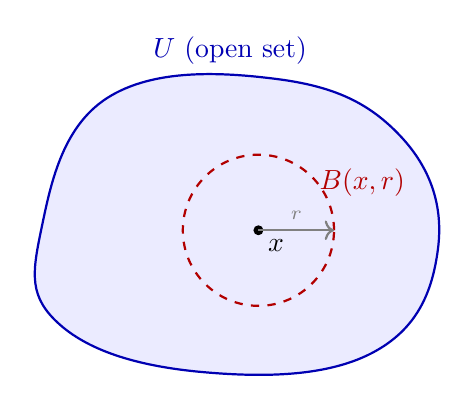
\begin{tikzpicture}[scale=1.2]
  % An open set in R^2 with a ball inside
  \draw[thick, blue!70!black, fill=blue!8]
    plot[smooth cycle, tension=0.7] coordinates
    {(-2,0) (-1.3,1.4) (0.5,1.6) (1.8,1) (2.2,-0.2) (1.5,-1.3) (-0.3,-1.5) (-1.8,-1)};
  \node[blue!70!black] at (0,1.9) {$U$ (open set)};
  % Point x
  \fill (0.3,0) circle (1.5pt) node[below right]{$x$};
  % Ball around x
  \draw[red!70!black, thick, dashed] (0.3,0) circle (0.8);
  \node[red!70!black] at (1.4,0.5) {$B(x,r)$};
  % Arrow
  \draw[->, thick, gray] (0.3,0) -- node[above,font=\scriptsize]{$r$} (1.1,0);
\end{tikzpicture}
\end{center}


%% ──────────────────────────────────────────────────────────
\section{Definition of a topological space}
\label{sec:def-topological-space}

\begin{definition}[Topological space]\label{def:topological-space}
Let $X$ be a non-empty set.  A \textbf{topology}\index{topology} on~$X$ is a
collection $\Tau\subseteq\Pow(X)$ satisfying
\begin{enumerate}[label=\textup{(T\arabic*)}]
  \item\label{ax:T1} $\varnothing\in\Tau$ and $X\in\Tau$.
  \item\label{ax:T2} If $(U_i)_{i\in I}$ is any family of elements of $\Tau$
        (with $I$ an arbitrary index set), then
        $\displaystyle\bigcup_{i\in I}U_i\in\Tau$.
  \item\label{ax:T3} If $U_1,U_2,\ldots,U_n\in\Tau$ (finitely many), then
        $\displaystyle\bigcap_{k=1}^{n}U_k\in\Tau$.
\end{enumerate}
The pair $(X,\Tau)$ is called a \textbf{topological space}\index{topological space}.
The elements of $\Tau$ are called \textbf{open sets}\index{open set}.
\end{definition}

\begin{remark}
Axiom~\ref{ax:T2} allows the empty union ($I=\varnothing$), which gives
$\varnothing\in\Tau$, and axiom~\ref{ax:T3} allows the empty intersection,
which gives $X\in\Tau$.  Hence axiom~\ref{ax:T1} is in fact redundant; it is
included for clarity.
\end{remark}


%% ──────────────────────────────────────────────────────────
\section{First examples}
\label{sec:first-examples}

\begin{definition}[Discrete topology]\label{def:discrete}
The \textbf{discrete topology}\index{topology!discrete}\index{discrete topology}
on a set $X$ is $\Tau_{\mathrm{disc}}=\Pow(X)$, the collection of \emph{all}
subsets of~$X$.
\end{definition}

\begin{definition}[Indiscrete (trivial) topology]\label{def:indiscrete}
The \textbf{indiscrete topology}\index{topology!indiscrete}\index{indiscrete topology}
on a set $X$ is $\Tau_{\mathrm{ind}}=\{\varnothing,\,X\}$.
\end{definition}

\begin{remark}
The discrete topology is the finest possible topology on~$X$, and the
indiscrete topology is the coarsest.  In the discrete topology \emph{every}
subset is open (and closed); in the indiscrete topology the only open sets are
$\varnothing$ and~$X$.
\end{remark}

\begin{definition}[Cofinite topology]\label{def:cofinite}
The \textbf{cofinite topology}\index{topology!cofinite}\index{cofinite topology}
on a set $X$ is
\[
  \Tau_{\mathrm{cof}}
  \;=\;
  \{\, U\subseteq X : X\setminus U \text{ is finite}\,\}
  \;\cup\;
  \{\varnothing\}.
\]
\end{definition}

\begin{proposition}\label{prop:cofinite-is-topology}
The cofinite topology is indeed a topology.
\end{proposition}
\begin{proof}
We verify the three axioms.
\begin{enumerate}[label=(\roman*)]
  \item $\varnothing\in\Tau_{\mathrm{cof}}$ by definition.
        $X\in\Tau_{\mathrm{cof}}$ because $X\setminus X=\varnothing$ is finite.
  \item Let $(U_i)_{i\in I}$ be a family in $\Tau_{\mathrm{cof}}$.
        If every $U_i=\varnothing$ the union is $\varnothing\in\Tau_{\mathrm{cof}}$.
        Otherwise, pick some $j\in I$ with $U_j\neq\varnothing$.  Then
        \[
          X\setminus\bigcup_{i\in I}U_i
          \;=\;\bigcap_{i\in I}(X\setminus U_i)
          \;\subseteq\; X\setminus U_j,
        \]
        which is finite.  So the union is in $\Tau_{\mathrm{cof}}$.
  \item Let $U_1,\ldots,U_n\in\Tau_{\mathrm{cof}}$.  If some $U_k=\varnothing$
        the intersection is $\varnothing\in\Tau_{\mathrm{cof}}$.  Otherwise,
        \[
          X\setminus\bigcap_{k=1}^{n}U_k
          \;=\;\bigcup_{k=1}^{n}(X\setminus U_k),
        \]
        which is a finite union of finite sets, hence finite.  \qedhere
\end{enumerate}
\end{proof}

\begin{definition}[Cocountable topology]\label{def:cocountable}
The \textbf{cocountable topology}\index{topology!cocountable}\index{cocountable topology}
on a set $X$ is
\[
  \Tau_{\mathrm{coc}}
  \;=\;
  \{\, U\subseteq X : X\setminus U \text{ is countable}\,\}
  \;\cup\;
  \{\varnothing\}.
\]
\end{definition}

\begin{remark}
The verification that $\Tau_{\mathrm{coc}}$ is a topology proceeds exactly as
for the cofinite topology, replacing ``finite'' by ``countable'' throughout.
\end{remark}

\begin{exampleplain}[The metric topology]\label{ex:metric-topology}
\index{topology!metric}\index{metric topology}
Let $(X,d)$ be a metric space.  The collection
\[
  \Tau_d \;=\; \{\, U\subseteq X : \forall\, x\in U,\;\exists\, r>0,\;
                  B(x,r)\subseteq U\,\}
\]
is a topology on~$X$, called the \textbf{metric topology} induced by~$d$.
Classical examples include
\begin{itemize}
  \item $\R$ with the Euclidean metric $d(x,y)=|x-y|$, giving the
        \textbf{standard topology}\index{standard topology on $\R$} on~$\R$.
  \item $\R^n$ with $d(\mathbf{x},\mathbf{y})=\|\mathbf{x}-\mathbf{y}\|_2$.
  \item Any normed vector space $(V,\|\cdot\|)$ with $d(x,y)=\|x-y\|$.
\end{itemize}
\end{exampleplain}

\begin{exampleplain}[The Zariski topology on $\R$ --- a brief preview]
\label{ex:zariski-preview}
\index{Zariski topology}
Let $X=\R$ (or more generally an algebraically closed field~$k$).  Declare a
subset $C\subseteq\R$ to be \emph{closed} if it is the zero set of some
collection of polynomials.  Since a non-zero polynomial in one variable has
only finitely many roots, the closed sets in this topology on~$\R$ are
precisely the finite sets and~$\R$ itself.  In other words the Zariski topology
on~$\R$ coincides with the cofinite topology.  In higher dimensions (on~$k^n$
or on algebraic varieties) the Zariski topology is far richer and plays a
central role in algebraic geometry.
\end{exampleplain}


%% ──────────────────────────────────────────────────────────
\section{Comparing topologies}
\label{sec:comparing-topologies}

\begin{definition}[Finer and coarser topologies]\label{def:finer-coarser}
\index{finer topology}\index{coarser topology}
Let $\Tau_1$ and $\Tau_2$ be two topologies on the same set~$X$.  We say that
$\Tau_2$ is \textbf{finer} (or \textbf{stronger}) than $\Tau_1$, and $\Tau_1$
is \textbf{coarser} (or \textbf{weaker}) than $\Tau_2$, if
$\Tau_1\subseteq\Tau_2$.
\end{definition}

\begin{remark}
The relation $\Tau_1\subseteq\Tau_2$ is a partial order on the set of all
topologies on~$X$.  In this partial order the indiscrete topology
$\{\varnothing,X\}$ is the minimum and the discrete topology $\Pow(X)$ is the
maximum.
\end{remark}

\begin{exampleplain}[Lattice of topologies on a three-element set]
\label{ex:lattice-three}
Let $X=\{a,b,c\}$.  The following diagram shows several topologies on~$X$,
ordered by inclusion (lines go upward toward finer topologies):
\begin{center}
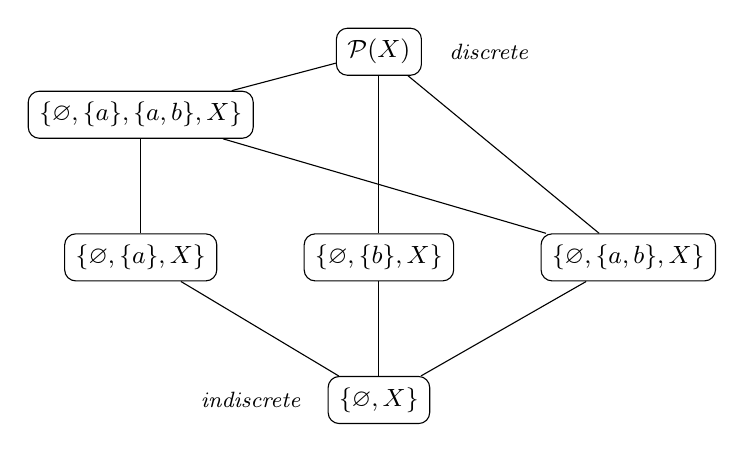
\begin{tikzpicture}[
    node distance=1.4cm,
    every node/.style={draw, rounded corners, inner sep=4pt, font=\small}
  ]
  \node (bot) {$\{\varnothing,X\}$};
  \node (t1) [above left=1.2cm and 1.4cm of bot]
    {$\{\varnothing,\{a\},X\}$};
  \node (t2) [above=1.2cm of bot]
    {$\{\varnothing,\{b\},X\}$};
  \node (t3) [above right=1.2cm and 1.4cm of bot]
    {$\{\varnothing,\{a,b\},X\}$};
  \node (t4) [above=1.2cm of t1]
    {$\{\varnothing,\{a\},\{a,b\},X\}$};
  \node (top) [above=2cm of t2] {$\Pow(X)$};
  \draw (bot)--(t1); \draw (bot)--(t2); \draw (bot)--(t3);
  \draw (t1)--(t4); \draw (t3)--(t4);
  \draw (t4)--(top); \draw (t2)--(top); \draw (t3)--(top);
  % Labels
  \node[draw=none, left=0.2cm of bot, font=\footnotesize\itshape] {indiscrete};
  \node[draw=none, right=0.2cm of top, font=\footnotesize\itshape] {discrete};
\end{tikzpicture}
\end{center}
(Only a selection of the 29 topologies on a 3-element set is shown.)
\end{exampleplain}

\begin{proposition}[Intersection of topologies]
\label{prop:intersection-topologies}
\index{intersection of topologies}
Let $(\Tau_i)_{i\in I}$ be a family of topologies on a set~$X$.  Then
\[
  \Tau \;=\; \bigcap_{i\in I}\Tau_i
\]
is a topology on~$X$.
\end{proposition}

\begin{proof}
We check the three axioms.
\begin{enumerate}[label=(\roman*)]
  \item Since $\varnothing\in\Tau_i$ and $X\in\Tau_i$ for every $i\in I$,
        we have $\varnothing,X\in\Tau$.
  \item Let $(U_j)_{j\in J}$ be a family of elements of~$\Tau$.  For each
        $j\in J$ and each $i\in I$ we have $U_j\in\Tau_i$.  Because each
        $\Tau_i$ is a topology, $\bigcup_{j\in J}U_j\in\Tau_i$.  This holds
        for every~$i$, so $\bigcup_{j\in J}U_j\in\Tau$.
  \item Similarly, if $U_1,\ldots,U_n\in\Tau$ then
        $\bigcap_{k=1}^{n}U_k\in\Tau_i$ for every $i\in I$, hence
        $\bigcap_{k=1}^{n}U_k\in\Tau$.  \qedhere
\end{enumerate}
\end{proof}

\begin{remark}\label{rem:union-not-topology}
The \emph{union} of two topologies need not be a topology.  For instance on
$X=\{a,b,c\}$ let $\Tau_1=\{\varnothing,\{a\},X\}$ and
$\Tau_2=\{\varnothing,\{b\},X\}$.  Then
$\Tau_1\cup\Tau_2=\{\varnothing,\{a\},\{b\},X\}$, which is not closed under
unions since $\{a\}\cup\{b\}=\{a,b\}\notin\Tau_1\cup\Tau_2$.
\end{remark}


%% ──────────────────────────────────────────────────────────
\section{Neighborhoods}
\label{sec:neighborhoods}

\begin{definition}[Neighborhood]\label{def:neighborhood}
\index{neighborhood}
Let $(X,\Tau)$ be a topological space and $x\in X$.  A subset $V\subseteq X$
is a \textbf{neighborhood} of~$x$ if there exists an open set $U\in\Tau$ with
$x\in U\subseteq V$.  The collection of all neighborhoods of~$x$ is denoted
$\Nbhd(x)$ and is called the \textbf{neighborhood system}%
\index{neighborhood system} (or \textbf{neighborhood filter}) of~$x$.
\end{definition}

\begin{remark}
Note that a neighborhood of $x$ is \emph{not} required to be open; it merely
needs to \emph{contain} an open set around~$x$.  An open set $U$ is a
neighborhood of each of its points.
\end{remark}

\begin{proposition}\label{prop:neighborhood-properties}
Let $(X,\Tau)$ be a topological space and $x\in X$.  The neighborhood system
$\Nbhd(x)$ satisfies
\begin{enumerate}[label=\textup{(N\arabic*)}]
  \item\label{N1} $\Nbhd(x)\neq\varnothing$, and every $V\in\Nbhd(x)$
        contains~$x$.
  \item\label{N2} If $V\in\Nbhd(x)$ and $V\subseteq W\subseteq X$, then
        $W\in\Nbhd(x)$.
  \item\label{N3} If $V_1,V_2\in\Nbhd(x)$ then $V_1\cap V_2\in\Nbhd(x)$.
  \item\label{N4} For every $V\in\Nbhd(x)$ there exists $W\in\Nbhd(x)$ with
        $W\subseteq V$ such that $V\in\Nbhd(y)$ for all $y\in W$.
\end{enumerate}
\end{proposition}
\begin{proof}
\ref{N1}: $X$ is open and $x\in X$, so $X\in\Nbhd(x)$.  By definition every
neighborhood contains~$x$.

\ref{N2}: There exists an open $U$ with $x\in U\subseteq V\subseteq W$, so $W$
is a neighborhood of~$x$.

\ref{N3}: There exist open sets $U_1,U_2$ with $x\in U_1\subseteq V_1$ and
$x\in U_2\subseteq V_2$.  Then $U_1\cap U_2$ is open (finite intersection) and
$x\in U_1\cap U_2\subseteq V_1\cap V_2$.

\ref{N4}: Let $V\in\Nbhd(x)$ and pick an open $U$ with $x\in U\subseteq V$.
Set $W=U$.  For every $y\in W=U$, we have $y\in U\subseteq V$ with $U$ open,
so $V\in\Nbhd(y)$.
\end{proof}

\begin{proposition}[Characterization of open sets via neighborhoods]
\label{prop:open-iff-nbhd}
\index{open set!characterization via neighborhoods}
Let $(X,\Tau)$ be a topological space and $U\subseteq X$.  Then $U$ is open
if and only if $U$ is a neighborhood of each of its points; that is,
\[
  U\in\Tau
  \quad\Longleftrightarrow\quad
  \forall\, x\in U,\; U\in\Nbhd(x).
\]
\end{proposition}

\begin{proof}
$(\Rightarrow)$\; If $U$ is open and $x\in U$, then $x\in U\subseteq U$ with
$U$ open, so $U\in\Nbhd(x)$.

$(\Leftarrow)$\; Suppose that for every $x\in U$ there exists an open set
$U_x$ with $x\in U_x\subseteq U$.  Then
\[
  U \;=\; \bigcup_{x\in U} U_x.
\]
As an arbitrary union of open sets, $U$ is open.
\end{proof}


%% ──────────────────────────────────────────────────────────
\section{Why finite intersections?  A counterexample}
\label{sec:counterexample-infinite-intersection}

\begin{exampleplain}[Arbitrary intersections of open sets need not be open]
\label{ex:infinite-intersection-not-open}
\index{intersection!infinite, of open sets}
In $\R$ with the standard topology, consider the open intervals
$U_n=(-1/n,\,1/n)$ for $n\geq 1$.  Each $U_n$ is open.  However,
\[
  \bigcap_{n=1}^{\infty}U_n \;=\; \{0\},
\]
which is \emph{not} open in~$\R$ (no open interval is contained in a single
point).  This is why axiom~\ref{ax:T3} requires only \emph{finite}
intersections.
\end{exampleplain}

\begin{center}
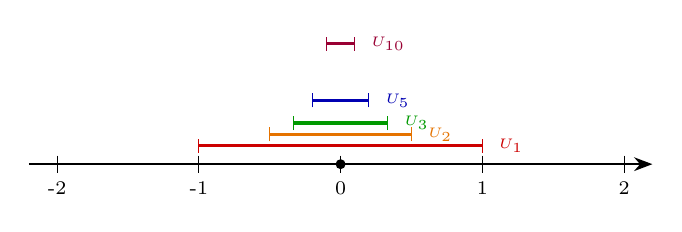
\begin{tikzpicture}[>=Stealth, scale=1.8]
  % Number line
  \draw[thick,->] (-2.2,0) -- (2.2,0);
  \foreach \x in {-2,-1,0,1,2}
    \draw (\x,0.06)--(\x,-0.06) node[below,font=\scriptsize]{\x};
  % Intervals
  \foreach \n/\c in {1/red!80!black, 2/orange!90!black, 3/green!60!black,
                     5/blue!70!black, 10/purple!80!black} {
    \pgfmathsetmacro{\r}{1/\n}
    \draw[\c, very thick] ({-\r},0.08*\n+0.05) -- ({\r},0.08*\n+0.05);
    \draw[\c] ({-\r},0.08*\n) -- ({-\r},0.08*\n+0.1);
    \draw[\c] ({\r},0.08*\n) -- ({\r},0.08*\n+0.1);
    \node[\c,font=\tiny,right] at ({\r+0.05},0.08*\n+0.05) {$U_{\n}$};
  }
  \fill (0,0) circle (1pt);
\end{tikzpicture}
\end{center}


%% ──────────────────────────────────────────────────────────
\section{Worked examples}
\label{sec:worked-examples-ch1}

\begin{exampleplain}[Worked Example 1: verifying a topology]
\label{ex:worked1}
Let $X=\{1,2,3,4\}$ and $\Tau=\{\varnothing,\{1\},\{1,2\},\{1,2,3\},X\}$.
Is $(X,\Tau)$ a topological space?

\emph{Solution.}  We check the axioms.
\begin{itemize}
  \item (T1): $\varnothing,X\in\Tau$. \checkmark
  \item (T2, unions): List all possible unions of elements of~$\Tau$.  Since
        $\Tau$ is a chain $\varnothing\subseteq\{1\}\subseteq\{1,2\}
        \subseteq\{1,2,3\}\subseteq X$, any union of elements is the largest
        element in the union, which is again in $\Tau$. \checkmark
  \item (T3, finite intersections): Similarly, any finite intersection is the
        smallest element, which is in~$\Tau$. \checkmark
\end{itemize}
Hence $(X,\Tau)$ is a topological space.
\end{exampleplain}

\begin{exampleplain}[Worked Example 2: the cofinite topology on $\Z$]
\label{ex:worked2}
In $(\Z,\Tau_{\mathrm{cof}})$, determine whether $A=\{0,1,2\}$ is open,
closed, both, or neither.

\emph{Solution.}
\begin{itemize}
  \item \emph{Open?}  $\Z\setminus A = \Z\setminus\{0,1,2\}$ is infinite
        (it contains all integers outside $\{0,1,2\}$).  So $A$ is
        \textbf{not open}.
  \item \emph{Closed?}  A set is closed if its complement is open.
        $A^c=\Z\setminus\{0,1,2\}$ is not open (since $\Z\setminus A^c=A$ is
        finite).  Wait --- let us recheck: $\Z\setminus(\Z\setminus A)=A$,
        which \emph{is} finite.  So $\Z\setminus A$ \emph{is} open in the
        cofinite topology, meaning $A$ \textbf{is closed}.
\end{itemize}
Therefore $A=\{0,1,2\}$ is closed but not open in $(\Z,\Tau_{\mathrm{cof}})$.
This illustrates that in the cofinite topology on an infinite set, the finite
non-empty subsets are closed but not open.
\end{exampleplain}

\begin{exampleplain}[Worked Example 3: neighborhood systems]
\label{ex:worked3}
Let $X=\{a,b,c\}$ and $\Tau=\{\varnothing,\{a\},\{a,b\},X\}$.  Determine
$\Nbhd(a)$, $\Nbhd(b)$, and $\Nbhd(c)$.

\emph{Solution.}
A set $V$ is a neighborhood of $x$ if there exists $U\in\Tau$ with
$x\in U\subseteq V$.

\begin{itemize}
  \item $\Nbhd(a)$: The open sets containing $a$ are $\{a\}$, $\{a,b\}$,
        and $X$.  Every superset of $\{a\}$ is a neighborhood of~$a$.  Hence
        \[
          \Nbhd(a) = \{\{a\},\,\{a,b\},\,\{a,c\},\,\{a,b,c\}\}.
        \]
  \item $\Nbhd(b)$: The open sets containing $b$ are $\{a,b\}$ and $X$.
        Every superset of $\{a,b\}$ is a neighborhood of~$b$.  Hence
        \[
          \Nbhd(b) = \{\{a,b\},\,\{a,b,c\}\} = \{\{a,b\},\, X\}.
        \]
  \item $\Nbhd(c)$: The only open set containing $c$ is $X$.  Hence
        $\Nbhd(c)=\{X\}$.
\end{itemize}
Notice that the point~$c$ is ``barely visible'' to the topology: the only way
to ``surround'' it with an open set is to take the entire space.
\end{exampleplain}


%% ──────────────────────────────────────────────────────────
\section{Exercises}
\label{sec:exercises-ch1}

\begin{exercise}[$\bigstar$]
\label{exer:ch1:1}
Let $X=\{1,2,3\}$.  List \emph{all} topologies on~$X$ that contain the set
$\{1,2\}$.
\end{exercise}

\begin{exercise}[$\bigstar$]
\label{exer:ch1:2}
Show that on any set~$X$, the discrete topology is the only topology in which
every singleton $\{x\}$ is open.
\end{exercise}

\begin{exercise}[$\bigstar$]
\label{exer:ch1:3}
Let $(X,d)$ be a metric space.  Prove directly (using the triangle inequality)
that every open ball $B(x,r)$ is an open set in the metric topology~$\Tau_d$.
\end{exercise}

\begin{exercise}[$\bigstar\!\bigstar$]
\label{exer:ch1:4}
On $\R$, consider the collection
\[
  \Tau_{[-\infty)} = \{(-\infty,a) : a\in\R\}\cup\{\varnothing,\R\}.
\]
Prove that $\Tau_{[-\infty)}$ is a topology on~$\R$.  Is it finer or coarser
than the standard topology?
\end{exercise}

\begin{exercise}[$\bigstar\!\bigstar$]
\label{exer:ch1:5}
\index{particular point topology}
Let $X$ be a set and $p\in X$ a fixed point.  Define
\[
  \Tau_p = \{\varnothing\}\cup\{U\subseteq X : p\in U\}.
\]
\begin{enumerate}[label=(\alph*)]
  \item Prove that $\Tau_p$ is a topology on~$X$ (the \emph{particular point
        topology}).
  \item Determine the neighborhood system $\Nbhd(p)$ and $\Nbhd(x)$ for
        $x\neq p$.
  \item Is $(X,\Tau_p)$ metrizable when $|X|\geq 2$?  (Hint: consider the $T_1$
        axiom.)
\end{enumerate}
\end{exercise}

\begin{exercise}[$\bigstar\!\bigstar$]
\label{exer:ch1:6}
Let $f\colon X\to Y$ be a function and let $\Tau_Y$ be a topology on~$Y$.
Show that
\[
  \Tau_f = \{f^{-1}(V) : V\in\Tau_Y\}
\]
is a topology on~$X$ (the \emph{initial topology} or \emph{pullback topology}
induced by~$f$).
\end{exercise}

\begin{exercise}[$\bigstar\!\bigstar\!\bigstar$]
\label{exer:ch1:7}
Prove that the set of all topologies on a set~$X$, ordered by inclusion, forms
a \textbf{complete lattice}: every non-empty family of topologies has a
greatest lower bound (infimum) and a least upper bound (supremum).
\begin{enumerate}[label=(\alph*)]
  \item Show that the infimum of a family $(\Tau_i)_{i\in I}$ is
        $\bigcap_{i\in I}\Tau_i$.
  \item Show that the supremum is the coarsest topology containing
        $\bigcup_{i\in I}\Tau_i$ (describe it explicitly).
\end{enumerate}
\end{exercise}

\begin{exercise}[$\bigstar\!\bigstar\!\bigstar$]
\label{exer:ch1:8}
Let $X$ be an infinite set.  Prove that the cofinite topology $\Tau_{\mathrm{cof}}$
on~$X$ is \textbf{not} metrizable.
\emph{Hint:} Suppose $\Tau_{\mathrm{cof}}=\Tau_d$ for some metric~$d$.  Show
that distinct points can be separated by disjoint open sets in~$\Tau_d$
(Hausdorff property), then derive a contradiction with the cofinite topology.
\end{exercise}

\begin{exercise}[$\bigstar$]
\label{exer:ch1:9}
In $\R$ with the standard topology, give an example of a collection of open
sets whose intersection is:
\begin{enumerate}[label=(\alph*)]
  \item open,
  \item closed but not open,
  \item neither open nor closed.
\end{enumerate}
\end{exercise}


%% ──────────────────────────────────────────────────────────
\section*{Chapter summary}
\addcontentsline{toc}{section}{Chapter summary}

\begin{itemize}
  \item A \textbf{topology} on a set $X$ is a collection $\Tau\subseteq\Pow(X)$
        that is closed under arbitrary unions and finite intersections and
        contains both $\varnothing$ and~$X$.
  \item Key examples include the \textbf{discrete}, \textbf{indiscrete},
        \textbf{cofinite}, \textbf{cocountable}, and \textbf{metric}
        topologies.
  \item Topologies on~$X$ are partially ordered by inclusion (\textbf{finer} vs.\
        \textbf{coarser}).  The intersection of any family of topologies is
        again a topology; the union need not be.
  \item A \textbf{neighborhood} of~$x$ is any set containing an open set
        around~$x$.  A set is open if and only if it is a neighborhood of each
        of its points.
  \item Arbitrary intersections of open sets need not be open: the
        finiteness condition in axiom (T3) is essential.
\end{itemize}


%%%%%%%%%%%%%%%%%%%%%%%%%%%%%%%%%%%%%%%%%%%%%%%%%%%%%%%%%%%%
%%
%%  CHAPTER 2
%%
%%%%%%%%%%%%%%%%%%%%%%%%%%%%%%%%%%%%%%%%%%%%%%%%%%%%%%%%%%%%
\chapter{Open Sets, Closed Sets, Interior, Closure, Boundary}
\label{chap:open-closed-interior-closure}

\section*{Motivation: beyond $\varepsilon$-balls}
\addcontentsline{toc}{section}{Motivation: beyond $\varepsilon$-balls}

In a metric space $(X,d)$, one says that a point $x$ is in the \emph{interior}
of a set~$A$ if some $\varepsilon$-ball around~$x$ lies entirely within~$A$,
and that $x$ belongs to the \emph{closure} of~$A$ if every $\varepsilon$-ball
around~$x$ meets~$A$.  The \emph{boundary} consists of those points whose
every $\varepsilon$-ball meets both $A$ and its complement.

These notions extend verbatim to topological spaces: one simply replaces
``$\varepsilon$-ball'' by ``open neighborhood.''  This chapter develops the
theory of interior, closure, boundary, and the related notions of dense and
nowhere dense sets.  A highlight is Kuratowski's elegant axiomatization of
topology via a closure operator, and the remarkable ``14-set theorem.''


%% ──────────────────────────────────────────────────────────
\section{Closed sets}
\label{sec:closed-sets}

\begin{definition}[Closed set]\label{def:closed-set}
\index{closed set}
Let $(X,\Tau)$ be a topological space.  A subset $F\subseteq X$ is
\textbf{closed} if its complement $X\setminus F$ is open, i.e.,
$X\setminus F\in\Tau$.
\end{definition}

\begin{proposition}\label{prop:closed-set-properties}
The collection of closed subsets of a topological space $(X,\Tau)$ satisfies
\begin{enumerate}[label=\textup{(C\arabic*)}]
  \item\label{C1} $\varnothing$ and $X$ are closed.
  \item\label{C2} Any \emph{intersection} of closed sets is closed.
  \item\label{C3} Any \emph{finite union} of closed sets is closed.
\end{enumerate}
\end{proposition}

\begin{proof}
These follow from the axioms for open sets via De Morgan's laws.
\begin{enumerate}[label=(\roman*)]
  \item $X\setminus\varnothing=X\in\Tau$ and $X\setminus X=\varnothing\in\Tau$.
  \item If $(F_i)_{i\in I}$ are closed, then each $X\setminus F_i$ is open,
        and
        $X\setminus\bigcap_{i\in I}F_i=\bigcup_{i\in I}(X\setminus F_i)\in\Tau$.
  \item If $F_1,\ldots,F_n$ are closed, then
        $X\setminus\bigcup_{k=1}^{n}F_k=\bigcap_{k=1}^{n}(X\setminus F_k)\in\Tau$.
        \qedhere
\end{enumerate}
\end{proof}

\begin{remark}
``Open'' and ``closed'' are \emph{not} mutually exclusive.  The empty set and
the whole space~$X$ are always both open and closed (\textbf{clopen}%
\index{clopen set}).  In the discrete topology every set is clopen.  A set may
also be neither open nor closed; for instance $[0,1)$ in~$\R$ with the standard
topology.
\end{remark}


%% ──────────────────────────────────────────────────────────
\section{Interior of a set}
\label{sec:interior}

\begin{definition}[Interior]\label{def:interior}
\index{interior}
Let $(X,\Tau)$ be a topological space and $A\subseteq X$.  The
\textbf{interior} of~$A$, denoted $\interior{A}$, $A^\circ$, or $\Int(A)$, is
\[
  \Int(A) \;=\; \bigcup\{U\in\Tau : U\subseteq A\}.
\]
\end{definition}

\begin{proposition}[Characterizations and properties of the interior]
\label{prop:interior-properties}
Let $(X,\Tau)$ be a topological space and $A,B\subseteq X$.
\begin{enumerate}[label=\textup{(\roman*)}]
  \item\label{int:largest-open}
        $\Int(A)$ is the \textbf{largest open set} contained in~$A$.
  \item\label{int:open-iff}
        $A$ is open if and only if $A=\Int(A)$.
  \item\label{int:membership}
        $x\in\Int(A)$ if and only if $A$ is a neighborhood of~$x$ (i.e.,
        $A\in\Nbhd(x)$).
  \item\label{int:monotone}
        If $A\subseteq B$ then $\Int(A)\subseteq\Int(B)$.
  \item\label{int:idempotent}
        $\Int(\Int(A))=\Int(A)$.
  \item\label{int:intersection}
        $\Int(A\cap B)=\Int(A)\cap\Int(B)$.
  \item\label{int:supset}
        $\Int(A)\cup\Int(B)\subseteq\Int(A\cup B)$, and equality need not
        hold.
\end{enumerate}
\end{proposition}

\begin{proof}
\ref{int:largest-open}: By definition $\Int(A)$ is a union of open subsets of~$A$, so it is
open and contained in~$A$.  If $V$ is any open set with $V\subseteq A$, then
$V$ is one of the sets in the union defining $\Int(A)$, so
$V\subseteq\Int(A)$.

\ref{int:open-iff}: If $A$ is open then $A$ appears in the union
$\Int(A)=\bigcup\{U\in\Tau:U\subseteq A\}$, so $A\subseteq\Int(A)$; the
reverse inclusion is clear.  Conversely, if $A=\Int(A)$ then $A$ is a union of
open sets, hence open.

\ref{int:membership}: $x\in\Int(A)$ iff there exists $U\in\Tau$ with
$x\in U\subseteq A$ iff $A\in\Nbhd(x)$.

\ref{int:monotone}: Every open subset of $A$ is an open subset of $B$.

\ref{int:idempotent}: $\Int(A)$ is open, so $\Int(\Int(A))=\Int(A)$
by~\ref{int:open-iff}.

\ref{int:intersection}: ``$\subseteq$'': $\Int(A)\cap\Int(B)$ is open and
contained in $A\cap B$, hence $\Int(A)\cap\Int(B)\subseteq\Int(A\cap B)$.
``$\supseteq$'': $\Int(A\cap B)\subseteq A\cap B\subseteq A$ and
$\Int(A\cap B)$ is open, so $\Int(A\cap B)\subseteq\Int(A)$.  Similarly
$\Int(A\cap B)\subseteq\Int(B)$.

\ref{int:supset}: $\Int(A)\subseteq A\subseteq A\cup B$ and $\Int(A)$ is open,
so $\Int(A)\subseteq\Int(A\cup B)$; similarly for $\Int(B)$.  For a
counter-example to equality, take $A=\Q$ and $B=\R\setminus\Q$ in $\R$:
$\Int(A)=\Int(B)=\varnothing$ but $\Int(A\cup B)=\Int(\R)=\R$.
\end{proof}


%% ──────────────────────────────────────────────────────────
\section{Closure of a set}
\label{sec:closure}

\begin{definition}[Closure]\label{def:closure}
\index{closure}
Let $(X,\Tau)$ be a topological space and $A\subseteq X$.  The
\textbf{closure} of~$A$, denoted $\cl{A}$ or $\Cl(A)$, is
\[
  \Cl(A) \;=\; \bigcap\{F\subseteq X : F\text{ is closed and }A\subseteq F\}.
\]
\end{definition}

\begin{proposition}[Characterizations and properties of the closure]
\label{prop:closure-properties}
Let $(X,\Tau)$ be a topological space and $A,B\subseteq X$.
\begin{enumerate}[label=\textup{(\roman*)}]
  \item\label{cl:smallest-closed}
        $\Cl(A)$ is the \textbf{smallest closed set} containing~$A$.
  \item\label{cl:closed-iff}
        $A$ is closed if and only if $A=\Cl(A)$.
  \item\label{cl:monotone}
        If $A\subseteq B$ then $\Cl(A)\subseteq\Cl(B)$.
  \item\label{cl:idempotent}
        $\Cl(\Cl(A))=\Cl(A)$.
  \item\label{cl:union}
        $\Cl(A\cup B)=\Cl(A)\cup\Cl(B)$.
  \item\label{cl:intersection}
        $\Cl(A\cap B)\subseteq\Cl(A)\cap\Cl(B)$, and equality need not hold.
  \item\label{cl:complement-int}
        $\Cl(A) = X\setminus\Int(X\setminus A)$ and
        $\Int(A) = X\setminus\Cl(X\setminus A)$.
\end{enumerate}
\end{proposition}

\begin{proof}
The proofs are dual to those of Proposition~\ref{prop:interior-properties}
via complements.  We prove the key identity~\ref{cl:complement-int} and
leave the others as exercises.

\ref{cl:complement-int}: We have
\begin{align*}
  X\setminus\Int(X\setminus A)
  &= X\setminus\bigcup\{U\in\Tau:U\subseteq X\setminus A\} \\
  &= \bigcap\{X\setminus U:U\in\Tau,\;U\subseteq X\setminus A\} \\
  &= \bigcap\{F:F\text{ closed},\; A\subseteq F\}
  = \Cl(A),
\end{align*}
where in the third equality we set $F=X\setminus U$ and note that $U$ ranges
over all open subsets of $X\setminus A$ iff $F=X\setminus U$ ranges over all
closed supersets of~$A$.  The second identity follows by replacing $A$ with
$X\setminus A$.
\end{proof}

\begin{theorem}[Characterization of closure via neighborhoods]
\label{thm:closure-nbhd}
\index{closure!characterization via neighborhoods}
Let $(X,\Tau)$ be a topological space and $A\subseteq X$.  Then
\[
  x\in\Cl(A)
  \quad\Longleftrightarrow\quad
  \text{every open set containing $x$ meets $A$},
\]
i.e., $x\in\Cl(A)$ if and only if $U\cap A\neq\varnothing$ for every
$U\in\Tau$ with $x\in U$.
\end{theorem}

\begin{proof}
We prove both directions by contraposition.

$(\Rightarrow)$ Suppose there exists an open set $U$ with $x\in U$ and
$U\cap A=\varnothing$.  Then $A\subseteq X\setminus U$, and $X\setminus U$ is
closed.  Hence
\[
  \Cl(A) \;\subseteq\; X\setminus U,
\]
and since $x\notin X\setminus U$ we get $x\notin\Cl(A)$.

$(\Leftarrow)$ Suppose $x\notin\Cl(A)$.  Since $\Cl(A)$ is closed,
$U=X\setminus\Cl(A)$ is open.  We have $x\in U$ and
$U\cap A\subseteq U\cap\Cl(A)=\varnothing$, so $U$ is an open neighborhood
of~$x$ that does not meet~$A$.
\end{proof}


%% ──────────────────────────────────────────────────────────
\section{Boundary}
\label{sec:boundary}

\begin{definition}[Boundary]\label{def:boundary}
\index{boundary}
Let $(X,\Tau)$ be a topological space and $A\subseteq X$.  The
\textbf{boundary} (or \textbf{frontier}) of~$A$ is
\[
  \boundary A \;=\; \Cl(A)\setminus\Int(A) \;=\; \Cl(A)\cap\Cl(X\setminus A).
\]
\end{definition}

\begin{proposition}\label{prop:boundary-properties}
Let $(X,\Tau)$ be a topological space and $A\subseteq X$.
\begin{enumerate}[label=\textup{(\roman*)}]
  \item $\boundary A$ is closed.
  \item $\boundary A = \boundary(X\setminus A)$.
  \item $X = \Int(A)\;\sqcup\;\boundary A\;\sqcup\;\Int(X\setminus A)$
        (disjoint union).
  \item $A$ is open if and only if $A\cap\boundary A=\varnothing$.
  \item $A$ is closed if and only if $\boundary A\subseteq A$.
  \item $A$ is clopen if and only if $\boundary A=\varnothing$.
\end{enumerate}
\end{proposition}

\begin{proof}
\begin{enumerate}[label=(\roman*)]
  \item $\boundary A=\Cl(A)\cap\Cl(X\setminus A)$ is the intersection of two
        closed sets.
  \item $\boundary(X\setminus A)=\Cl(X\setminus A)\cap\Cl(A)=\boundary A$.
  \item Every $x\in X$ belongs to exactly one of: $\Int(A)$ (an open
        neighborhood inside~$A$), $\Int(X\setminus A)$ (an open neighborhood
        inside $X\setminus A$), or neither (every open neighborhood
        meets both $A$ and $X\setminus A$, i.e., $x\in\boundary A$).
  \item $A$ is open iff $A=\Int(A)$ iff $A$ contains no boundary points of~$A$
        iff $A\cap\boundary A=\varnothing$.
  \item $A$ is closed iff $\Cl(A)=A$ iff $\boundary A=\Cl(A)\setminus\Int(A)
        \subseteq\Cl(A)=A$.
  \item Combine (iv) and (v).  \qedhere
\end{enumerate}
\end{proof}

%% TikZ diagram: interior, closure, boundary
\begin{center}
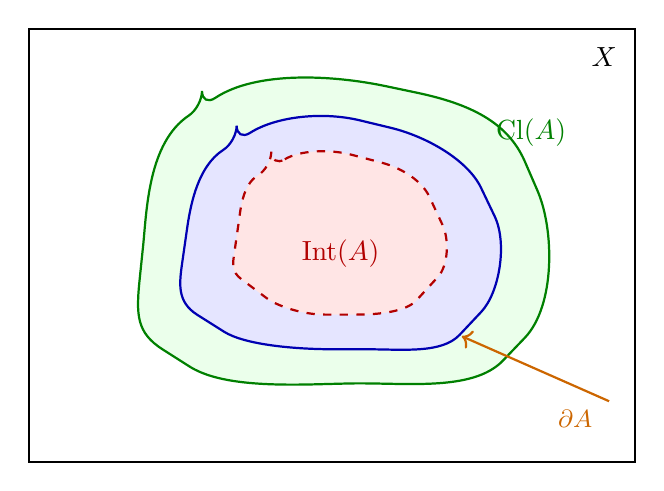
\begin{tikzpicture}[scale=1.1]
  % Ambient space
  \draw[thick] (-3.5,-2.5) rectangle (3.5,2.5);
  \node[anchor=north east] at (3.4,2.4) {$X$};

  % Closure (slightly larger blob)
  \draw[thick, green!50!black, fill=green!8, rounded corners=2mm]
    plot[smooth cycle, tension=0.75] coordinates
    {(-2.2,-0.2) (-1.5,1.6) (0.8,1.8) (2.3,0.8) (2.1,-1.2) (0,-1.6) (-1.8,-1.3)};
  \node[green!50!black] at (2.3,1.3) {$\Cl(A)$};

  % The set A (medium blob)
  \draw[thick, blue!70!black, fill=blue!10, rounded corners=2mm]
    plot[smooth cycle, tension=0.75] coordinates
    {(-1.7,0) (-1.1,1.2) (0.5,1.4) (1.8,0.5) (1.6,-0.9) (0.2,-1.2) (-1.4,-0.9)};
  \node[blue!70!black] at (-0.3,0.3) {$A$};

  % Interior (smaller blob)
  \draw[thick, red!70!black, fill=red!10, rounded corners=2mm, dashed]
    plot[smooth cycle, tension=0.8] coordinates
    {(-1.1,0.1) (-0.7,0.9) (0.4,1) (1.2,0.4) (1.1,-0.5) (0.1,-0.8) (-0.9,-0.5)};
  \node[red!70!black] at (0.1,-0.1) {$\Int(A)$};

  % Labels for boundary
  \draw[->, thick, orange!80!black] (3.2,-1.8) -- (1.5,-1.05);
  \node[orange!80!black, anchor=west, font=\small] at (2.5,-2) {$\boundary A$};
\end{tikzpicture}
\end{center}


%% ──────────────────────────────────────────────────────────
\section{Derived set, limit points, isolated points}
\label{sec:derived-set}

\begin{definition}[Limit point and derived set]\label{def:limit-point}
\index{limit point}\index{derived set}\index{accumulation point|see{limit point}}
Let $(X,\Tau)$ be a topological space and $A\subseteq X$.  A point $x\in X$
is a \textbf{limit point} (or \textbf{accumulation point}) of~$A$ if every
open set containing~$x$ meets $A\setminus\{x\}$:
\[
  \forall\, U\in\Tau,\quad x\in U
  \;\Longrightarrow\; U\cap(A\setminus\{x\})\neq\varnothing.
\]
The set of all limit points of~$A$ is called the \textbf{derived set} of~$A$
and is denoted~$A'$.
\end{definition}

\begin{definition}[Isolated point]\label{def:isolated-point}
\index{isolated point}
A point $a\in A$ is an \textbf{isolated point} of~$A$ if there exists an open
set $U$ such that $U\cap A=\{a\}$.
\end{definition}

\begin{proposition}\label{prop:closure-derived}
For any subset $A$ of a topological space $(X,\Tau)$,
\[
  \Cl(A) = A\cup A'.
\]
\end{proposition}

\begin{proof}
By Theorem~\ref{thm:closure-nbhd}, $x\in\Cl(A)$ iff every open neighborhood
of~$x$ meets~$A$.  If $x\in A$ then $x\in A\cup A'$ trivially.  If
$x\notin A$, then every open neighborhood of~$x$ meeting~$A$ in fact meets
$A\setminus\{x\}=A$, so $x\in A'$.  Hence $\Cl(A)\subseteq A\cup A'$.

Conversely, if $x\in A$ then certainly every open neighborhood meets~$A$
(it contains~$x$), so $x\in\Cl(A)$.  If $x\in A'$ then every open neighborhood
meets $A\setminus\{x\}\subseteq A$, so $x\in\Cl(A)$.
\end{proof}


%% ──────────────────────────────────────────────────────────
\section{Dense sets, nowhere dense sets, and meager sets}
\label{sec:dense-nowhere-dense}

\begin{definition}[Dense set]\label{def:dense}
\index{dense set}
A subset $A$ of a topological space $(X,\Tau)$ is \textbf{dense} in~$X$ if
$\Cl(A)=X$, equivalently, if every non-empty open set meets~$A$.
\end{definition}

\begin{exampleplain}\label{ex:Q-dense}
$\Q$ is dense in $\R$ with the standard topology, because every non-empty open
interval $(a,b)$ contains a rational number (by the Archimedean property).
Similarly, $\R\setminus\Q$ is dense in~$\R$.
\end{exampleplain}

\begin{definition}[Nowhere dense set]\label{def:nowhere-dense}
\index{nowhere dense set}
A subset $A$ of $(X,\Tau)$ is \textbf{nowhere dense} if $\Int(\Cl(A))=\varnothing$;
equivalently, $\Cl(A)$ has empty interior.
\end{definition}

\begin{exampleplain}\label{ex:Z-nowhere-dense}
$\Z$ is nowhere dense in $\R$: $\Cl(\Z)=\Z$ (since $\Z$ is closed in $\R$),
and $\Int(\Z)=\varnothing$ (no open interval is contained in~$\Z$).
\end{exampleplain}

\begin{definition}[Meager set (set of first category)]\label{def:meager}
\index{meager set}\index{first category|see{meager set}}
\index{Baire category}
A subset $M$ of $(X,\Tau)$ is \textbf{meager} (or of \textbf{first category})
if it can be written as a countable union of nowhere dense sets:
\[
  M = \bigcup_{n=1}^{\infty} A_n, \qquad
  \text{each $A_n$ nowhere dense.}
\]
A set that is not meager is said to be of \textbf{second category}.
\end{definition}

\begin{remark}[Preview of Baire's theorem]
The \textbf{Baire category theorem}\index{Baire category theorem} asserts that
in a complete metric space (and more generally in a locally compact Hausdorff
space), the whole space is of second category: it cannot be written as a
countable union of nowhere dense sets.  We shall prove this theorem in a later
chapter.
\end{remark}


%% ──────────────────────────────────────────────────────────
\section{Kuratowski closure axioms}
\label{sec:kuratowski-closure}

Kuratowski observed that a topology on~$X$ can be recovered from its closure
operator.  This gives an equivalent axiomatization of topological spaces.

\begin{theorem}[Kuratowski closure axioms]
\label{thm:kuratowski-axioms}
\index{Kuratowski closure axioms}
Let $X$ be a set and $c\colon\Pow(X)\to\Pow(X)$ an operator satisfying
\begin{enumerate}[label=\textup{(K\arabic*)}]
  \item\label{K1} $c(\varnothing)=\varnothing$.
  \item\label{K2} $A\subseteq c(A)$ for every $A\subseteq X$.
  \item\label{K3} $c(A\cup B)=c(A)\cup c(B)$ for all $A,B\subseteq X$.
  \item\label{K4} $c(c(A))=c(A)$ for every $A\subseteq X$ \textup{(}idempotence\textup{)}.
\end{enumerate}
Then the collection
\[
  \Tau_c \;=\; \{\, U\subseteq X : c(X\setminus U)=X\setminus U\,\}
\]
is a topology on~$X$, and the closure of any set~$A$ in $(X,\Tau_c)$ is
precisely $c(A)$.

Conversely, in any topological space $(X,\Tau)$, the closure operator
$\Cl\colon\Pow(X)\to\Pow(X)$ satisfies \textup{\ref{K1}--\ref{K4}}.
\end{theorem}

\begin{proof}
\textbf{Step 1: $\Tau_c$ is a topology.}

Observe that $U\in\Tau_c$ iff $F=X\setminus U$ satisfies $c(F)=F$; call such
sets \emph{$c$-closed}.

\begin{enumerate}[label=(\roman*)]
  \item $c(X)=c(X\setminus\varnothing)\supseteq X$ by \ref{K2}, so
        $c(X)=X$; thus $X$ is $c$-closed and $\varnothing\in\Tau_c$.
        By \ref{K1}, $\varnothing$ is $c$-closed, so $X\in\Tau_c$.
  \item Let $(F_i)_{i\in I}$ be $c$-closed sets.  We show $F=\bigcap_{i\in I}F_i$
        is $c$-closed.  By \ref{K2}, $F\subseteq c(F)$.  For each $i$,
        $F\subseteq F_i$ so by monotonicity of~$c$
        (which follows from \ref{K2} and \ref{K3}: if $A\subseteq B$ then
        $c(B)=c(A\cup B)=c(A)\cup c(B)\supseteq c(A)$),
        $c(F)\subseteq c(F_i)=F_i$.  Hence $c(F)\subseteq\bigcap_i F_i=F$,
        giving $c(F)=F$.  Thus arbitrary intersections of $c$-closed sets
        are $c$-closed, equivalently, arbitrary unions of sets in $\Tau_c$
        are in~$\Tau_c$.
  \item Let $F_1,F_2$ be $c$-closed.  Then
        $c(F_1\cup F_2)=c(F_1)\cup c(F_2)=F_1\cup F_2$ by \ref{K3},
        so $F_1\cup F_2$ is $c$-closed.  By induction, finite unions of
        $c$-closed sets are $c$-closed, equivalently, finite intersections
        of sets in $\Tau_c$ are in $\Tau_c$.
\end{enumerate}

\textbf{Step 2: The closure in $(X,\Tau_c)$ equals~$c$.}

Let $\Cl_c(A)$ denote the closure of $A$ in $(X,\Tau_c)$.  By definition,
$\Cl_c(A)=\bigcap\{F:F\text{ $c$-closed},\;A\subseteq F\}$.

Since $A\subseteq c(A)$ by \ref{K2} and $c(c(A))=c(A)$ by \ref{K4}, the set
$c(A)$ is $c$-closed and contains~$A$.  Hence $\Cl_c(A)\subseteq c(A)$.

Conversely, if $F$ is $c$-closed and $A\subseteq F$, then
$c(A)\subseteq c(F)=F$.  So $c(A)\subseteq\bigcap\{F:\ldots\}=\Cl_c(A)$.

Therefore $\Cl_c(A)=c(A)$.

\textbf{Step 3: The converse.}

In any topological space $(X,\Tau)$, the closure operator $\Cl$ satisfies
\ref{K1}--\ref{K4} by Proposition~\ref{prop:closure-properties} (items
concerning $\varnothing$, monotonicity, $\Cl(A\cup B)=\Cl(A)\cup\Cl(B)$,
and idempotence).
\end{proof}


%% ──────────────────────────────────────────────────────────
\section{Kuratowski's 14-set theorem}
\label{sec:kuratowski-14}

\begin{theorem}[Kuratowski's 14-set theorem]
\label{thm:kuratowski-14}
\index{Kuratowski's 14-set theorem}
Let $(X,\Tau)$ be a topological space and $A\subseteq X$.  By repeatedly
applying the operations of closure ($\Cl$) and complement ($(\cdot)^c$) to~$A$
in any order, one can obtain \textbf{at most 14} distinct sets.  Moreover,
there exists a set in~$\R$ (with the standard topology) for which all 14 are
distinct.
\end{theorem}

\begin{proof}[Proof sketch]
Denote closure by $k$ and complementation by $c$.  Each of these is a function
$\Pow(X)\to\Pow(X)$.  The key algebraic identities are:
\begin{align}
  c\circ c &= \operatorname{id}, \label{eq:cc}\\
  k\circ k &= k, \label{eq:kk}\\
  k\circ c\circ k\circ c\circ k\circ c\circ k
  &= k\circ c\circ k. \label{eq:kckckck}
\end{align}
Identities~\eqref{eq:cc} and~\eqref{eq:kk} are immediate.  The crucial
identity~\eqref{eq:kckckck} follows from the fact that
$k\circ c\circ k\circ c$ is idempotent (i.e.,
$(k\circ c\circ k\circ c)^2 = k\circ c\circ k\circ c$), which can be proved
using the identity $\Int(\Cl(\Int(\Cl(A))))=\Int(\Cl(A))$ that holds in any
topological space.

Starting from $A$, one generates sets by applying $k$ and $c$ alternately.
Using the three identities above, one can show that the distinct sets obtainable are
at most the following 14:
\begin{center}
\begin{tabular}{rl}
  1. & $A$ \\
  2. & $kA$ \\
  3. & $ckA$ \\
  4. & $kckA$ \\
  5. & $ckckA$ \\
  6. & $kckckA$ \\
  7. & $ckckckA$ \\
  8. & $cA$ \\
  9. & $kcA$ \\
  10. & $ckcA$ \\
  11. & $kckcA$ \\
  12. & $ckckcA$ \\
  13. & $kckckcA$ \\
  14. & $ckckckcA$ \\
\end{tabular}
\end{center}
Any further application of $k$ or $c$ yields one of these 14, by virtue of
\eqref{eq:cc}--\eqref{eq:kckckck}.

\textbf{Sharpness.}  The set
\[
  A = (0,1)\cup(1,2)\cup\{3\}\cup\bigl([4,5]\cap\Q\bigr)
\]
in $\R$ with the standard topology attains all 14 distinct sets.  One verifies
by direct computation:
\begin{itemize}
  \item $A$ has an isolated point ($3$), a ``thick'' part ($[4,5]\cap\Q$ whose
        closure is $[4,5]$ but whose interior is empty), and two intervals
        separated by a point.
  \item Successive applications of closure and complement produce 14 genuinely
        distinct subsets of~$\R$.
\end{itemize}
The verification is elementary but lengthy; we refer the reader to Kuratowski's
original paper (1922) or to Munkres' \emph{Topology}, Problem~2.17.9, for the
full computation.
\end{proof}


%% ──────────────────────────────────────────────────────────
\section{Interior, closure, and boundary in $\R^2$: visualizations}
\label{sec:visualization-R2}

\begin{exampleplain}[The open disk in $\R^2$]
\label{ex:open-disk-R2}
Let $A=\{(x,y)\in\R^2:x^2+y^2<1\}$ be the open unit disk.  Then
$\Int(A)=A$ (it is already open), $\Cl(A)=\{(x,y):x^2+y^2\leq 1\}$ (the
closed disk), and $\boundary A=\{(x,y):x^2+y^2=1\}$ (the unit circle).
\end{exampleplain}

\begin{center}
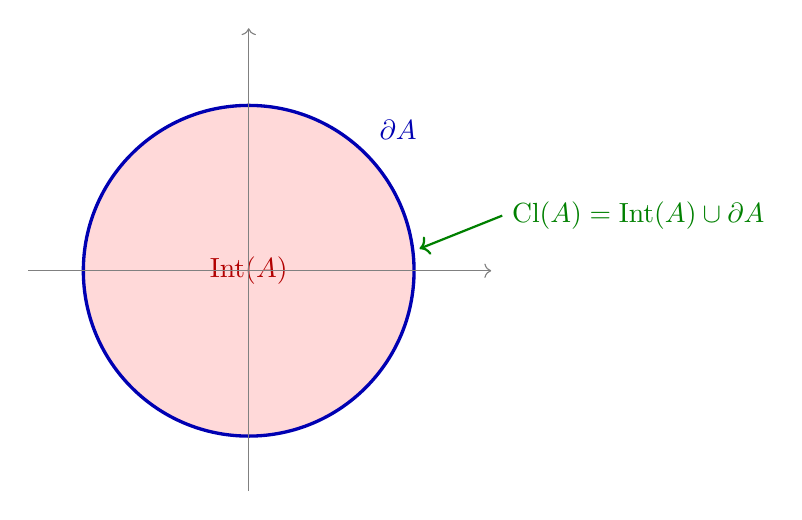
\begin{tikzpicture}[scale=1.4]
  % Interior
  \fill[red!15] (0,0) circle (1.5);
  \node[red!70!black] at (0,0) {$\Int(A)$};
  % Boundary
  \draw[blue!70!black, very thick] (0,0) circle (1.5);
  \node[blue!70!black, anchor=south west] at (1.1,1.1) {$\boundary A$};
  % Closure label
  \draw[->, thick, green!50!black] (2.3,0.5) -- (1.55,0.2);
  \node[green!50!black, anchor=west] at (2.3,0.5) {$\Cl(A)=\Int(A)\cup\boundary A$};
  % Axes
  \draw[thin, gray, ->] (-2,0)--(2.2,0);
  \draw[thin, gray, ->] (0,-2)--(0,2.2);
\end{tikzpicture}
\end{center}

\begin{exampleplain}[A set with non-trivial interior and closure]
\label{ex:half-open-rectangle}
In $\R^2$ consider
$A=[0,1)\times(0,1]$.  Then
\begin{itemize}
  \item $\Int(A)=(0,1)\times(0,1)$,
  \item $\Cl(A)=[0,1]\times[0,1]$,
  \item $\boundary A=\Cl(A)\setminus\Int(A)$, which consists of the four edges
        of the unit square.
\end{itemize}
\end{exampleplain}

\begin{center}
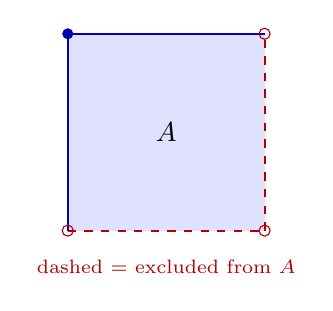
\begin{tikzpicture}[scale=2.5]
  % Filled region (the set A)
  \fill[blue!12] (0,0) rectangle (1,1);
  % Boundary edges: included solid, excluded dashed
  % bottom edge y=0: [0,1)x{0} — excluded (0 not in (0,1])
  \draw[dashed, thick, red!70!black] (0,0) -- (1,0);
  % left edge x=0: {0}x(0,1] — included
  \draw[thick, blue!70!black] (0,0) -- (0,1);
  % top edge y=1: [0,1)x{1} — included
  \draw[thick, blue!70!black] (0,1) -- (1,1);
  % right edge x=1: {1}x(0,1] — excluded
  \draw[dashed, thick, red!70!black] (1,0) -- (1,1);
  % Corner markers
  \fill[blue!70!black] (0,1) circle (0.8pt);
  \draw[red!70!black] (1,0) circle (0.8pt);
  \draw[red!70!black] (1,1) circle (0.8pt);
  \fill[blue!70!black] (0,0) circle (0.0pt);
  \draw[red!70!black] (0,0) circle (0.8pt);
  % Labels
  \node at (0.5,0.5) {$A$};
  \node[anchor=north, font=\scriptsize] at (0.5,-0.1)
    {\color{red!70!black}dashed $=$ excluded from $A$};
\end{tikzpicture}
\end{center}


%% ──────────────────────────────────────────────────────────
\section{Counterexamples and subtleties}
\label{sec:counterexamples-ch2}

\begin{exampleplain}[Sequential closure $\neq$ closure in general]
\label{ex:sequential-closure}
\index{sequential closure}
In a metric space (or more generally a first-countable space), the closure of a
set~$A$ coincides with the \emph{sequential closure}:
\[
  \Cl(A) = \{\, x\in X : \exists\,(x_n)_{n\geq 1}\text{ in }A
            \text{ with }x_n\to x\,\}.
\]
This fails in general topological spaces.  Consider the ordinal space
$X=[0,\omega_1]$ with the order topology, and let
$A=[0,\omega_1)$.  Then $\omega_1\in\Cl(A)$ (every open neighborhood of
$\omega_1$ meets~$A$), but no \emph{sequence} in $A$ converges to~$\omega_1$
(since $\omega_1$ has uncountable cofinality).  Thus the sequential closure of
$A$ is $A$ itself, which is strictly smaller than $\Cl(A)=X$.
\end{exampleplain}

\begin{exampleplain}[$\Q$ is dense in $\R$ but not in the Sorgenfrey line]
\label{ex:sorgenfrey-density}
\index{Sorgenfrey line}
The \textbf{Sorgenfrey line} (or \textbf{lower limit topology}) on $\R$ has
as a basis the half-open intervals $[a,b)$ with $a<b$.  In this topology
$\Q$ is still dense: every non-empty basic open set $[a,b)$ contains a
rational.  However, the Sorgenfrey line is \emph{not} second-countable (it has
no countable basis), and many properties that hold for the standard topology
fail: for instance, the Sorgenfrey line is separable but not second-countable,
showing these two properties are independent outside the metric setting.

More strikingly, consider the set $A=\R\setminus\Q$ of irrationals.  In the
standard topology, $\Cl(A)=\R$ and $\Int(A)=\varnothing$ (the irrationals are
dense with empty interior).  In the Sorgenfrey line the same conclusions hold:
$\Cl(A)=\R$ (every $[a,b)$ contains an irrational) and $\Int(A)=\varnothing$
(no $[a,b)$ is contained in $\R\setminus\Q$, since every such interval
contains rationals).
\end{exampleplain}


%% ──────────────────────────────────────────────────────────
\section{Worked examples}
\label{sec:worked-examples-ch2}

\begin{exampleplain}[Worked Example 1: interior and closure in the cofinite topology]
\label{ex:ch2-worked1}
Let $X=\R$ with the cofinite topology, and let $A=(0,1)$.

\emph{Solution.}
In the cofinite topology, the closed sets are $\R$, $\varnothing$, and all
finite subsets of~$\R$.

\begin{itemize}
  \item \textbf{Closure:} $\Cl(A)$ is the smallest closed set containing~$A$.
        Since $A=(0,1)$ is infinite, the only closed set containing~$A$ is
        $\R$ itself.  Hence $\Cl(A)=\R$.
  \item \textbf{Interior:} $\Int(A)$ is the largest open set contained in~$A$.
        A set $U$ is open in the cofinite topology iff $\R\setminus U$ is
        finite (or $U=\varnothing$).  If $U\subseteq(0,1)$ is open and
        non-empty, then $\R\setminus U$ is finite, but
        $\R\setminus U\supseteq\R\setminus(0,1)=(-\infty,0]\cup[1,\infty)$,
        which is infinite.  Contradiction.  Hence $\Int(A)=\varnothing$.
  \item \textbf{Boundary:} $\boundary A=\Cl(A)\setminus\Int(A)=\R\setminus
        \varnothing=\R$.
\end{itemize}
\end{exampleplain}

\begin{exampleplain}[Worked Example 2: derived set computation]
\label{ex:ch2-worked2}
In $\R$ with the standard topology, let $A=\{1/n:n\in\N,\;n\geq 1\}$.
Find $A'$, $\Cl(A)$, $\Int(A)$, and $\boundary A$.

\emph{Solution.}
\begin{itemize}
  \item \textbf{Limit points ($A'$):}  A point $x$ is a limit point of~$A$ if
        every open neighborhood of~$x$ contains a point of $A$ distinct from~$x$.

        \emph{Claim:} $A'=\{0\}$.  Indeed, every open interval around~$0$
        contains $1/n$ for $n$ sufficiently large, so $0\in A'$.  For
        $x\neq 0$, if $x\notin A$ pick $\varepsilon>0$ smaller than the
        distance from $x$ to the nearest point of $A\cup\{0\}$; then
        $(x-\varepsilon,x+\varepsilon)\cap A=\varnothing$.  If $x=1/n\in A$,
        pick $\varepsilon$ smaller than $\min(1/n-1/(n+1),\,1/(n-1)-1/n)$
        (with the obvious convention for $n=1$); then
        $(x-\varepsilon,x+\varepsilon)\cap(A\setminus\{x\})=\varnothing$.
  \item \textbf{Closure:} $\Cl(A)=A\cup A'=\{0\}\cup\{1/n:n\geq 1\}$.
  \item \textbf{Interior:} $\Int(A)=\varnothing$ (no open interval is
        contained in~$A$, since $A$ is countable).
  \item \textbf{Boundary:} $\boundary A=\Cl(A)\setminus\Int(A)=\Cl(A)
        =\{0,1,1/2,1/3,\ldots\}$.
\end{itemize}
\end{exampleplain}

\begin{exampleplain}[Worked Example 3: the closure of $\Q\times\Q$ in $\R^2$]
\label{ex:ch2-worked3}
In $\R^2$ with the standard (product) topology, let $A=\Q\times\Q$.
Find $\Cl(A)$, $\Int(A)$, and $\boundary A$.

\emph{Solution.}
\begin{itemize}
  \item \textbf{Closure:} Let $(x,y)\in\R^2$ and let $U$ be any open set
        containing $(x,y)$.  Then $U$ contains a product of open intervals
        $(a,b)\times(c,d)$ with $x\in(a,b)$ and $y\in(c,d)$.  Since $\Q$ is
        dense in~$\R$, there exist $q_1\in(a,b)\cap\Q$ and
        $q_2\in(c,d)\cap\Q$, so $(q_1,q_2)\in U\cap A$.  By
        Theorem~\ref{thm:closure-nbhd}, $(x,y)\in\Cl(A)$.  Therefore
        $\Cl(A)=\R^2$.
  \item \textbf{Interior:} If $U\subseteq\Q\times\Q$ were a non-empty open set,
        it would contain a product of open intervals, which contains
        uncountably many points --- but $\Q\times\Q$ is countable.
        Contradiction.  Hence $\Int(A)=\varnothing$.
  \item \textbf{Boundary:} $\boundary A=\Cl(A)\setminus\Int(A)=\R^2$.
\end{itemize}
\end{exampleplain}


%% ──────────────────────────────────────────────────────────
\section{Exercises}
\label{sec:exercises-ch2}

\begin{exercise}[$\bigstar$]
\label{exer:ch2:1}
In $\R$ with the standard topology, find $\Int(A)$, $\Cl(A)$, and
$\boundary A$ for each of the following sets:
\begin{enumerate}[label=(\alph*)]
  \item $A=[0,1)$,
  \item $A=\Q$,
  \item $A=\Z$,
  \item $A=\{1/n:n\in\N,\;n\geq 1\}$.
\end{enumerate}
\end{exercise}

\begin{exercise}[$\bigstar$]
\label{exer:ch2:2}
Prove that a set $A$ is closed if and only if $A'\subseteq A$ (i.e., $A$
contains all its limit points).
\end{exercise}

\begin{exercise}[$\bigstar$]
\label{exer:ch2:3}
Let $(X,\Tau)$ be a topological space.  Prove that $\boundary A=\varnothing$
if and only if $A$ is clopen.
\end{exercise}

\begin{exercise}[$\bigstar\!\bigstar$]
\label{exer:ch2:4}
Let $A$ and $B$ be subsets of a topological space.  Prove or disprove:
\begin{enumerate}[label=(\alph*)]
  \item $\boundary(A\cup B)\subseteq\boundary A\cup\boundary B$.
  \item $\boundary(A\cap B)\subseteq\boundary A\cup\boundary B$.
\end{enumerate}
\end{exercise}

\begin{exercise}[$\bigstar\!\bigstar$]
\label{exer:ch2:5}
Let $A$ be a dense subset of $(X,\Tau)$ and let $U$ be an open set.  Prove
that $\Cl(A\cap U)=\Cl(U)$.
\end{exercise}

\begin{exercise}[$\bigstar\!\bigstar$]
\label{exer:ch2:6}
Verify the Kuratowski closure axioms \textup{(K1)--(K4)} for the closure
operator of the cofinite topology on an infinite set~$X$.
\end{exercise}

\begin{exercise}[$\bigstar\!\bigstar\!\bigstar$]
\label{exer:ch2:7}
\textup{(Kuratowski's 14-set theorem --- explicit computation.)}
Let $A=(0,1)\cup(1,2)\cup\{3\}\cup([4,5]\cap\Q)$ in $\R$ with the standard
topology.  Compute all 14 distinct sets obtained by repeatedly applying
closure and complement to~$A$.
\end{exercise}

\begin{exercise}[$\bigstar\!\bigstar\!\bigstar$]
\label{exer:ch2:8}
Prove that in a topological space $(X,\Tau)$, the following are equivalent:
\begin{enumerate}[label=(\roman*)]
  \item Every subset of $X$ is either open or closed (or both).
  \item The topology $\Tau$ is the discrete topology.
\end{enumerate}
\emph{Hint:} Show that (i) implies every singleton is closed, then that every
singleton is open.
\end{exercise}

\begin{exercise}[$\bigstar\!\bigstar$]
\label{exer:ch2:9}
Let $(X,\Tau)$ be a topological space and $A\subseteq X$.  Prove that
$\Int(A)$, $\boundary A$, and $\Int(X\setminus A)$ form a partition of~$X$
(i.e., they are pairwise disjoint and their union is~$X$).
\end{exercise}

\begin{exercise}[$\bigstar\!\bigstar\!\bigstar$]
\label{exer:ch2:10}
\index{regular open set}
A set $A$ in a topological space is called \textbf{regular open} if
$A=\Int(\Cl(A))$, and \textbf{regular closed} if $A=\Cl(\Int(A))$.
\begin{enumerate}[label=(\alph*)]
  \item Give an example of an open set in $\R$ that is not regular open.
  \item Prove that for any set $A$, $\Int(\Cl(A))$ is regular open.
  \item Prove that the collection of regular open sets of a topological space
        forms a Boolean algebra under the operations $A\wedge B=A\cap B$
        and $A\vee B=\Int(\Cl(A\cup B))$.
\end{enumerate}
\end{exercise}


%% ──────────────────────────────────────────────────────────
\section*{Chapter summary}
\addcontentsline{toc}{section}{Chapter summary}

\begin{itemize}
  \item A set is \textbf{closed} if its complement is open.  Closed sets are
        stable under arbitrary intersections and finite unions.
  \item The \textbf{interior} $\Int(A)$ is the largest open subset of~$A$;
        the \textbf{closure} $\Cl(A)$ is the smallest closed superset
        of~$A$.  They are related by complementation:
        $\Cl(A)=X\setminus\Int(X\setminus A)$.
  \item $x\in\Cl(A)$ if and only if every open neighborhood of~$x$ meets~$A$
        (Theorem~\ref{thm:closure-nbhd}).
  \item The \textbf{boundary} $\boundary A=\Cl(A)\setminus\Int(A)$ consists
        of points every neighborhood of which meets both $A$ and
        $X\setminus A$.
  \item The \textbf{derived set} $A'$ consists of all limit points; one has
        $\Cl(A)=A\cup A'$.
  \item A set is \textbf{dense} if its closure is the whole space;
        \textbf{nowhere dense} if the interior of its closure is empty.
  \item The \textbf{Kuratowski closure axioms} (K1)--(K4) provide an
        equivalent axiomatization of topological spaces via the closure
        operator.
  \item \textbf{Kuratowski's 14-set theorem}: starting from any set,
        repeated application of closure and complement yields at most
        14~distinct sets.
  \item Caution: in non-first-countable spaces, the sequential closure of a
        set may be strictly smaller than the topological closure.
\end{itemize}

%% ══════════════════════════════════════════════════════════
%% END OF PART 1 — Chapters 1 and 2
%% More chapters will be appended below.
%% ══════════════════════════════════════════════════════════
%%%%%%%%%%%%%%%%%%%%%%%%%%%%%%%%%%%%%%%%%%%%%%%%%%%%%%%%%%%%
%% PART 2 — Chapters 3 & 4
%% General Topology (English)
%% Conventions follow Munkres, "Topology" (2nd ed.)
%%%%%%%%%%%%%%%%%%%%%%%%%%%%%%%%%%%%%%%%%%%%%%%%%%%%%%%%%%%%

%==========================================================
% CHAPTER 3 — Bases, Sub-bases, and Generated Topologies
%==========================================================
\chapter{Bases, Sub-bases, and Generated Topologies}
\label{ch:bases}
\index{base|(}
\index{sub-base|(}

In the study of metric spaces one quickly observes that every open set can be
written as a union of open balls.  This single observation carries enormous
organizational power: instead of describing a topology by listing \emph{all} of
its open sets, it suffices to specify a much smaller collection---a
\emph{base}---from which the full topology can be recovered by taking unions.
The notion of a base, and the still more economical notion of a
\emph{sub-base}, are the central themes of this chapter.  They provide
systematic machinery for constructing topologies and for comparing different
topological spaces.

%----------------------------------------------------------
\section{Bases for a topology}
\label{sec:bases-def}

\begin{definition}[Base for a topology]
\label{def:base}
\index{base!for a topology}
Let $(X,\mathscr{T})$ be a topological space.  A collection
$\mathscr{B}\subseteq\mathscr{T}$ is called a \textbf{base} (or
\textbf{basis}) for $\mathscr{T}$ if every open set $U\in\mathscr{T}$ can be
written as a union of members of $\mathscr{B}$; equivalently, for every
$U\in\mathscr{T}$ and every $x\in U$ there exists $B\in\mathscr{B}$ such that
$x\in B\subseteq U$.
\end{definition}

\begin{remark}
\label{rem:base-generates}
If $\mathscr{B}$ is a base for $\mathscr{T}$, then $\mathscr{T}$ equals
the collection of all unions of subfamilies of $\mathscr{B}$ (including the
empty union, which gives $\varnothing$).  We say that $\mathscr{B}$
\emph{generates} $\mathscr{T}$.
\end{remark}

The following criterion tells us exactly when a collection of subsets of a set
$X$ is a base for \emph{some} topology on $X$.

\begin{theorem}[Base criterion]
\label{thm:base-criterion}
\index{base!criterion}
Let $X$ be a set and let $\mathscr{B}$ be a collection of subsets of $X$.
Then $\mathscr{B}$ is a base for some topology on $X$ if and only if the
following two conditions hold:
\begin{enumerate}
    \item[(B1)] $\mathscr{B}$ covers $X$: for every $x\in X$ there exists
        $B\in\mathscr{B}$ with $x\in B$.
    \item[(B2)] For any $B_1,B_2\in\mathscr{B}$ and any $x\in B_1\cap B_2$,
        there exists $B_3\in\mathscr{B}$ such that $x\in B_3\subseteq
        B_1\cap B_2$.
\end{enumerate}
When these conditions hold, the topology $\mathscr{T}_{\mathscr{B}}$ generated
by $\mathscr{B}$ is
\[
    \mathscr{T}_{\mathscr{B}}
    \;=\;
    \bigl\{\, U\subseteq X \;\big|\;
        \forall\, x\in U,\;\exists\, B\in\mathscr{B}:\;
        x\in B\subseteq U
    \bigr\}.
\]
\end{theorem}

\begin{proof}
\textbf{($\Rightarrow$)}
Suppose $\mathscr{B}$ is a base for a topology $\mathscr{T}$ on $X$.  Since
$X\in\mathscr{T}$, every point of $X$ lies in some member of $\mathscr{B}$,
giving~(B1).  For~(B2), let $B_1,B_2\in\mathscr{B}$ and $x\in B_1\cap B_2$.
Because $\mathscr{B}\subseteq\mathscr{T}$ and $\mathscr{T}$ is closed under
finite intersections, $B_1\cap B_2\in\mathscr{T}$.  Since $\mathscr{B}$ is a
base, there exists $B_3\in\mathscr{B}$ with $x\in B_3\subseteq B_1\cap B_2$.

\medskip\noindent
\textbf{($\Leftarrow$)}
Assume (B1) and (B2).  Define
\[
    \mathscr{T}
    \;=\;
    \bigl\{\, U\subseteq X \;\big|\;
        \forall\, x\in U,\;\exists\, B\in\mathscr{B}:\;
        x\in B\subseteq U
    \bigr\}.
\]
We verify the axioms of a topology.

\begin{itemize}
    \item \emph{$\varnothing$ and $X$ belong to $\mathscr{T}$.}\;
        The empty set satisfies the condition vacuously.  By~(B1), every point
        of $X$ lies in some $B\in\mathscr{B}\subseteq\mathscr{P}(X)$, hence
        $X\in\mathscr{T}$.

    \item \emph{Arbitrary unions.}\;
        Let $\{U_\alpha\}_{\alpha\in A}\subseteq\mathscr{T}$ and set
        $U=\bigcup_\alpha U_\alpha$.  If $x\in U$, then $x\in U_\alpha$ for
        some $\alpha$, so there exists $B\in\mathscr{B}$ with
        $x\in B\subseteq U_\alpha\subseteq U$.  Thus $U\in\mathscr{T}$.

    \item \emph{Finite intersections.}\;
        It suffices to treat the intersection of two members.  Let
        $U_1,U_2\in\mathscr{T}$ and $x\in U_1\cap U_2$.  Choose
        $B_1,B_2\in\mathscr{B}$ with $x\in B_1\subseteq U_1$ and
        $x\in B_2\subseteq U_2$.  By~(B2), there exists $B_3\in\mathscr{B}$
        with $x\in B_3\subseteq B_1\cap B_2\subseteq U_1\cap U_2$.  Hence
        $U_1\cap U_2\in\mathscr{T}$.
\end{itemize}

Finally, each $B\in\mathscr{B}$ belongs to $\mathscr{T}$ (take $B_3=B$ for
every $x\in B$), and by construction every member of $\mathscr{T}$ is a union
of members of $\mathscr{B}$.  Therefore $\mathscr{B}$ is a base for
$\mathscr{T}$.
\end{proof}

%----------------------------------------------------------
\section{Sub-bases and generated topologies}
\label{sec:subbases}

\begin{definition}[Sub-base]
\label{def:subbase}
\index{sub-base!definition}
Let $X$ be a set.  A collection $\mathscr{S}$ of subsets of $X$ is called a
\textbf{sub-base} for a topology on $X$ if $\mathscr{S}$ covers $X$, i.e.\
$\bigcup_{S\in\mathscr{S}} S = X$.  The topology \emph{generated} by
$\mathscr{S}$ is the collection $\mathscr{T}_{\mathscr{S}}$ of all unions of
finite intersections of members of $\mathscr{S}$:
\[
    \mathscr{T}_{\mathscr{S}}
    \;=\;
    \Bigl\{\,
        \bigcup_{\alpha\in A}\,
        \bigl(S_{\alpha,1}\cap\cdots\cap S_{\alpha,n_\alpha}\bigr)
        \;\Big|\;
        S_{\alpha,j}\in\mathscr{S}
    \Bigr\}.
\]
Equivalently, the collection
$\mathscr{B}_{\mathscr{S}}=\{S_1\cap\cdots\cap S_n \mid
S_i\in\mathscr{S},\;n\ge 1\}$ is a base for $\mathscr{T}_{\mathscr{S}}$.
\end{definition}

\begin{proposition}
\label{prop:subbase-is-base}
\index{sub-base!generates a base}
Let $\mathscr{S}$ be a sub-base on a set $X$.  Then the collection
$\mathscr{B}_{\mathscr{S}}$ of all finite intersections of members of
$\mathscr{S}$ satisfies conditions \textnormal{(B1)} and \textnormal{(B2)} of
Theorem~\ref{thm:base-criterion} and hence is a base for a topology on~$X$.
\end{proposition}

\begin{proof}
Since $\mathscr{S}$ covers $X$, so does $\mathscr{B}_{\mathscr{S}}$, giving
(B1).  For (B2), if $B_1=\bigcap_{i=1}^{m}S_i$ and
$B_2=\bigcap_{j=1}^{n}T_j$ with $S_i,T_j\in\mathscr{S}$, then
$B_1\cap B_2=\bigcap_{i=1}^{m}S_i\cap\bigcap_{j=1}^{n}T_j$ is itself a
finite intersection of members of $\mathscr{S}$, hence an element of
$\mathscr{B}_{\mathscr{S}}$.  Taking $B_3=B_1\cap B_2$ satisfies~(B2).
\end{proof}

\begin{definition}[Generated topology --- intersection characterization]
\label{def:generated-topology}
\index{generated topology}
Let $\mathscr{A}$ be any collection of subsets of a set $X$.  The
\textbf{topology generated by $\mathscr{A}$} is
\[
    \mathscr{T}(\mathscr{A})
    \;=\;
    \bigcap\bigl\{\,\mathscr{T} \;\big|\;
        \mathscr{T}\text{ is a topology on }X\text{ and }
        \mathscr{A}\subseteq\mathscr{T}
    \bigr\}.
\]
This intersection is nonempty (since the discrete topology contains
$\mathscr{A}$) and is itself a topology on $X$ --- the \emph{smallest}
topology containing every member of $\mathscr{A}$.
\end{definition}

\begin{proposition}
\label{prop:generated-equals-subbase}
If $\mathscr{S}$ covers $X$, then
$\mathscr{T}(\mathscr{S})=\mathscr{T}_{\mathscr{S}}$; that is, the topology
generated by $\mathscr{S}$ in the sense of
Definition~\ref{def:generated-topology} coincides with the sub-base topology of
Definition~\ref{def:subbase}.
\end{proposition}

\begin{proof}
Every topology containing $\mathscr{S}$ must contain all finite intersections
of members of $\mathscr{S}$ and all unions thereof, hence contains
$\mathscr{T}_{\mathscr{S}}$.  Thus
$\mathscr{T}(\mathscr{S})\supseteq\mathscr{T}_{\mathscr{S}}$.  Conversely,
$\mathscr{T}_{\mathscr{S}}$ is a topology containing $\mathscr{S}$ (by
Proposition~\ref{prop:subbase-is-base}), so it is one of the topologies in the
intersection, giving
$\mathscr{T}(\mathscr{S})\subseteq\mathscr{T}_{\mathscr{S}}$.
\end{proof}

%----------------------------------------------------------
\section{Countability and separability axioms}
\label{sec:countability}

\begin{definition}[First and second countability]
\label{def:countability-axioms}
\index{first countable}
\index{second countable}
A topological space $X$ is said to be
\begin{itemize}
    \item \textbf{first countable} if every point $x\in X$ has a countable
        neighborhood base, i.e.\ a countable collection
        $\{B_n\}_{n\in\mathbb{N}}$ of open neighborhoods of $x$ such that for
        every open set $U$ containing $x$ there exists $n$ with
        $B_n\subseteq U$;
    \item \textbf{second countable} if $X$ has a countable base for its
        topology.
\end{itemize}
\end{definition}

\begin{definition}[Separable space]
\label{def:separable}
\index{separable}
A topological space $X$ is \textbf{separable} if it contains a countable dense
subset, i.e.\ a countable set $D\subseteq X$ with $\overline{D}=X$.
\end{definition}

\begin{theorem}[Second countable implies separable]
\label{thm:2nd-countable-separable}
\index{second countable!implies separable}
Every second countable space is separable.
\end{theorem}

\begin{proof}
Let $\mathscr{B}=\{B_n\}_{n\in\mathbb{N}}$ be a countable base for $X$.  For
each $n$ with $B_n\neq\varnothing$, choose a point $x_n\in B_n$ (using the
axiom of countable choice).  Set $D=\{x_n\}$.  Then $D$ is countable.  To see
that $D$ is dense, let $U$ be a nonempty open set.  Since $\mathscr{B}$ is a
base, there exists $B_n\subseteq U$ with $B_n\neq\varnothing$; then
$x_n\in D\cap U$.  Hence every nonempty open set meets $D$, so
$\overline{D}=X$.
\end{proof}

\begin{definition}[Lindel\"{o}f space]
\label{def:lindelof}
\index{Lindelof space@Lindel\"{o}f space}
A topological space $X$ is called a \textbf{Lindel\"{o}f space} if every open
cover of $X$ admits a countable subcover.
\end{definition}

\begin{theorem}[Second countable implies Lindel\"{o}f]
\label{thm:2nd-countable-lindelof}
\index{second countable!implies Lindel\"{o}f}
Every second countable space is a Lindel\"{o}f space.
\end{theorem}

\begin{proof}
Let $\mathscr{B}=\{B_n\}_{n\in\mathbb{N}}$ be a countable base for $X$, and
let $\{U_\alpha\}_{\alpha\in A}$ be an open cover of $X$.  For each $x\in X$
there exist $\alpha_x\in A$ and $B_{n_x}\in\mathscr{B}$ with
$x\in B_{n_x}\subseteq U_{\alpha_x}$.  The collection
$\{B_{n_x}\}_{x\in X}$ is a sub-collection of the countable family
$\mathscr{B}$, so the set of indices $I=\{n_x : x\in X\}\subseteq\mathbb{N}$
is countable.  For each $n\in I$, choose one $\alpha_n\in A$ such that
$B_n\subseteq U_{\alpha_n}$.  Then
$\{U_{\alpha_n}\}_{n\in I}$ is a countable sub-collection of the original
cover, and
\[
    X
    = \bigcup_{x\in X} B_{n_x}
    \subseteq \bigcup_{n\in I} B_n
    \subseteq \bigcup_{n\in I} U_{\alpha_n}
    \subseteq X.
\]
Hence $\{U_{\alpha_n}\}_{n\in I}$ is a countable subcover.
\end{proof}

%----------------------------------------------------------
\section{Standard examples of bases}
\label{sec:base-examples}

\begin{example}[Standard base for $\mathbb{R}$]
\label{ex:base-R}
\index{base!for $\mathbb{R}$}
The collection of all open intervals $(a,b)$ with $a<b$ is a base for the
standard (Euclidean) topology on $\mathbb{R}$.  More economically, the
sub-collection $\{(p,q) : p,q\in\mathbb{Q},\;p<q\}$ is a \emph{countable}
base, showing that $\mathbb{R}$ is second countable.
\end{example}

\begin{example}[Standard base for $\mathbb{R}^n$]
\label{ex:base-Rn}
\index{base!for $\mathbb{R}^n$}
The collection of all open balls $B_d(\mathbf{x},\varepsilon)$ with
$\mathbf{x}\in\mathbb{R}^n$ and $\varepsilon>0$ is a base for the Euclidean
topology.  A countable base is obtained by restricting to rational centers
$\mathbf{x}\in\mathbb{Q}^n$ and rational radii $\varepsilon\in\mathbb{Q}_{>0}$.
Hence $\mathbb{R}^n$ is second countable.
\end{example}

\begin{example}[Sorgenfrey line]
\label{ex:sorgenfrey-base}
\index{Sorgenfrey line!base}
\index{lower limit topology}
The \textbf{Sorgenfrey line} $\mathbb{R}_\ell$ is $\mathbb{R}$ equipped with
the topology generated by the base
$\mathscr{B}=\{[a,b) : a<b,\;a,b\in\mathbb{R}\}$.  One readily checks that
$\mathscr{B}$ satisfies (B1) and (B2).  The resulting topology is strictly
finer than the standard topology.
\end{example}

\begin{example}[Order topology]
\label{ex:order-topology-base}
\index{order topology!base}
Let $(X,\le)$ be a linearly ordered set with more than one element.  The
\textbf{order topology} on $X$ has as a base all sets of the following forms:
\begin{enumerate}
    \item $(a,b)=\{x\in X : a < x < b\}$ for $a<b$ in $X$,
    \item $[a_0,b)=\{x\in X : a_0\le x < b\}$ if $X$ has a smallest element
        $a_0$,
    \item $(a,b_0]=\{x\in X : a < x \le b_0\}$ if $X$ has a largest element
        $b_0$.
\end{enumerate}
\end{example}

%----------------------------------------------------------
\section{Visualizing base elements}
\label{sec:base-tikz}

The following diagram illustrates how an open set $U$ is expressed as a union
of base elements.

\begin{center}
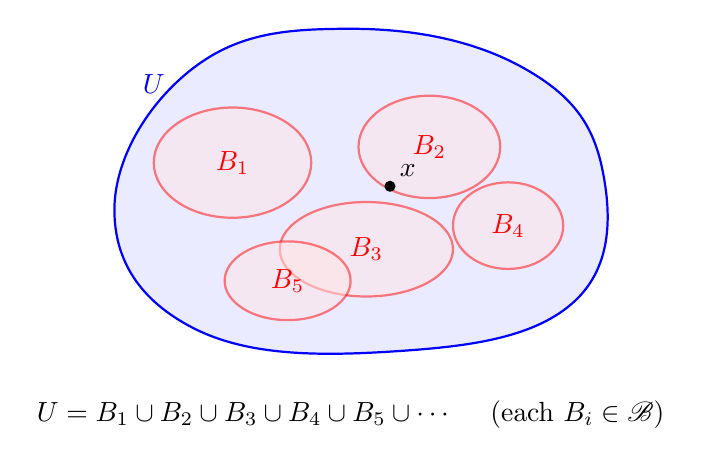
\begin{tikzpicture}[scale=1.0]
    % The ambient open set U
    \draw[thick, blue, fill=blue!8]
        plot[smooth cycle, tension=0.7]
        coordinates {(-3,0) (-2,1.8) (0,2.3) (2.2,1.8) (3.2,0.5)
                     (2.8,-1.2) (0.5,-1.8) (-2,-1.5)};
    \node[blue] at (-2.5,1.6) {$U$};

    % Base elements covering U
    \draw[thick, red, fill=red!10, opacity=0.5]
        (-1.5,0.6) ellipse (1.0 and 0.7);
    \node[red] at (-1.5,0.6) {$B_1$};

    \draw[thick, red, fill=red!10, opacity=0.5]
        (1.0,0.8) ellipse (0.9 and 0.65);
    \node[red] at (1.0,0.8) {$B_2$};

    \draw[thick, red, fill=red!10, opacity=0.5]
        (0.2,-0.5) ellipse (1.1 and 0.6);
    \node[red] at (0.2,-0.5) {$B_3$};

    \draw[thick, red, fill=red!10, opacity=0.5]
        (2.0,-0.2) ellipse (0.7 and 0.55);
    \node[red] at (2.0,-0.2) {$B_4$};

    \draw[thick, red, fill=red!10, opacity=0.5]
        (-0.8,-0.9) ellipse (0.8 and 0.5);
    \node[red] at (-0.8,-0.9) {$B_5$};

    % Point x with its base element
    \fill (0.5,0.3) circle (2pt);
    \node[above right] at (0.5,0.3) {$x$};

    % Caption
    \node[below] at (0,-2.3) {%
        $U = B_1\cup B_2\cup B_3\cup B_4\cup B_5\cup\cdots$
        \quad (each $B_i\in\mathscr{B}$)};
\end{tikzpicture}
\end{center}

%----------------------------------------------------------
\section{Counterexample: the Sorgenfrey line}
\label{sec:sorgenfrey-counterexample}

\begin{proposition}
\label{prop:sorgenfrey-first-countable}
\index{Sorgenfrey line!first countable}
The Sorgenfrey line $\mathbb{R}_\ell$ is first countable.
\end{proposition}

\begin{proof}
For each $x\in\mathbb{R}$, the collection
$\{[x, x+1/n) : n\in\mathbb{N},\;n\ge 1\}$ is a countable neighborhood base
at $x$.  Indeed, if $U$ is open in $\mathbb{R}_\ell$ and $x\in U$, there exist
$a\le x<b$ with $[a,b)\subseteq U$; then for $n$ large enough,
$[x,x+1/n)\subseteq [a,b)\subseteq U$.
\end{proof}

\begin{proposition}
\label{prop:sorgenfrey-separable}
\index{Sorgenfrey line!separable}
The Sorgenfrey line $\mathbb{R}_\ell$ is separable.
\end{proposition}

\begin{proof}
The set $\mathbb{Q}$ is dense in $\mathbb{R}_\ell$: every nonempty basic open
set $[a,b)$ with $a<b$ contains a rational number.
\end{proof}

\begin{proposition}
\label{prop:sorgenfrey-not-second-countable}
\index{Sorgenfrey line!not second countable}
The Sorgenfrey line $\mathbb{R}_\ell$ is not second countable.
\end{proposition}

\begin{proof}
Suppose for contradiction that $\mathscr{B}=\{B_n\}_{n\in\mathbb{N}}$ is a
countable base for $\mathbb{R}_\ell$.  For each $x\in\mathbb{R}$, the set
$[x,x+1)$ is open, so there exists $B_{n_x}\in\mathscr{B}$ with
$x\in B_{n_x}\subseteq [x,x+1)$.  Since $x$ is the infimum of $[x,x+1)$ and
$B_{n_x}\subseteq [x,x+1)$ with $x\in B_{n_x}$, we see that $\inf B_{n_x}=x$.
Therefore the map $x\mapsto n_x$ is injective (distinct reals yield distinct
indices), giving an injection $\mathbb{R}\hookrightarrow\mathbb{N}$, which
contradicts the uncountability of $\mathbb{R}$.
\end{proof}

%----------------------------------------------------------
\section{Worked examples}
\label{sec:bases-worked}

\begin{example}[Comparing bases]
\label{ex:comparing-bases}
\index{base!comparison}
Let $\mathscr{B}_1=\{(a,b):a<b\}$ and
$\mathscr{B}_2=\{[a,b):a<b\}$ be bases on $\mathbb{R}$.  We show
$\mathscr{T}_{\mathscr{B}_2}$ is strictly finer than
$\mathscr{T}_{\mathscr{B}_1}$.

\emph{$\mathscr{T}_{\mathscr{B}_1}\subseteq\mathscr{T}_{\mathscr{B}_2}$:}\;
Given $(a,b)$ and $x\in(a,b)$, we have $[x,b)\subseteq(a,b)$, so each standard
open set is a union of Sorgenfrey-open sets.

\emph{Strict containment:}\; The set $[0,1)$ is open in
$\mathscr{T}_{\mathscr{B}_2}$ but not in $\mathscr{T}_{\mathscr{B}_1}$,
since no open interval $(a,b)$ contains $0$ and is contained in $[0,\infty)$
with $b\le 1$ while also having $a<0$; more precisely, $0$ has no standard
neighborhood contained in $[0,1)$.
\end{example}

\begin{example}[Product topology sub-base]
\label{ex:product-subbase}
\index{sub-base!product topology}
Let $X_1,X_2$ be topological spaces with topologies $\mathscr{T}_1,\mathscr{T}_2$.
The collection
\[
    \mathscr{S}
    = \{\pi_1^{-1}(U_1) : U_1\in\mathscr{T}_1\}
      \cup
      \{\pi_2^{-1}(U_2) : U_2\in\mathscr{T}_2\}
\]
is a sub-base for the product topology on $X_1\times X_2$.  A finite
intersection of sub-base elements has the form
$\pi_1^{-1}(U_1)\cap\pi_2^{-1}(U_2)=U_1\times U_2$, recovering the standard
base of open rectangles.
\end{example}

\begin{example}[A topology from a sub-base on a finite set]
\label{ex:finite-subbase}
Let $X=\{1,2,3\}$ and $\mathscr{S}=\bigl\{\{1,2\},\{2,3\}\bigr\}$.  Then
$\mathscr{S}$ covers $X$ since $\{1,2\}\cup\{2,3\}=X$.  The finite
intersections of members of $\mathscr{S}$ are $\{1,2\}$, $\{2,3\}$, and
$\{1,2\}\cap\{2,3\}=\{2\}$.  Taking all unions, the generated topology is
\[
    \mathscr{T}
    = \bigl\{\varnothing,\;\{2\},\;\{1,2\},\;\{2,3\},\;\{1,2,3\}\bigr\}.
\]
Note that $\{1\}$ and $\{3\}$ are not open.
\end{example}

\begin{example}[Countable base for a metric space]
\label{ex:countable-base-metric}
Let $(X,d)$ be a separable metric space with countable dense subset $D$.  Then
$\mathscr{B}=\{B_d(q,1/n) : q\in D,\;n\in\mathbb{N}_{\ge 1}\}$ is a
countable base, so $(X,d)$ is second countable.  Thus, for metric spaces,
separability and second countability are equivalent.
\end{example}

%----------------------------------------------------------
\section{Exercises}
\label{sec:bases-exercises}

\begin{exercise}[$\star$]
\label{exer:base-discrete}
Show that the collection of singletons $\bigl\{\{x\}:x\in X\bigr\}$ is a base
for the discrete topology on $X$.
\end{exercise}

\begin{exercise}[$\star$]
\label{exer:base-cofinite}
Let $X$ be an infinite set.  Does the cofinite topology on $X$ have a countable
base?  Justify your answer.
\end{exercise}

\begin{exercise}[$\star$]
\label{exer:subbase-finite-complement}
Let $X=\mathbb{R}$ and $\mathscr{S}=\{\mathbb{R}\setminus\{x\}:x\in\mathbb{R}\}$.
Show that $\mathscr{S}$ is a sub-base for the cofinite topology on~$\mathbb{R}$.
\end{exercise}

\begin{exercise}[$\star\star$]
\label{exer:base-comparison-lemma}
Let $\mathscr{B}$ and $\mathscr{B}'$ be bases for topologies $\mathscr{T}$ and
$\mathscr{T}'$ on $X$.  Show that $\mathscr{T}\subseteq\mathscr{T}'$ if and
only if for every $B\in\mathscr{B}$ and $x\in B$ there exists
$B'\in\mathscr{B}'$ with $x\in B'\subseteq B$.
\end{exercise}

\begin{exercise}[$\star\star$]
\label{exer:second-countable-subspace}
Show that every subspace of a second countable space is second countable.
\end{exercise}

\begin{exercise}[$\star\star$]
\label{exer:separable-not-2nd-countable}
Give an example of a topological space that is separable but not second
countable.  (\textit{Hint:} consider the Sorgenfrey line, or an uncountable set
with a suitable topology.)
\end{exercise}

\begin{exercise}[$\star\star$]
\label{exer:lindelof-metrizable}
Let $X$ be a metrizable Lindel\"{o}f space.  Show that $X$ is second countable.
(\textit{Hint:} for each $n$, cover $X$ by balls of radius $1/n$.)
\end{exercise}

\begin{exercise}[$\star\star\star$]
\label{exer:sorgenfrey-product}
Show that the Sorgenfrey plane $\mathbb{R}_\ell\times\mathbb{R}_\ell$ is
separable but not Lindel\"{o}f.  (\textit{Hint:} consider the anti-diagonal
$\{(x,-x):x\in\mathbb{R}\}$ and cover it by basic open sets.)
\end{exercise}

\begin{exercise}[$\star\star\star$]
\label{exer:generated-topology-lattice}
Let $\mathscr{A}$ and $\mathscr{B}$ be collections of subsets of $X$.  Prove
that $\mathscr{T}(\mathscr{A}\cup\mathscr{B})$ is the smallest topology
containing both $\mathscr{T}(\mathscr{A})$ and $\mathscr{T}(\mathscr{B})$.  Is
$\mathscr{T}(\mathscr{A}\cup\mathscr{B})=
\mathscr{T}(\mathscr{A})\cup\mathscr{T}(\mathscr{B})$ in general?  Give a
proof or counterexample.
\end{exercise}

%----------------------------------------------------------
\section*{Chapter summary}
\addcontentsline{toc}{section}{Chapter summary}

\begin{itemize}
    \item A \textbf{base} for a topology is a sub-collection such that every
        open set is a union of base elements.  The base criterion
        (Theorem~\ref{thm:base-criterion}) provides a direct test.
    \item A \textbf{sub-base} generates a topology by first taking all finite
        intersections (to produce a base) and then all unions.
    \item The \textbf{generated topology} $\mathscr{T}(\mathscr{A})$ is the
        intersection of all topologies containing $\mathscr{A}$.
    \item \textbf{Second countable} $\Rightarrow$ \textbf{separable}
        $\Rightarrow$ (in metrizable spaces) second countable.
    \item \textbf{Second countable} $\Rightarrow$ \textbf{Lindel\"{o}f}.
    \item The Sorgenfrey line is first countable and separable, but not second
        countable, demonstrating that the converses fail.
\end{itemize}

\index{base|)}
\index{sub-base|)}

%==========================================================
% CHAPTER 4 — Continuity, Homeomorphisms, and Topological Invariants
%==========================================================
\chapter{Continuity, Homeomorphisms, and Topological Invariants}
\label{ch:continuity}
\index{continuity|(}
\index{homeomorphism|(}

The notion of a continuous function lies at the very heart of topology.  In
real analysis, continuity is defined via the $\varepsilon$-$\delta$ formalism:
$f\colon\mathbb{R}\to\mathbb{R}$ is continuous at $x_0$ if for every
$\varepsilon>0$ there exists $\delta>0$ such that $|x-x_0|<\delta$ implies
$|f(x)-f(x_0)|<\varepsilon$.  A standard exercise shows that this is
equivalent to requiring that the preimage of every open set be open.  It is
precisely this preimage formulation that generalizes to arbitrary topological
spaces, freeing the concept of continuity from any dependence on a metric.  We
then single out the most important class of continuous maps---the
\emph{homeomorphisms}---and introduce the fundamental idea of a topological
invariant.

%----------------------------------------------------------
\section{Continuous maps}
\label{sec:continuous-maps}

\begin{definition}[Continuous map]
\label{def:continuous}
\index{continuity!definition}
Let $(X,\mathscr{T}_X)$ and $(Y,\mathscr{T}_Y)$ be topological spaces.  A
function $f\colon X\to Y$ is \textbf{continuous} if for every open set
$V\in\mathscr{T}_Y$, the preimage $f^{-1}(V)$ belongs to $\mathscr{T}_X$.
\end{definition}

\begin{theorem}[Equivalent characterizations of continuity]
\label{thm:continuity-equiv}
\index{continuity!equivalent characterizations}
Let $f\colon X\to Y$ be a function between topological spaces.  The following
are equivalent:
\begin{enumerate}
    \item \label{item:cont-open}
        $f$ is continuous (preimages of open sets are open).
    \item \label{item:cont-closed}
        For every closed set $C\subseteq Y$, the preimage $f^{-1}(C)$ is
        closed in $X$.
    \item \label{item:cont-closure}
        For every subset $A\subseteq X$,\;
        $f\bigl(\overline{A}\bigr)\subseteq\overline{f(A)}$.
    \item \label{item:cont-interior}
        For every subset $B\subseteq Y$,\;
        $f^{-1}\bigl(\operatorname{Int}(B)\bigr)\subseteq
        \operatorname{Int}\bigl(f^{-1}(B)\bigr)$.
    \item \label{item:cont-nbhd}
        For every $x\in X$ and every neighborhood $V$ of $f(x)$ in $Y$, the
        preimage $f^{-1}(V)$ is a neighborhood of $x$ in $X$.
\end{enumerate}
\end{theorem}

\begin{proof}
\textbf{(\ref{item:cont-open})$\Leftrightarrow$(\ref{item:cont-closed}):}\;
A set $C$ is closed in $Y$ if and only if $Y\setminus C$ is open.  Since
$f^{-1}(Y\setminus C)=X\setminus f^{-1}(C)$, we see that $f^{-1}(C)$ is
closed in $X$ if and only if $f^{-1}(Y\setminus C)$ is open in $X$.  Hence the
equivalence.

\medskip\noindent
\textbf{(\ref{item:cont-closed})$\Rightarrow$(\ref{item:cont-closure}):}\;
Let $A\subseteq X$.  The set $\overline{f(A)}$ is closed in $Y$, so by
(\ref{item:cont-closed}), $f^{-1}\bigl(\overline{f(A)}\bigr)$ is closed in
$X$.  Since $A\subseteq f^{-1}(f(A))\subseteq
f^{-1}\bigl(\overline{f(A)}\bigr)$ and the latter is closed,
$\overline{A}\subseteq f^{-1}\bigl(\overline{f(A)}\bigr)$.  Applying $f$,
$f(\overline{A})\subseteq\overline{f(A)}$.

\medskip\noindent
\textbf{(\ref{item:cont-closure})$\Rightarrow$(\ref{item:cont-closed}):}\;
Let $C\subseteq Y$ be closed.  Set $A=f^{-1}(C)$.  By~(\ref{item:cont-closure}),
$f(\overline{A})\subseteq\overline{f(A)}\subseteq\overline{C}=C$.  Hence
$\overline{A}\subseteq f^{-1}(C)=A$, so $A$ is closed.

\medskip\noindent
\textbf{(\ref{item:cont-open})$\Rightarrow$(\ref{item:cont-interior}):}\;
Let $B\subseteq Y$.  Since $\operatorname{Int}(B)$ is open in $Y$,
$f^{-1}(\operatorname{Int}(B))$ is open in $X$ by~(\ref{item:cont-open}).
Moreover, $f^{-1}(\operatorname{Int}(B))\subseteq f^{-1}(B)$.  Since
$f^{-1}(\operatorname{Int}(B))$ is an open subset of $f^{-1}(B)$, it is
contained in $\operatorname{Int}(f^{-1}(B))$.

\medskip\noindent
\textbf{(\ref{item:cont-interior})$\Rightarrow$(\ref{item:cont-open}):}\;
Let $V$ be open in $Y$.  Then $\operatorname{Int}(V)=V$, so
$f^{-1}(V)=f^{-1}(\operatorname{Int}(V))\subseteq
\operatorname{Int}(f^{-1}(V))\subseteq f^{-1}(V)$.  Equality holds throughout,
so $f^{-1}(V)=\operatorname{Int}(f^{-1}(V))$, meaning $f^{-1}(V)$ is open.

\medskip\noindent
\textbf{(\ref{item:cont-open})$\Leftrightarrow$(\ref{item:cont-nbhd}):}\;
If $f$ is continuous and $V$ is a neighborhood of $f(x)$, there exists an open
set $U$ with $f(x)\in U\subseteq V$.  Then $x\in f^{-1}(U)\subseteq f^{-1}(V)$
and $f^{-1}(U)$ is open, so $f^{-1}(V)$ is a neighborhood of $x$.  Conversely,
if (\ref{item:cont-nbhd}) holds and $V$ is open in $Y$, then for every
$x\in f^{-1}(V)$, $V$ is a neighborhood of $f(x)$, so $f^{-1}(V)$ is a
neighborhood of $x$; hence $f^{-1}(V)$ is a neighborhood of each of its points,
so it is open.
\end{proof}

\begin{theorem}[Composition of continuous maps]
\label{thm:composition-continuous}
\index{continuity!composition}
If $f\colon X\to Y$ and $g\colon Y\to Z$ are continuous, then
$g\circ f\colon X\to Z$ is continuous.
\end{theorem}

\begin{proof}
Let $W$ be open in $Z$.  Since $g$ is continuous, $g^{-1}(W)$ is open in $Y$.
Since $f$ is continuous, $f^{-1}(g^{-1}(W))$ is open in $X$.  But
$(g\circ f)^{-1}(W)=f^{-1}(g^{-1}(W))$, so $(g\circ f)^{-1}(W)$ is open
in~$X$.
\end{proof}

%----------------------------------------------------------
\section{Homeomorphisms and topological invariants}
\label{sec:homeomorphisms}

\begin{definition}[Homeomorphism]
\label{def:homeomorphism}
\index{homeomorphism!definition}
A function $f\colon X\to Y$ is a \textbf{homeomorphism} if $f$ is a bijection
and both $f$ and $f^{-1}$ are continuous.  When such a map exists, $X$ and $Y$
are said to be \textbf{homeomorphic}, written $X\cong Y$.
\end{definition}

\begin{definition}[Topological property / invariant]
\label{def:topological-invariant}
\index{topological invariant}
A property of a topological space is a \textbf{topological invariant} (or
\textbf{topological property}) if it is preserved by homeomorphisms; that is,
if $X$ has the property and $X\cong Y$, then $Y$ has the property as well.
\end{definition}

\begin{remark}
\label{rem:invariant-examples}
Examples of topological invariants include: being Hausdorff, being compact,
being connected, being second countable, cardinality of the space, and
the fundamental group $\pi_1(X,x_0)$.
\end{remark}

%----------------------------------------------------------
\section{Open, closed, and continuous maps}
\label{sec:open-closed-maps}

\begin{definition}[Open and closed maps]
\label{def:open-closed-maps}
\index{open map}
\index{closed map}
A function $f\colon X\to Y$ is called
\begin{itemize}
    \item an \textbf{open map} if for every open set $U\subseteq X$, the image
        $f(U)$ is open in $Y$;
    \item a \textbf{closed map} if for every closed set $C\subseteq X$, the
        image $f(C)$ is closed in $Y$.
\end{itemize}
\end{definition}

\begin{remark}
\label{rem:open-closed-continuous}
These notions are logically independent of continuity.  A continuous map need
not be open or closed, and an open (or closed) map need not be continuous.
\end{remark}

\begin{example}[Continuous but not open]
\label{ex:cont-not-open}
The constant function $f\colon\mathbb{R}\to\mathbb{R}$, $f(x)=0$, is
continuous.  However, $f(\mathbb{R})=\{0\}$, which is not open in
$\mathbb{R}$.  So $f$ is continuous but not an open map.
\end{example}

\begin{example}[Open but not continuous]
\label{ex:open-not-cont}
\index{open map!not continuous}
Let $X=\mathbb{R}$ with the discrete topology and $Y=\mathbb{R}$ with the
standard topology.  Consider $f\colon Y\to X$ defined by $f(x)=x$.  Every
subset of $X$ is open, so the image of any set under $f$ is open in $X$;
hence $f\colon Y\to X$ is an open map.  But $f$ is not continuous: the
singleton $\{0\}$ is open in $X$ (discrete topology) while $f^{-1}(\{0\})=\{0\}$
is not open in $Y$ (standard topology).
\end{example}

\begin{example}[Closed but not continuous]
\label{ex:closed-not-cont}
\index{closed map!not continuous}
Let $X=\mathbb{R}$ with the standard topology and $Y=\mathbb{R}$ with the
indiscrete topology.  The identity $f\colon X\to Y$, $f(x)=x$, maps every
set to itself.  In $Y$ the only closed sets are $\varnothing$ and
$\mathbb{R}$, so $f$ is vacuously closed (the only closed images we need to
check collapse to $\varnothing$ or $\mathbb{R}$).  But $f$ is not
continuous: $Y\setminus\varnothing = \mathbb{R}$ is the only nonempty open
set in $Y$, yet many open sets in $Y$ (there are only two) pull back to open
sets in~$X$; more precisely, $f^{-1}$ from the indiscrete topology gives
only $\varnothing$ and $\mathbb{R}$ as open, but in $X$ open sets like
$(0,1)$ have $f^{-1}((0,1))=(0,1)$ --- wait, $f$ goes $X\to Y$, and
$(0,1)$ is not open in $Y$.  So $f$ is trivially continuous.  To correct:
let $g\colon Y\to X$ (from indiscrete to standard).  Then $g$ is closed
because the closed sets in $Y$ are $\varnothing$ and $\mathbb{R}$, and
$g(\varnothing)=\varnothing$, $g(\mathbb{R})=\mathbb{R}$, both closed in
$X$.  But $g$ is not continuous: $(0,1)$ is open in $X$ while
$g^{-1}((0,1))=(0,1)$ is not open in the indiscrete topology on~$Y$.
\end{example}

\begin{proposition}
\label{prop:homeo-iff-cont-open-bij}
\index{homeomorphism!characterization}
A function $f\colon X\to Y$ is a homeomorphism if and only if $f$ is a
continuous open bijection; equivalently, if and only if $f$ is a continuous
closed bijection.
\end{proposition}

\begin{proof}
If $f$ is a homeomorphism, then $f$ is a continuous bijection and $f^{-1}$ is
continuous.  For any open $U\subseteq X$,
$f(U)=(f^{-1})^{-1}(U)$ is open in $Y$ since $f^{-1}$ is continuous; so $f$
is open.  Conversely, if $f$ is a continuous open bijection, then for any open
$U\subseteq X$, $(f^{-1})^{-1}(U)=f(U)$ is open, so $f^{-1}$ is continuous.
The argument for ``closed'' is analogous, replacing ``open'' by ``closed''
throughout.
\end{proof}

%----------------------------------------------------------
\section{A compact-to-Hausdorff theorem}
\label{sec:compact-hausdorff}

\begin{theorem}
\label{thm:cont-bij-compact-hausdorff}
\index{homeomorphism!compact to Hausdorff}
\index{compact!continuous bijection to Hausdorff}
Let $f\colon X\to Y$ be a continuous bijection.  If $X$ is compact and $Y$ is
Hausdorff, then $f$ is a homeomorphism.
\end{theorem}

\begin{proof}
By Proposition~\ref{prop:homeo-iff-cont-open-bij}, it suffices to show that
$f$ is a closed map.  Let $C\subseteq X$ be closed.  Since $X$ is compact
and $C$ is a closed subset of a compact space, $C$ is compact.  The continuous
image of a compact set is compact, so $f(C)$ is compact in $Y$.  Since $Y$ is
Hausdorff, every compact subset of $Y$ is closed.  Therefore $f(C)$ is closed
in $Y$.  Hence $f$ is a closed map, and since it is also a continuous
bijection, it is a homeomorphism.
\end{proof}

%----------------------------------------------------------
\section{Topological embeddings}
\label{sec:embeddings}

\begin{definition}[Topological embedding]
\label{def:embedding}
\index{embedding!topological}
A function $f\colon X\to Y$ is a \textbf{topological embedding} (or simply an
\textbf{embedding}) if $f$ is an injective continuous map such that
$f\colon X\to f(X)$ is a homeomorphism, where $f(X)$ carries the subspace
topology inherited from $Y$.
\end{definition}

\begin{remark}
\label{rem:embedding-equiv}
Equivalently, $f\colon X\to Y$ is an embedding if and only if $f$ is injective,
continuous, and for every open $U\subseteq X$ there exists an open
$V\subseteq Y$ with $f(U)=V\cap f(X)$.
\end{remark}

\begin{example}
\label{ex:embedding-interval}
The inclusion $\iota\colon (0,1)\hookrightarrow\mathbb{R}$, $\iota(x)=x$, is
a topological embedding.  More generally, the inclusion of any subspace into
the ambient space is always an embedding.
\end{example}

%----------------------------------------------------------
\section{The pasting lemma}
\label{sec:pasting-lemma}

\begin{theorem}[Pasting lemma]
\label{thm:pasting-lemma}
\index{pasting lemma}
Let $X=A\cup B$ where $A$ and $B$ are closed subsets of $X$.  Let
$f\colon A\to Y$ and $g\colon B\to Y$ be continuous functions that agree on
the overlap: $f(x)=g(x)$ for all $x\in A\cap B$.  Then the function
$h\colon X\to Y$ defined by
\[
    h(x)=
    \begin{cases}
        f(x) & \text{if } x\in A,\\
        g(x) & \text{if } x\in B,
    \end{cases}
\]
is continuous.
\end{theorem}

\begin{proof}
We use the characterization of continuity via closed sets
(Theorem~\ref{thm:continuity-equiv}, (\ref{item:cont-closed})).  Let
$C\subseteq Y$ be closed.  Then
\[
    h^{-1}(C)
    = \{x\in X : h(x)\in C\}
    = \{x\in A : f(x)\in C\}\cup\{x\in B : g(x)\in C\}
    = f^{-1}(C)\cup g^{-1}(C).
\]
Since $f\colon A\to Y$ is continuous and $C$ is closed in $Y$, the set
$f^{-1}(C)$ is closed in the subspace $A$.  Because $A$ is closed in $X$, a
set closed in $A$ is closed in $X$ (a closed subset of a closed set is
closed).  Hence $f^{-1}(C)$ is closed in $X$.  By the same reasoning,
$g^{-1}(C)$ is closed in $X$.  A finite union of closed sets is closed, so
$h^{-1}(C)=f^{-1}(C)\cup g^{-1}(C)$ is closed in $X$.  Therefore $h$ is
continuous.
\end{proof}

\begin{remark}
\label{rem:pasting-open}
An analogous statement holds when $A$ and $B$ are both \emph{open} (and the
proof is even simpler, working directly with open sets).  The lemma generalizes
to finite covers by closed sets $X=A_1\cup\cdots\cup A_n$, but \emph{not} to
arbitrary covers by closed sets.
\end{remark}

%----------------------------------------------------------
\section{Key examples and constructions}
\label{sec:continuity-examples}

\begin{example}[$(0,1)\cong\mathbb{R}$]
\label{ex:01-homeo-R}
\index{homeomorphism!$(0,1)\cong\mathbb{R}$}
Define $f\colon(0,1)\to\mathbb{R}$ by
\[
    f(x) = \tan\!\Bigl(\pi\Bigl(x-\tfrac{1}{2}\Bigr)\Bigr).
\]
This is a composition of continuous functions: $x\mapsto \pi(x-\frac{1}{2})$
(affine, hence continuous) followed by $\tan$ (continuous on
$(-\pi/2,\pi/2)$).  The map $f$ is a bijection from $(0,1)$ onto $\mathbb{R}$
with continuous inverse $f^{-1}(y)=\frac{1}{\pi}\arctan(y)+\frac{1}{2}$.
Therefore $f$ is a homeomorphism.  In particular, $(0,1)$ and $\mathbb{R}$ are
homeomorphic.
\end{example}

\begin{example}[Stereographic projection]
\label{ex:stereographic}
\index{stereographic projection}
Let $S^n=\{\mathbf{x}\in\mathbb{R}^{n+1}:|\mathbf{x}|=1\}$ denote the
$n$-sphere and let $N=(0,\ldots,0,1)$ be its north pole.  The stereographic
projection $\sigma\colon S^n\setminus\{N\}\to\mathbb{R}^n$ is defined by
\[
    \sigma(x_1,\ldots,x_{n+1})
    = \frac{1}{1-x_{n+1}}(x_1,\ldots,x_n).
\]
One verifies that $\sigma$ is a bijection with inverse
\[
    \sigma^{-1}(u_1,\ldots,u_n)
    = \frac{1}{|\mathbf{u}|^2+1}
      \bigl(2u_1,\ldots,2u_n,\,|\mathbf{u}|^2-1\bigr),
\]
and both maps are continuous (being compositions of rational functions with
nonvanishing denominators).  Hence $S^n\setminus\{N\}\cong\mathbb{R}^n$.
\end{example}

%----------------------------------------------------------
\section{Visualizations}
\label{sec:continuity-tikz}

\paragraph{Homeomorphism between $(0,1)$ and $\mathbb{R}$.}

\begin{center}
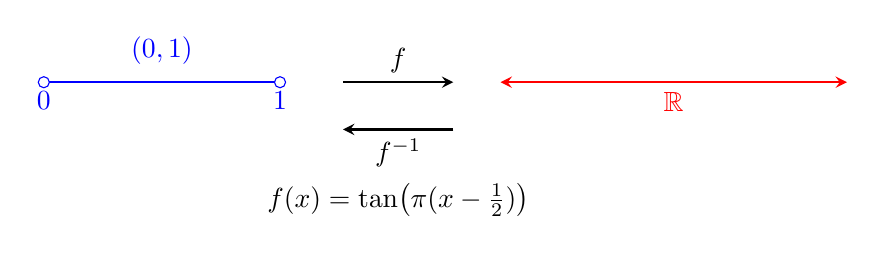
\begin{tikzpicture}[scale=1.0, >=stealth]
    % Domain (0,1)
    \draw[thick, blue] (0,0) -- (3,0);
    \draw[blue, fill=white] (0,0) circle (2pt);
    \draw[blue, fill=white] (3,0) circle (2pt);
    \node[below, blue] at (0,0) {$0$};
    \node[below, blue] at (3,0) {$1$};
    \node[above, blue] at (1.5,0.1) {$(0,1)$};

    % Arrow
    \draw[->, thick] (3.8,0) -- (5.2,0);
    \node[above] at (4.5,0) {$f$};

    % Codomain R
    \draw[thick, red, <->] (5.8,0) -- (10.2,0);
    \node[below, red] at (8,0) {$\mathbb{R}$};

    % Inverse arrow
    \draw[->, thick] (5.2,-0.6) -- (3.8,-0.6);
    \node[below] at (4.5,-0.6) {$f^{-1}$};

    % Function label
    \node at (4.5,-1.5) {$f(x)=\tan\bigl(\pi(x-\tfrac{1}{2})\bigr)$};
\end{tikzpicture}
\end{center}

\paragraph{Open, closed, and continuous maps.}

\begin{center}
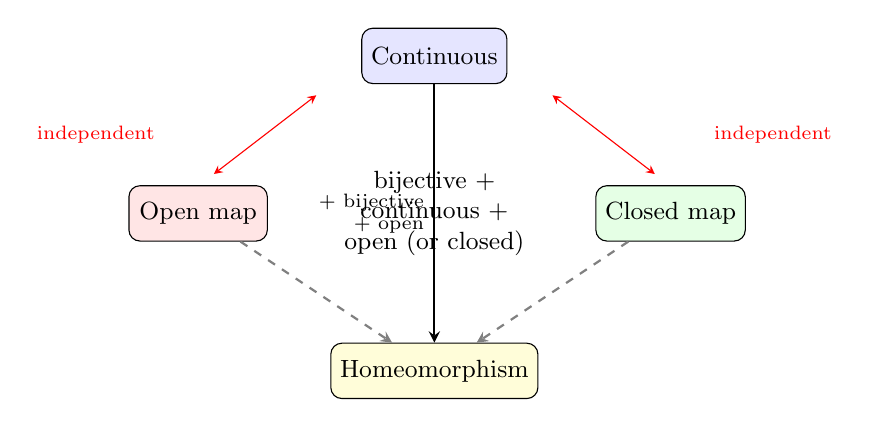
\begin{tikzpicture}[
    >=stealth,
    block/.style={rectangle, draw, rounded corners, minimum height=2em,
                  minimum width=5em, text centered, font=\small},
    arr/.style={->, thick}
]
    \node[block, fill=blue!10] (cont)  at (0,0)   {Continuous};
    \node[block, fill=red!10]  (open)  at (-3,-2)  {Open map};
    \node[block, fill=green!10](closed) at (3,-2)  {Closed map};
    \node[block, fill=yellow!15](homeo) at (0,-4)  {Homeomorphism};

    \node[font=\small, text width=3cm, align=center] at (0,-2)
        {bijective $+$\\continuous $+$\\open (or closed)};

    \draw[arr] (cont)  -- node[left, font=\scriptsize, text width=2cm, align=right]
        {$+$ bijective\\$+$ open} (homeo);
    \draw[arr, dashed, gray] (open)  -- (homeo);
    \draw[arr, dashed, gray] (closed) -- (homeo);

    % Independence labels
    \node[font=\scriptsize, red] at (-4.3,-1) {independent};
    \draw[<->, red, thin] (-1.5,-0.5) -- (-2.8,-1.5);
    \node[font=\scriptsize, red] at (4.3,-1) {independent};
    \draw[<->, red, thin] (1.5,-0.5) -- (2.8,-1.5);
\end{tikzpicture}
\end{center}

%----------------------------------------------------------
\section{Counterexample: a continuous bijection that is not a homeomorphism}
\label{sec:counterexample-circle}

\begin{example}
\label{ex:cont-bij-not-homeo}
\index{homeomorphism!continuous bijection that is not}
Define $f\colon[0,2\pi)\to S^1$ by $f(t)=(\cos t,\sin t)$, where $[0,2\pi)$
carries the subspace topology from $\mathbb{R}$ and $S^1$ carries the subspace
topology from $\mathbb{R}^2$.  Then $f$ is a continuous bijection.

However, $f$ is \emph{not} a homeomorphism.  To see this, consider the set
$U=[0,1)$, which is open in $[0,2\pi)$ (as $[0,1)=[0,2\pi)\cap(-1,1)$).
Its image $f(U)$ is the arc $\{(\cos t,\sin t):0\le t<1\}$.  This arc
contains the point $(1,0)=f(0)$, but every open neighborhood of $(1,0)$ in
$S^1$ contains points $(\cos t,\sin t)$ with $t$ slightly less than $2\pi$,
which lie outside $f(U)$.  Hence $f(U)$ is not open in $S^1$, so $f$ is not
an open map, and therefore $f^{-1}$ is not continuous.

Note that $[0,2\pi)$ is not compact (it is not closed in $\mathbb{R}$, and
in particular it is not a closed bounded subset of $\mathbb{R}$), so
Theorem~\ref{thm:cont-bij-compact-hausdorff} does not apply.
\end{example}

%----------------------------------------------------------
\section{Invariance of domain}
\label{sec:invariance-domain}

\begin{theorem}[Invariance of domain --- Brouwer, 1912]
\label{thm:invariance-domain}
\index{invariance of domain}
Let $U\subseteq\mathbb{R}^n$ be open and let $f\colon U\to\mathbb{R}^n$ be a
continuous injective map.  Then $f(U)$ is open in $\mathbb{R}^n$, and
$f\colon U\to f(U)$ is a homeomorphism.
\end{theorem}

\begin{remark}
\label{rem:invariance-domain-significance}
The proof of invariance of domain requires tools from algebraic topology
(specifically, homology theory) and is beyond the scope of this course.
Nevertheless, the result has profound consequences:
\begin{enumerate}
    \item It implies that $\mathbb{R}^m\cong\mathbb{R}^n$ only if $m=n$,
        establishing that \emph{topological dimension} is a well-defined
        invariant of Euclidean spaces.
    \item It guarantees that any continuous injection from an open subset of
        $\mathbb{R}^n$ into $\mathbb{R}^n$ is automatically an open map (and
        hence an embedding), a fact that fails in general topological spaces.
    \item It shows that the notion of ``dimension'' in $\mathbb{R}^n$ is a
        topological invariant, not merely an algebraic artifact.
\end{enumerate}
\end{remark}

%----------------------------------------------------------
\section{Worked examples}
\label{sec:continuity-worked}

\begin{example}[Continuity via sub-base]
\label{ex:continuity-subbase}
\index{continuity!via sub-base}
Let $f\colon X\to Y$ be a function and let $\mathscr{S}$ be a sub-base for the
topology on $Y$.  Then $f$ is continuous if and only if $f^{-1}(S)$ is open in
$X$ for every $S\in\mathscr{S}$.

\emph{Proof.}\; The ``only if'' direction is immediate.  For the converse,
suppose $f^{-1}(S)$ is open for all $S\in\mathscr{S}$.  Every basic open set
is a finite intersection $S_1\cap\cdots\cap S_n$, and
$f^{-1}(S_1\cap\cdots\cap S_n)=f^{-1}(S_1)\cap\cdots\cap f^{-1}(S_n)$, a
finite intersection of open sets, hence open.  Every open set is a union of
basic open sets, and $f^{-1}$ commutes with unions, so the preimage of every
open set is open.
\end{example}

\begin{example}[The projection map is continuous and open but not closed]
\label{ex:projection}
\index{projection!continuous and open}
Let $\pi_1\colon\mathbb{R}^2\to\mathbb{R}$ be the projection
$\pi_1(x,y)=x$.  The preimage of an open set $(a,b)\subseteq\mathbb{R}$ is
$(a,b)\times\mathbb{R}$, which is open in $\mathbb{R}^2$, so $\pi_1$ is
continuous.  For any basic open set $U\times V\subseteq\mathbb{R}^2$ (with $U,V$
open in $\mathbb{R}$), $\pi_1(U\times V)=U$ (provided $V\neq\varnothing$),
which is open; hence $\pi_1$ is an open map.  However, $\pi_1$ is not closed:
the set $C=\{(x,y):xy=1\}$ is closed in $\mathbb{R}^2$ (it is the preimage
of $\{1\}$ under the continuous map $(x,y)\mapsto xy$), but
$\pi_1(C)=\mathbb{R}\setminus\{0\}$, which is not closed in $\mathbb{R}$.
\end{example}

\begin{example}[Homeomorphism via the compact-Hausdorff theorem]
\label{ex:compact-hausdorff-app}
Consider the map $f\colon[0,1]/(0\sim 1)\to S^1$ induced by
$t\mapsto(\cos 2\pi t,\sin 2\pi t)$.  The quotient space $[0,1]/(0\sim 1)$
is compact (it is a quotient of a compact space) and $S^1$ is Hausdorff
(as a subspace of $\mathbb{R}^2$).  The map $f$ is a continuous bijection (it
descends from the continuous surjection $t\mapsto(\cos 2\pi t,\sin 2\pi t)$
and becomes injective after the identification $0\sim 1$).  By
Theorem~\ref{thm:cont-bij-compact-hausdorff}, $f$ is a homeomorphism:
$[0,1]/(0\sim 1)\cong S^1$.
\end{example}

%----------------------------------------------------------
\section{Exercises}
\label{sec:continuity-exercises}

\begin{exercise}[$\star$]
\label{exer:const-continuous}
\index{continuity!constant map}
Prove that every constant function $f\colon X\to Y$ is continuous.
\end{exercise}

\begin{exercise}[$\star$]
\label{exer:identity-continuous}
Let $\mathscr{T}_1\subseteq\mathscr{T}_2$ be two topologies on a set $X$.
Show that the identity map $\operatorname{id}\colon(X,\mathscr{T}_2)\to
(X,\mathscr{T}_1)$ is continuous but that the reverse identity
$\operatorname{id}\colon(X,\mathscr{T}_1)\to(X,\mathscr{T}_2)$ need not be.
\end{exercise}

\begin{exercise}[$\star$]
\label{exer:restrict-continuous}
\index{continuity!restriction}
Prove that if $f\colon X\to Y$ is continuous and $A\subseteq X$ carries the
subspace topology, then $f|_A\colon A\to Y$ is continuous.
\end{exercise}

\begin{exercise}[$\star\star$]
\label{exer:closed-graph}
\index{closed graph}
Let $f\colon X\to Y$ be continuous with $Y$ Hausdorff.  Show that the graph
$\Gamma_f=\{(x,f(x)):x\in X\}$ is a closed subset of $X\times Y$.
\end{exercise}

\begin{exercise}[$\star\star$]
\label{exer:homeo-open-intervals}
Prove that any two nonempty open intervals in $\mathbb{R}$ are homeomorphic.
(\textit{Hint:} use affine maps.)
\end{exercise}

\begin{exercise}[$\star\star$]
\label{exer:pasting-three}
State and prove the pasting lemma for three closed sets: if
$X=A\cup B\cup C$ with $A,B,C$ closed, and $f\colon A\to Y$,
$g\colon B\to Y$, $h\colon C\to Y$ are continuous and agree on overlaps, then
the combined function is continuous.
\end{exercise}

\begin{exercise}[$\star\star$]
\label{exer:topological-property}
Show that ``having a countable dense subset'' (separability) is a topological
invariant.
\end{exercise}

\begin{exercise}[$\star\star\star$]
\label{exer:cont-bij-R-to-R2}
\index{space-filling curve}
Show that there is no continuous bijection from $\mathbb{R}$ to
$\mathbb{R}^2$.  (\textit{Hint:} consider removing a point from each and
examine connectedness.)
\end{exercise}

\begin{exercise}[$\star\star\star$]
\label{exer:embedding-characterization}
Let $f\colon X\to Y$ be injective and continuous.  Prove that $f$ is an
embedding if and only if for every open set $U\subseteq X$ and every
$x\in U$, there exists an open set $V\subseteq Y$ such that
$f(x)\in V$ and $f^{-1}(V)\subseteq U$.
\end{exercise}

%----------------------------------------------------------
\section*{Chapter summary}
\addcontentsline{toc}{section}{Chapter summary}

\begin{itemize}
    \item A map $f\colon X\to Y$ is \textbf{continuous} if preimages of open
        sets are open.  Equivalent formulations involve closed sets, closures,
        interiors, or neighborhoods (Theorem~\ref{thm:continuity-equiv}).
    \item The composition of continuous maps is continuous
        (Theorem~\ref{thm:composition-continuous}).
    \item A \textbf{homeomorphism} is a continuous bijection with continuous
        inverse.  Properties preserved under homeomorphisms are
        \textbf{topological invariants}.
    \item Open maps, closed maps, and continuous maps are logically independent
        notions.  A homeomorphism is precisely a continuous open (or closed)
        bijection.
    \item A continuous bijection from a \textbf{compact} space to a
        \textbf{Hausdorff} space is automatically a homeomorphism
        (Theorem~\ref{thm:cont-bij-compact-hausdorff}).
    \item The \textbf{pasting lemma} (Theorem~\ref{thm:pasting-lemma}) allows
        one to build continuous maps from compatible pieces defined on closed
        (or open) subsets.
    \item \textbf{Invariance of domain} guarantees that continuous injections
        from open subsets of $\mathbb{R}^n$ into $\mathbb{R}^n$ are open maps.
\end{itemize}

\index{continuity|)}
\index{homeomorphism|)}
%%%%%%%%%%%%%%%%%%%%%%%%%%%%%%%%%%%%%%%%%%%%%%%%%%%%%%%%%%%%
%  PART 3 — Chapters 5 & 6
%  General Topology: Separation Axioms and Compactness
%%%%%%%%%%%%%%%%%%%%%%%%%%%%%%%%%%%%%%%%%%%%%%%%%%%%%%%%%%%%

%=============================================================
% CHAPTER 5: SEPARATION AXIOMS
%=============================================================
\chapter{Separation Axioms}\label{ch:separation-axioms}
\index{separation axioms|(}

In a metric space $(X,d)$, distinct points $x \neq y$ can always be separated
by disjoint open balls: take $r = d(x,y)/2$ and observe that
$B(x,r) \cap B(y,r) = \varnothing$.  Closed sets can likewise be separated
from points outside them, and even pairs of disjoint closed sets can be
enclosed in disjoint open neighbourhoods.  These properties, however, need not
hold in an arbitrary topological space.  The \emph{separation axioms} form a
hierarchy of increasingly restrictive conditions that a topology may or may not
satisfy, each capturing a different degree of ``separating power.''  This
chapter develops the axioms $T_0$ through $T_4$, proves the strict chain of
implications among them, and illustrates each level with examples and
counterexamples.

%-------------------------------------------------------------
\section{The \texorpdfstring{$T_0$}{T0} Axiom (Kolmogorov Spaces)}
\label{sec:T0}
\index{T0 space@$T_0$ space}\index{Kolmogorov space|see{$T_0$ space}}

\begin{definition}[$T_0$ space]\label{def:T0}
A topological space $(X,\tau)$ is \textbf{$T_0$} (or a \textbf{Kolmogorov
space}\index{Kolmogorov space}) if for every pair of distinct points
$x, y \in X$, there exists an open set $U \in \tau$ that contains exactly one
of them: either $x \in U,\; y \notin U$ or $y \in U,\; x \notin U$.
\end{definition}

\begin{example}[The Sierpi\'nski space]\label{ex:sierpinski-T0}
\index{Sierpinski space@Sierpi\'nski space}
Let $X = \{0,1\}$ with topology $\tau = \{\varnothing, \{1\}, \{0,1\}\}$.
For the pair $0,1$ the open set $\{1\}$ contains $1$ but not~$0$.
Hence $(X,\tau)$ is $T_0$.  Note, however, that no open set contains $0$
without also containing~$1$, so the space is \emph{not} $T_1$.
\end{example}

\begin{example}[Indiscrete space is not $T_0$]\label{ex:indiscrete-not-T0}
\index{indiscrete topology}
If $|X| \ge 2$ and $\tau = \{\varnothing, X\}$, then the only non-empty open
set is $X$ itself, which contains every point.  No pair of distinct points can
be topologically distinguished; thus $(X,\tau)$ is \emph{not} $T_0$.
\end{example}

%-------------------------------------------------------------
\section{The \texorpdfstring{$T_1$}{T1} Axiom}
\label{sec:T1}
\index{T1 space@$T_1$ space}

\begin{definition}[$T_1$ space]\label{def:T1}
A topological space $(X,\tau)$ is \textbf{$T_1$} if for every pair of distinct
points $x, y \in X$, there exists an open set $U$ with $x \in U$ and
$y \notin U$.
\end{definition}

The key difference from $T_0$ is that the requirement is \emph{symmetric}: for
each ordered pair $(x,y)$ with $x \neq y$, a separating open set for $x$ must
exist.

\begin{theorem}[Characterisation of $T_1$ spaces]\label{thm:T1-singletons}
\index{T1 space@$T_1$ space!characterisation}
A topological space $(X,\tau)$ is $T_1$ if and only if every singleton
$\{x\}$ is closed.
\end{theorem}

\begin{proof}
$(\Rightarrow)$ Assume $(X,\tau)$ is $T_1$ and fix $x \in X$.  For every
$y \neq x$ there is an open set $U_y$ with $y \in U_y$ and $x \notin U_y$.
Then
\[
  X \setminus \{x\} = \bigcup_{y \neq x} U_y,
\]
which is a union of open sets and hence open.  Therefore $\{x\}$ is closed.

$(\Leftarrow)$ Suppose every singleton is closed.  Given distinct $x,y$, the
set $U = X \setminus \{y\}$ is open, contains $x$, and does not contain $y$.
Hence $(X,\tau)$ is $T_1$.
\end{proof}

\begin{example}[Cofinite topology]\label{ex:cofinite-T1}
\index{cofinite topology}
Let $X$ be any infinite set and let $\tau_{\mathrm{cof}}$ consist of
$\varnothing$ together with all subsets whose complement is finite.  Every
singleton $\{x\}$ has complement $X \setminus \{x\}$, which is cofinite and
hence open.  By Theorem~\ref{thm:T1-singletons}, $(X,\tau_{\mathrm{cof}})$ is
$T_1$.  We shall see shortly that it is \emph{not} $T_2$.
\end{example}

%-------------------------------------------------------------
\section{The \texorpdfstring{$T_2$}{T2} Axiom (Hausdorff Spaces)}
\label{sec:T2}
\index{T2 space@$T_2$ space}\index{Hausdorff space|see{$T_2$ space}}

\begin{definition}[Hausdorff space]\label{def:T2}
A topological space $(X,\tau)$ is \textbf{$T_2$} (or \textbf{Hausdorff}) if
for every pair of distinct points $x, y \in X$, there exist open sets $U, V$
with $x \in U$, $y \in V$, and $U \cap V = \varnothing$.
\end{definition}

\begin{theorem}[Uniqueness of limits in Hausdorff spaces]
\label{thm:hausdorff-unique-limits}
\index{Hausdorff space!uniqueness of limits}
In a Hausdorff space, a net can converge to at most one point.
\end{theorem}

\begin{proof}
Let $(x_\alpha)_{\alpha \in A}$ be a net in a Hausdorff space $X$ and suppose
$x_\alpha \to x$ and $x_\alpha \to y$ with $x \neq y$.  Choose disjoint open
sets $U \ni x$ and $V \ni y$.  By convergence to $x$, there exists
$\alpha_0$ such that $x_\alpha \in U$ for all $\alpha \ge \alpha_0$.  By
convergence to $y$, there exists $\alpha_1$ such that $x_\alpha \in V$ for all
$\alpha \ge \alpha_1$.  Since $A$ is directed, there exists $\beta \ge
\alpha_0, \alpha_1$.  Then $x_\beta \in U \cap V = \varnothing$, a
contradiction.
\end{proof}

\begin{theorem}[Compact subsets of Hausdorff spaces are closed]
\label{thm:compact-in-hausdorff-closed}
\index{Hausdorff space!compact subsets closed}
Let $X$ be a Hausdorff space and $K \subseteq X$ compact.  Then $K$ is closed
in $X$.
\end{theorem}

\begin{proof}
We show $X \setminus K$ is open.  Fix $x \in X \setminus K$.  For each
$y \in K$, the Hausdorff condition gives open sets $U_y \ni x$ and
$V_y \ni y$ with $U_y \cap V_y = \varnothing$.  The collection
$\{V_y\}_{y \in K}$ is an open cover of $K$.  By compactness, there exist
$y_1, \ldots, y_n \in K$ with $K \subseteq V_{y_1} \cup \cdots \cup V_{y_n}$.
Set $U = U_{y_1} \cap \cdots \cap U_{y_n}$.  Then $U$ is a finite intersection
of open sets (hence open), $x \in U$, and
\[
  U \cap K \subseteq U \cap (V_{y_1} \cup \cdots \cup V_{y_n})
  = \bigcup_{i=1}^n (U \cap V_{y_i})
  \subseteq \bigcup_{i=1}^n (U_{y_i} \cap V_{y_i})
  = \varnothing.
\]
Therefore $U \subseteq X \setminus K$.  Since each $x \in X \setminus K$ has
such a neighbourhood, $X \setminus K$ is open, so $K$ is closed.
\end{proof}

%-------------------------------------------------------------
\section{Regular Spaces and the \texorpdfstring{$T_3$}{T3} Axiom}
\label{sec:T3}
\index{T3 space@$T_3$ space}\index{regular space}

\begin{definition}[Regular space]\label{def:regular}
A topological space $X$ is \textbf{regular} if for every closed set $F$ and
every point $x \notin F$, there exist disjoint open sets $U \ni x$ and
$V \supseteq F$.
\end{definition}

\begin{definition}[$T_3$ space]\label{def:T3}
A space is \textbf{$T_3$} if it is both $T_1$ and regular.
\end{definition}

\begin{remark}\label{rem:T3-convention}
The naming convention varies in the literature.  We follow the convention where
$T_3$ requires both $T_1$ and regularity.  Some authors use the terms in the
opposite sense; care is needed when consulting different sources.
\end{remark}

\begin{example}\label{ex:metric-regular}
Every metric space is regular.  Indeed, if $F$ is closed and $x \notin F$,
then $d(x,F) = \inf_{y \in F} d(x,y) > 0$.  Set $r = d(x,F)/2$ and take
$U = B(x,r)$ and $V = \bigcup_{y \in F} B(y,r)$.  These are open and
disjoint.
\end{example}

%-------------------------------------------------------------
\section{Normal Spaces and the \texorpdfstring{$T_4$}{T4} Axiom}
\label{sec:T4}
\index{T4 space@$T_4$ space}\index{normal space}

\begin{definition}[Normal space]\label{def:normal}
A topological space $X$ is \textbf{normal} if for every pair of disjoint
closed sets $F_1, F_2$, there exist disjoint open sets $U_1 \supseteq F_1$ and
$U_2 \supseteq F_2$.
\end{definition}

\begin{definition}[$T_4$ space]\label{def:T4}
A space is \textbf{$T_4$} if it is both $T_1$ and normal.
\end{definition}

%-------------------------------------------------------------
\section{The Hierarchy of Separation Axioms}
\label{sec:separation-hierarchy}
\index{separation axioms!hierarchy}

\begin{theorem}[The separation chain]\label{thm:separation-chain}
For any topological space,
\[
  T_4 \implies T_3 \implies T_2 \implies T_1 \implies T_0.
\]
\end{theorem}

\begin{proof}
\emph{$T_4 \Rightarrow T_3$:}
Suppose $X$ is $T_4$ (hence $T_1$ and normal).  Let $F$ be closed and
$x \notin F$.  Since $X$ is $T_1$, the singleton $\{x\}$ is closed.
The sets $\{x\}$ and $F$ are disjoint closed sets, so normality provides
disjoint open sets $U \supseteq \{x\}$ and $V \supseteq F$.  Hence $X$ is
regular.  Combined with $T_1$, $X$ is $T_3$.

\emph{$T_3 \Rightarrow T_2$:}
Suppose $X$ is $T_3$ (hence $T_1$ and regular).  Let $x \neq y$.  Since $X$ is
$T_1$, $\{y\}$ is closed.  Since $x \notin \{y\}$, regularity gives disjoint
open sets $U \ni x$ and $V \ni y$.  Hence $X$ is $T_2$.

\emph{$T_2 \Rightarrow T_1$:}
If $x \neq y$, the Hausdorff condition gives disjoint open $U \ni x$ and
$V \ni y$.  In particular, $U$ is open, contains $x$, and misses $y$.  Hence
$X$ is $T_1$.

\emph{$T_1 \Rightarrow T_0$:}
Immediate from the definitions: $T_1$ requires a separating open set for every
\emph{ordered} pair, which a fortiori gives one for every \emph{unordered}
pair.
\end{proof}

None of these implications reverses:

\begin{proposition}[No implication reverses]\label{prop:no-reversal}
\leavevmode
\begin{enumerate}
\item The Sierpi\'nski space (Example~\ref{ex:sierpinski-T0}) is $T_0$ but
  not $T_1$.
\item The cofinite topology on an infinite set
  (Example~\ref{ex:cofinite-T1}) is $T_1$ but not $T_2$.
\item There exist $T_2$ spaces that are not $T_3$
  (see Example~\ref{ex:T2-not-T3}).
\item The Sorgenfrey plane (Example~\ref{ex:sorgenfrey-plane}) shows that
  normality is not preserved by products; in particular one can produce
  $T_3$ spaces that are not $T_4$.
\end{enumerate}
\end{proposition}

\begin{proof}
(1) and (2) follow from the examples already discussed.

(3) See Example~\ref{ex:T2-not-T3} below.

(4) The Sorgenfrey line $\mathbb{R}_\ell$ is $T_4$, but the product
$\mathbb{R}_\ell \times \mathbb{R}_\ell$ (the Sorgenfrey plane) is $T_3$
(as a product of regular $T_1$ spaces) but not normal.  The proof that the
Sorgenfrey plane is not normal is given in Example~\ref{ex:sorgenfrey-plane}.
\end{proof}

%-------------------------------------------------------------
\section{Compact Hausdorff Spaces Are Normal}
\label{sec:compact-hausdorff-normal}

\begin{theorem}\label{thm:compact-hausdorff-normal}
\index{compact Hausdorff space!normality}
Every compact Hausdorff space is normal (and hence $T_4$).
\end{theorem}

\begin{proof}
Let $X$ be compact and Hausdorff.

\emph{Step 1: $X$ is regular.}
Let $F$ be closed and $x \notin F$.  Since $X$ is compact and $F$ is a closed
subset of a compact space, $F$ is compact.  By the proof of
Theorem~\ref{thm:compact-in-hausdorff-closed}, for each $y \in F$ we obtain
open sets $U_y \ni x$ and $V_y \ni y$ with $U_y \cap V_y = \varnothing$.
Covering $F$ by finitely many $V_{y_1}, \ldots, V_{y_n}$ and setting
$U = \bigcap_{i=1}^n U_{y_i}$, $V = \bigcup_{i=1}^n V_{y_i}$, we get
disjoint open sets with $x \in U$ and $F \subseteq V$.

\emph{Step 2: $X$ is normal.}
Let $F_1, F_2$ be disjoint closed subsets of $X$.  Both are compact.  By
Step~1, for each $x \in F_1$ there exist disjoint open sets $U_x \ni x$ and
$V_x \supseteq F_2$.  The open cover $\{U_x\}_{x \in F_1}$ of the compact
set $F_1$ admits a finite subcover $U_{x_1}, \ldots, U_{x_m}$.  Set
\[
  U = U_{x_1} \cup \cdots \cup U_{x_m}, \qquad
  V = V_{x_1} \cap \cdots \cap V_{x_m}.
\]
Then $U$ and $V$ are open, $F_1 \subseteq U$, $F_2 \subseteq V$, and
$U \cap V = \varnothing$.

Since $X$ is Hausdorff (hence $T_1$) and normal, $X$ is $T_4$.
\end{proof}

%-------------------------------------------------------------
\section{Every Metric Space Is Normal}
\label{sec:metric-normal}

\begin{theorem}\label{thm:metric-normal}
\index{metric space!normality}
Every metrizable space is normal.
\end{theorem}

\begin{proof}
Let $(X,d)$ be a metric space and let $F_1, F_2$ be disjoint closed sets.
For each $x \in X$, define $d(x, F_i) = \inf_{y \in F_i} d(x,y)$.  Since
$F_i$ is closed, $d(x, F_i) = 0$ if and only if $x \in F_i$.  Define
\[
  U_1 = \bigl\{\, x \in X : d(x,F_1) < d(x,F_2) \,\bigr\}, \qquad
  U_2 = \bigl\{\, x \in X : d(x,F_2) < d(x,F_1) \,\bigr\}.
\]
The function $x \mapsto d(x,F_1) - d(x,F_2)$ is continuous (as a difference of
continuous functions), so $U_1$ and $U_2$ are open.  They are clearly disjoint.
If $x \in F_1$, then $d(x,F_1) = 0$ and $d(x,F_2) > 0$ (since
$F_1 \cap F_2 = \varnothing$), so $x \in U_1$.  Similarly $F_2 \subseteq U_2$.
\end{proof}

%-------------------------------------------------------------
\section{Hierarchy Diagram}
\label{sec:separation-diagram}

The following diagram summarises the relationships among the separation axioms.

\begin{center}
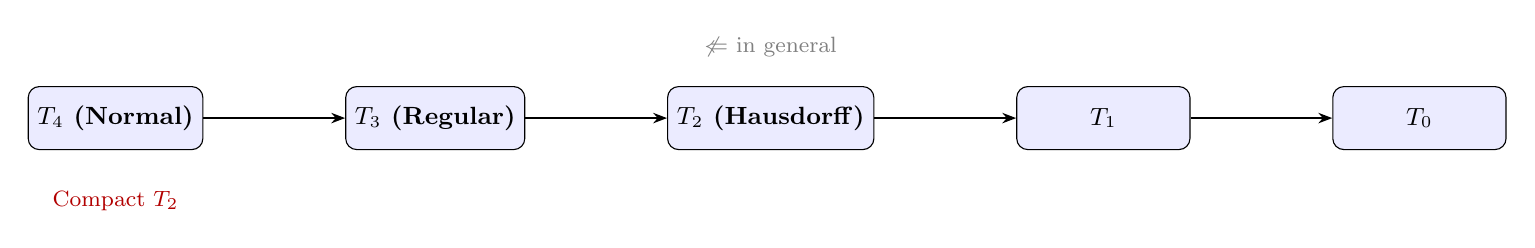
\begin{tikzpicture}[
    axiom/.style={draw, rounded corners, minimum width=2.2cm,
                  minimum height=0.8cm, font=\small\bfseries,
                  fill=blue!8},
    arr/.style={-{Stealth[length=5pt]}, thick},
    node distance=1.8cm
  ]
  \node[axiom] (T4) {$T_4$ (Normal)};
  \node[axiom, right=of T4] (T3) {$T_3$ (Regular)};
  \node[axiom, right=of T3] (T2) {$T_2$ (Hausdorff)};
  \node[axiom, right=of T2] (T1) {$T_1$};
  \node[axiom, right=of T1] (T0) {$T_0$};

  \draw[arr] (T4) -- (T3);
  \draw[arr] (T3) -- (T2);
  \draw[arr] (T2) -- (T1);
  \draw[arr] (T1) -- (T0);

  % Annotations for non-reversals
  \node[below=0.4cm of T4, font=\footnotesize, text=red!70!black]
    {Compact $T_2$};
  \node[above=0.25cm of T2, font=\footnotesize, text=gray]
    {$\not\Leftarrow$ in general};
\end{tikzpicture}
\end{center}

%-------------------------------------------------------------
\section{Counterexamples}
\label{sec:separation-counterexamples}

\begin{example}[Particular point topology: $T_0$ not $T_1$]
\label{ex:particular-point}
\index{particular point topology}
Let $X$ be a set with $|X| \ge 2$ and fix $p \in X$.  Define
$\tau = \{U \subseteq X : p \in U\} \cup \{\varnothing\}$.  For any
$x \neq p$, the open set $\{p\}$ contains $p$ but not $x$, so the space is
$T_0$.  However, if $x \neq p$, every open set containing $x$ must also
contain $p$, so the space is \emph{not} $T_1$.
\end{example}

\begin{example}[Cofinite topology on an infinite set: $T_1$ not $T_2$]
\label{ex:cofinite-not-T2}
\index{cofinite topology!not Hausdorff}
On an infinite set $X$ with the cofinite topology, any two non-empty open sets
$U$ and $V$ satisfy $|X \setminus U| < \infty$ and $|X \setminus V| < \infty$,
so $X \setminus (U \cap V) = (X \setminus U) \cup (X \setminus V)$ is finite.
Since $X$ is infinite, $U \cap V \neq \varnothing$.  Hence no two distinct
points can be separated by disjoint open sets, and the space is not $T_2$.
\end{example}

\begin{example}[$T_2$ but not $T_3$]\label{ex:T2-not-T3}
\index{Hausdorff space!not regular}
Let $X = \mathbb{R}$ with the topology generated by the usual open sets
together with the set $S = \{1/n : n \in \mathbb{N}^*\}$\,.  Formally, a basis
is $\{U \setminus A : U \text{ usual open},\; A \subseteq S\}$.  This is the
\textbf{$K$-topology}\index{K-topology@$K$-topology} on $\mathbb{R}$.  It is
Hausdorff (finer than the usual topology), but the closed set
$F = \{1/n : n \ge 1\}$ (which is closed because its complement
$\mathbb{R} \setminus S$ is open by design) and the point $0 \notin F$ cannot
be separated by disjoint open sets, so the space is not regular.
\end{example}

\begin{example}[The Sorgenfrey plane: $T_3$ not $T_4$]
\label{ex:sorgenfrey-plane}
\index{Sorgenfrey line}\index{Sorgenfrey plane}
The \textbf{Sorgenfrey line} $\mathbb{R}_\ell$ has basis
$\{[a,b) : a < b\}$.  It is $T_4$.  The product
$\mathbb{R}_\ell \times \mathbb{R}_\ell$, the \textbf{Sorgenfrey plane}, is
$T_3$ (products of regular $T_1$ spaces are regular and $T_1$) but \emph{not}
normal.  Indeed, the anti-diagonal
$D = \{(x,-x) : x \in \mathbb{R}\}$ is closed and discrete, and one can show
(using a cardinality argument) that the two disjoint closed subsets
$D_1 = \{(x,-x) : x \in \mathbb{Q}\}$ and
$D_2 = \{(x,-x) : x \in \mathbb{R} \setminus \mathbb{Q}\}$
cannot be separated by disjoint open sets.  (The full proof uses a Baire
category argument on the irrationals.)
\end{example}

%-------------------------------------------------------------
\section{Worked Examples}
\label{sec:separation-worked}

\begin{example}[Subspaces of Hausdorff spaces]\label{ex:subspace-hausdorff}
\textbf{Claim:} Every subspace of a Hausdorff space is Hausdorff.

\textit{Solution.}  Let $Y \subseteq X$ with $X$ Hausdorff, and let
$y_1, y_2 \in Y$ be distinct.  In $X$, there are disjoint open sets
$U_1 \ni y_1$ and $U_2 \ni y_2$.  Then $U_1 \cap Y$ and $U_2 \cap Y$ are
disjoint open sets in $Y$ separating $y_1$ and $y_2$.
\end{example}

\begin{example}[Products of Hausdorff spaces]\label{ex:product-hausdorff}
\textbf{Claim:} An arbitrary product $\prod_{\alpha \in A} X_\alpha$ (with the
product topology) is Hausdorff if and only if each $X_\alpha$ is Hausdorff.

\textit{Solution.}
$(\Rightarrow)$ Each $X_\alpha$ is a continuous image of the product (via the
projection $\pi_\alpha$), and the Hausdorff property passes to subspaces but
not to arbitrary continuous images.  However, each $\pi_\alpha$ is an open map
with a right inverse (fixing a point in every other factor), so $X_\alpha$ is
homeomorphic to a subspace of the product.

$(\Leftarrow)$ Let $(x_\alpha)$ and $(y_\alpha)$ be distinct points.  There
exists $\beta$ with $x_\beta \neq y_\beta$.  Since $X_\beta$ is Hausdorff,
choose disjoint open $U \ni x_\beta$, $V \ni y_\beta$ in $X_\beta$.  Then
$\pi_\beta^{-1}(U)$ and $\pi_\beta^{-1}(V)$ are disjoint open sets in the
product separating the two points.
\end{example}

\begin{example}[The diagonal characterisation of Hausdorff]
\label{ex:diagonal-hausdorff}
\index{Hausdorff space!diagonal characterisation}
\textbf{Claim:} $X$ is Hausdorff if and only if the diagonal
$\Delta = \{(x,x) : x \in X\}$ is closed in $X \times X$.

\textit{Solution.}  $X$ is Hausdorff iff for every $(x,y) \notin \Delta$
(i.e.\ $x \neq y$), there exist open $U \ni x$, $V \ni y$ with
$U \cap V = \varnothing$.  Then $U \times V$ is an open neighbourhood of
$(x,y)$ in $X \times X$ disjoint from $\Delta$.  This holds for all
$(x,y) \notin \Delta$ iff $(X \times X) \setminus \Delta$ is open, i.e.\
$\Delta$ is closed.
\end{example}

\begin{example}[A normal space whose subspace is not normal]
\label{ex:normal-subspace}
\textbf{Claim:} Normality is \emph{not} hereditary.

\textit{Solution.}  The ordinal space $[0, \omega_1]$ with the order topology
is compact Hausdorff, hence normal by Theorem~\ref{thm:compact-hausdorff-normal}.
However, the subspace $[0, \omega_1) \times [0, \omega] \setminus
\{(\omega_1, \omega)\}$ of $[0,\omega_1] \times [0,\omega]$ can be shown to
be Hausdorff but not normal (this is the \emph{Tychonoff plank}%
\index{Tychonoff plank}).
\end{example}

%-------------------------------------------------------------
\section{Exercises}
\label{sec:separation-exercises}

\begin{exercise}[$\bigstar$]\label{exo:T1-finite-hausdorff}
Show that every finite $T_1$ space carries the discrete topology.  Conclude
that a finite topological space is $T_1$ if and only if it is $T_2$.
\end{exercise}

\begin{exercise}[$\bigstar$]\label{exo:hausdorff-convergent-subsequence}
Let $X$ be Hausdorff and let $(x_n)$ be a sequence converging to $x$.  Show
that $\{x\} = \bigcap_{n=1}^\infty \overline{\{x_n, x_{n+1}, \ldots\}}$.
\end{exercise}

\begin{exercise}[$\bigstar$]\label{exo:closed-map-normal}
Let $f \colon X \to Y$ be a continuous, closed, surjective map with $X$ normal.
Prove that $Y$ is normal.
\end{exercise}

\begin{exercise}[$\bigstar\bigstar$]\label{exo:regular-plus-lindelof}
Prove that every regular Lindel\"of space is normal.
\emph{Hint:} mimic the proof of Theorem~\ref{thm:compact-hausdorff-normal},
replacing ``finite subcover'' by ``countable subcover'', then use a
countable shrinking argument.
\end{exercise}

\begin{exercise}[$\bigstar\bigstar$]\label{exo:T1-countable-complement}
Let $X$ be uncountable and let $\tau$ be the \emph{cocountable topology}
(open sets are $\varnothing$ and those with countable complement).  Show that
$X$ is $T_1$ but not $T_2$.
\end{exercise}

\begin{exercise}[$\bigstar\bigstar$]\label{exo:closed-graph}
Let $f \colon X \to Y$ be a function with $Y$ Hausdorff.  Prove that the graph
$\Gamma_f = \{(x, f(x)) : x \in X\}$ is closed in $X \times Y$ if and only if
for every $x \in X$ and every net $(x_\alpha)$ converging to $x$, if
$(f(x_\alpha))$ converges to $y$ then $y = f(x)$.
\end{exercise}

\begin{exercise}[$\bigstar\bigstar$]\label{exo:urysohn-metrization}
Let $X$ be a second-countable $T_3$ space.  Using Urysohn's lemma (which
applies because $X$ is regular Lindel\"of, hence normal by
Exercise~\ref{exo:regular-plus-lindelof}), outline how to embed $X$ into
$[0,1]^{\mathbb{N}}$, thereby showing $X$ is metrizable.
\end{exercise}

\begin{exercise}[$\bigstar\bigstar\bigstar$]\label{exo:jones-lemma}
(\textbf{Jones' Lemma.})\index{Jones' lemma}
Let $X$ be a normal space containing a closed discrete subset $D$ and a dense
subset $S$.  Prove that $2^{|D|} \le 2^{|S|}$.
\emph{Hint:} use Urysohn's lemma to assign to each $A \subseteq D$ a
continuous function $f_A \colon X \to [0,1]$, and show that distinct subsets
give distinct restrictions to $S$.
\end{exercise}

%-------------------------------------------------------------
\section{Chapter Summary}
\label{sec:separation-summary}

\begin{itemize}
\item The separation axioms $T_0$--$T_4$ form a strictly increasing chain of
  topological properties: $T_4 \Rightarrow T_3 \Rightarrow T_2 \Rightarrow
  T_1 \Rightarrow T_0$, with no implication reversing.
\item $T_1$ is equivalent to every singleton being closed.
\item In Hausdorff ($T_2$) spaces, limits of nets are unique and compact
  subsets are closed.
\item Every compact Hausdorff space is normal ($T_4$); every metrizable space
  is normal.
\item Normality is \emph{not} hereditary and \emph{not} productive: the
  Sorgenfrey line is normal, but the Sorgenfrey plane is not.
\item The $K$-topology on $\mathbb{R}$ provides a Hausdorff space that fails
  regularity.
\end{itemize}

\index{separation axioms|)}

%=============================================================
% CHAPTER 6: COMPACTNESS AND TYCHONOFF'S THEOREM
%=============================================================
\chapter{Compactness and Tychonoff's Theorem}\label{ch:compactness}
\index{compactness|(}

Compactness is one of the most powerful and far-reaching concepts in topology.
Its origins lie in analysis: the Heine--Borel theorem asserts that a subset of
$\mathbb{R}^n$ is compact if and only if it is closed and bounded, and the
Bolzano--Weierstrass theorem guarantees that every bounded sequence has a
convergent subsequence.  These results underpin the extreme value theorem,
uniform continuity, and much of the rigorous foundation of calculus.  In
general topology, compactness plays an analogous role: compact spaces behave,
in many ways, like finite sets.  This chapter develops the theory of
compactness from the definition through to Tychonoff's theorem on arbitrary
products, one of the most celebrated results in all of mathematics.

%-------------------------------------------------------------
\section{Definition and First Properties}
\label{sec:compactness-def}

\begin{definition}[Compact space]\label{def:compact}
\index{compact space}
A topological space $X$ is \textbf{compact} if every open cover of $X$ has a
finite subcover.  That is, whenever $\{U_\alpha\}_{\alpha \in A}$ is a
collection of open sets with $X = \bigcup_{\alpha \in A} U_\alpha$, there
exist $\alpha_1, \ldots, \alpha_n \in A$ with
$X = U_{\alpha_1} \cup \cdots \cup U_{\alpha_n}$.

A subset $K$ of a topological space $X$ is \textbf{compact} if $K$ is compact
as a subspace (equivalently, every cover of $K$ by open sets of $X$ has a
finite subcover).
\end{definition}

%-------------------------------------------------------------
\section{The Finite Intersection Property}
\label{sec:FIP}
\index{finite intersection property}

\begin{definition}[Finite intersection property]\label{def:FIP}
A collection $\mathcal{F}$ of subsets of $X$ has the \textbf{finite
intersection property} (FIP) if every finite subcollection has non-empty
intersection:
\[
  F_1, \ldots, F_n \in \mathcal{F} \implies
  F_1 \cap \cdots \cap F_n \neq \varnothing.
\]
\end{definition}

\begin{theorem}[FIP characterisation of compactness]
\label{thm:FIP-compactness}
\index{compactness!FIP characterisation}
A space $X$ is compact if and only if every collection of closed subsets of
$X$ with the finite intersection property has non-empty total intersection.
\end{theorem}

\begin{proof}
This is the contrapositive of the definition, obtained by taking complements.

$(\Rightarrow)$ Let $\{F_\alpha\}_{\alpha \in A}$ be a collection of closed
sets with $\bigcap_\alpha F_\alpha = \varnothing$.  Setting
$U_\alpha = X \setminus F_\alpha$, we have
$\bigcup_\alpha U_\alpha = X$, so $\{U_\alpha\}$ is an open cover.
By compactness, there is a finite subcover:
$X = U_{\alpha_1} \cup \cdots \cup U_{\alpha_n}$.  Taking complements,
$F_{\alpha_1} \cap \cdots \cap F_{\alpha_n} = \varnothing$.  Hence the
collection $\{F_\alpha\}$ does not have the FIP.  Contrapositively, every
collection with the FIP has non-empty intersection.

$(\Leftarrow)$ Given an open cover $\{U_\alpha\}$ with no finite subcover,
the closed sets $F_\alpha = X \setminus U_\alpha$ satisfy
$F_{\alpha_1} \cap \cdots \cap F_{\alpha_n} \neq \varnothing$ for every
finite subcollection (otherwise the corresponding $U_{\alpha_i}$ would cover
$X$).  So $\{F_\alpha\}$ has the FIP, hence
$\bigcap_\alpha F_\alpha \neq \varnothing$, which means
$\bigcup_\alpha U_\alpha \neq X$, contradicting the assumption that
$\{U_\alpha\}$ covers $X$.
\end{proof}

%-------------------------------------------------------------
\section{Fundamental Theorems on Compactness}
\label{sec:compactness-theorems}

\begin{theorem}[Closed subsets of compact spaces]\label{thm:closed-in-compact}
\index{compactness!closed subset}
A closed subset of a compact space is compact.
\end{theorem}

\begin{proof}
Let $X$ be compact, $F \subseteq X$ closed, and let $\{U_\alpha\}$ be an open
cover of $F$ (by open sets of $X$).  Then
$\{U_\alpha\} \cup \{X \setminus F\}$ is an open cover of $X$.  By
compactness of $X$, a finite subcollection covers $X$:
\[
  X = U_{\alpha_1} \cup \cdots \cup U_{\alpha_n} \cup (X \setminus F).
\]
Then $F \subseteq U_{\alpha_1} \cup \cdots \cup U_{\alpha_n}$.
\end{proof}

\begin{theorem}[Compact subsets of Hausdorff spaces are closed]
\label{thm:compact-hausdorff-closed}
\index{compactness!in Hausdorff space}
If $X$ is Hausdorff and $K \subseteq X$ is compact, then $K$ is closed.
\end{theorem}

\begin{proof}
This was proved as Theorem~\ref{thm:compact-in-hausdorff-closed} in
Chapter~\ref{ch:separation-axioms}.
\end{proof}

\begin{theorem}[Continuous image of a compact space]
\label{thm:continuous-image-compact}
\index{compactness!continuous image}
If $f \colon X \to Y$ is continuous and $X$ is compact, then $f(X)$ is
compact.
\end{theorem}

\begin{proof}
Let $\{V_\alpha\}$ be an open cover of $f(X)$.  Then
$\{f^{-1}(V_\alpha)\}$ is an open cover of $X$ (by continuity).
Compactness of $X$ yields a finite subcover
$X = f^{-1}(V_{\alpha_1}) \cup \cdots \cup f^{-1}(V_{\alpha_n})$.
Applying $f$,
\[
  f(X) \subseteq V_{\alpha_1} \cup \cdots \cup V_{\alpha_n}. \qedhere
\]
\end{proof}

\begin{corollary}[Extreme value theorem]\label{cor:extreme-value}
\index{extreme value theorem}
If $X$ is compact and $f \colon X \to \mathbb{R}$ is continuous, then $f$
attains its maximum and minimum on $X$.
\end{corollary}

\begin{proof}
By Theorem~\ref{thm:continuous-image-compact}, $f(X)$ is a compact subset of
$\mathbb{R}$.  By the Heine--Borel theorem (Theorem~\ref{thm:heine-borel}
below, or its classical form), $f(X)$ is closed and bounded.  A closed bounded
subset of $\mathbb{R}$ contains its supremum and infimum.
\end{proof}

%-------------------------------------------------------------
\section{Compactness in \texorpdfstring{$\mathbb{R}^n$}{Rn}}
\label{sec:compactness-Rn}

\begin{theorem}[{Compactness of $[a,b]$}]\label{thm:closed-interval-compact}
\index{compactness!of $[a,b]$}
Every closed bounded interval $[a,b] \subseteq \mathbb{R}$ is compact.
\end{theorem}

\begin{proof}
Let $\mathcal{U} = \{U_\alpha\}_{\alpha \in A}$ be an open cover of $[a,b]$.
Define
\[
  S = \bigl\{\, s \in [a,b] : [a,s] \text{ is covered by finitely many
    members of } \mathcal{U} \,\bigr\}.
\]
The set $S$ is non-empty ($a$ belongs to some $U_\alpha$, and for $s$
sufficiently close to $a$ we have $[a,s] \subseteq U_\alpha$, so $s \in S$).
Since $S \subseteq [a,b]$, $S$ is bounded above and we set $c = \sup S$.

\emph{Claim: $c \in S$.}
Choose $U_\beta \ni c$.  Since $U_\beta$ is open in $[a,b]$, there exists
$\varepsilon > 0$ with $(c - \varepsilon, c] \cap [a,b] \subseteq U_\beta$.
By the definition of supremum, there exists $s \in S$ with
$s > c - \varepsilon$.  Then $[a,s]$ is covered by finitely many members
of $\mathcal{U}$, and $[s, c] \subseteq U_\beta$, so $[a,c]$ is covered by
finitely many members of $\mathcal{U}$.  Hence $c \in S$.

\emph{Claim: $c = b$.}
Suppose $c < b$.  The open set $U_\beta \ni c$ contains an interval
$[c, c + \delta)$ for some $\delta > 0$ (taking $\delta$ small enough that
$c + \delta \le b$).  Then $[a, c + \delta/2]$ is covered by the finite
subcover of $[a,c]$ together with $U_\beta$, contradicting
$c = \sup S$.

Therefore $c = b \in S$, and $[a,b]$ has a finite subcover.
\end{proof}

\begin{theorem}[Heine--Borel]\label{thm:heine-borel}
\index{Heine--Borel theorem}
A subset of $\mathbb{R}^n$ is compact if and only if it is closed and bounded.
\end{theorem}

\begin{proof}
$(\Leftarrow)$ A closed bounded subset $K \subseteq \mathbb{R}^n$ is contained
in some box $[-M,M]^n$.  By Theorem~\ref{thm:closed-interval-compact},
$[-M,M]$ is compact.  By Tychonoff's theorem
(Theorem~\ref{thm:tychonoff} below, or by an elementary induction on $n$),
the finite product $[-M,M]^n$ is compact.  Since $K$ is a closed subset of a
compact space, $K$ is compact by Theorem~\ref{thm:closed-in-compact}.

$(\Rightarrow)$ A compact subset of a Hausdorff space is closed
(Theorem~\ref{thm:compact-hausdorff-closed}).  To see it is bounded, the
open cover $\{B(0,n)\}_{n=1}^\infty$ of $K$ has a finite subcover, so
$K \subseteq B(0,N)$ for some $N$.
\end{proof}

%-------------------------------------------------------------
\section{Sequential and Limit Point Compactness}
\label{sec:sequential-compactness}
\index{sequential compactness}\index{limit point compactness}

\begin{definition}\label{def:sequential-compact}
A space $X$ is \textbf{sequentially compact} if every sequence in $X$ has a
convergent subsequence.
\end{definition}

\begin{definition}\label{def:limit-point-compact}
A space $X$ is \textbf{limit point compact} (or \textbf{Bolzano--Weierstrass})
if every infinite subset of $X$ has a limit point (accumulation point) in $X$.
\end{definition}

\begin{proposition}\label{prop:compact-implies-lpc}
Compact $\Rightarrow$ limit point compact.
\end{proposition}

\begin{proof}
Suppose $X$ is compact and $A \subseteq X$ is infinite with no limit point.
Then $A$ is closed (its complement is open since no point outside $A$ is a
limit point).  For each $a \in A$, there is an open set $U_a$ with
$U_a \cap A = \{a\}$.  Then $\{U_a\}_{a \in A} \cup \{X \setminus A\}$ is an
open cover of $X$ with no finite subcover (since $A$ is infinite), contradicting
compactness.
\end{proof}

\begin{theorem}[Equivalence in metric spaces]\label{thm:metric-compactness}
\index{compactness!in metric spaces}
For a metric space $(X,d)$, the following are equivalent:
\begin{enumerate}
\item $X$ is compact.
\item $X$ is sequentially compact.
\item $X$ is complete and totally bounded.
\end{enumerate}
\end{theorem}

\begin{proof}
\emph{$(1) \Rightarrow (2)$:}
Compact implies limit point compact (Proposition~\ref{prop:compact-implies-lpc}).
In a metric space (which is first countable), limit point compactness implies
sequential compactness.  Indeed, if $(x_n)$ is a sequence and
$A = \{x_n : n \in \mathbb{N}\}$ is finite, then some value repeats infinitely
often, giving a (constant, hence convergent) subsequence.  If $A$ is infinite,
it has a limit point $p$; since $X$ is first countable, we can extract a
subsequence converging to $p$.

\emph{$(2) \Rightarrow (3)$:}
\textit{Completeness:}  Every Cauchy sequence in a sequentially compact space
has a convergent subsequence, and a Cauchy sequence with a convergent
subsequence converges.

\textit{Total boundedness:}  Suppose $X$ is not totally bounded.  Then there
exists $\varepsilon > 0$ such that no finite set of $\varepsilon$-balls covers
$X$.  Inductively choose $x_1 \in X$, and given $x_1, \ldots, x_n$, choose
$x_{n+1} \notin \bigcup_{i=1}^n B(x_i, \varepsilon)$.  The sequence $(x_n)$
satisfies $d(x_m, x_n) \ge \varepsilon$ for all $m \neq n$, so it has no
convergent subsequence, contradicting sequential compactness.

\emph{$(3) \Rightarrow (1)$:}
Let $\{U_\alpha\}$ be an open cover with no finite subcover.  Since $X$ is
totally bounded, cover $X$ by finitely many balls of radius $1$.  At least one,
say $B_1$, cannot be covered by finitely many $U_\alpha$.  The closure
$\overline{B_1}$ is totally bounded; cover it by finitely many balls of radius
$1/2$.  At least one, say $B_2$, cannot be finitely covered.  Continue
inductively with radii $1/n$ to obtain a nested sequence of sets
$\overline{B_n}$ with $\operatorname{diam}(\overline{B_n}) \le 2/n$.  Pick
$x_n \in \overline{B_n}$.  Then $(x_n)$ is Cauchy; by completeness,
$x_n \to x$ for some $x \in X$.  Choose $U_\beta \ni x$.  For large $n$,
$\overline{B_n} \subseteq U_\beta$ (since $\operatorname{diam}(\overline{B_n})
\to 0$ and $x_n \to x$).  But then $\overline{B_n}$ is covered by a single
$U_\beta$, contradicting the choice of $B_n$.
\end{proof}

%-------------------------------------------------------------
\section{Alexander's Sub-base Theorem}
\label{sec:alexander}
\index{Alexander's sub-base theorem}

\begin{theorem}[Alexander's sub-base theorem]\label{thm:alexander}
Let $\mathcal{S}$ be a sub-base for the topology on $X$.  If every cover of
$X$ by members of $\mathcal{S}$ has a finite subcover, then $X$ is compact.
\end{theorem}

\begin{proof}
We prove the contrapositive.  Suppose $X$ is not compact.  We must find a cover
by sub-basic open sets with no finite subcover.

Consider the collection $\Sigma$ of all open covers of $X$ that have no finite
subcover.  By assumption, $\Sigma \neq \varnothing$.  Order $\Sigma$ by
inclusion: $\mathcal{U} \le \mathcal{V}$ if $\mathcal{U} \subseteq
\mathcal{V}$.  We apply Zorn's lemma.

\emph{Chain condition:}  Let $\{\mathcal{U}_i\}_{i \in I}$ be a chain in
$\Sigma$.  Set $\mathcal{U} = \bigcup_{i \in I} \mathcal{U}_i$.  This is a
collection of open sets covering $X$ (since each $\mathcal{U}_i$ covers $X$).
If $\mathcal{U}$ had a finite subcover $\{V_1, \ldots, V_k\}$, then each
$V_j \in \mathcal{U}_{i_j}$ for some $i_j$.  Since the chain is totally
ordered, there exists $i_0$ with $\mathcal{U}_{i_j} \subseteq
\mathcal{U}_{i_0}$ for all $j$, so $\{V_1, \ldots, V_k\} \subseteq
\mathcal{U}_{i_0}$, contradicting $\mathcal{U}_{i_0} \in \Sigma$.  Hence
$\mathcal{U} \in \Sigma$, and $\mathcal{U}$ is an upper bound for the chain.

By Zorn's lemma, $\Sigma$ has a maximal element $\mathcal{M}$.  Thus
$\mathcal{M}$ is an open cover of $X$ with no finite subcover, and it is
maximal with respect to this property (adding any open set not in $\mathcal{M}$
creates a cover admitting a finite subcover).

\emph{Claim:} $\mathcal{M} \cap \mathcal{S}$ already covers $X$.

Suppose not.  Then there exists $x \in X$ not covered by any member of
$\mathcal{M} \cap \mathcal{S}$.  Since $\mathcal{M}$ covers $X$, there exists
$U \in \mathcal{M}$ with $x \in U$.  Since $\mathcal{S}$ is a sub-base, $U$
contains a basic open set $S_1 \cap \cdots \cap S_m$ with $x \in S_1 \cap
\cdots \cap S_m$ and each $S_j \in \mathcal{S}$.  Since $x$ is not covered by
$\mathcal{M} \cap \mathcal{S}$, for each $j$ we have $S_j \notin \mathcal{M}$.

By the maximality of $\mathcal{M}$, for each $j$ the cover
$\mathcal{M} \cup \{S_j\}$ admits a finite subcover.  Hence there exist
$M_{j,1}, \ldots, M_{j, k_j} \in \mathcal{M}$ such that
\[
  X = S_j \cup M_{j,1} \cup \cdots \cup M_{j, k_j}.
\]
Now consider $x \in S_1 \cap \cdots \cap S_m \subseteq U$.  We have
\[
  X = \bigcap_{j=1}^m \bigl(S_j \cup M_{j,1} \cup \cdots \cup
  M_{j,k_j}\bigr).
\]
For any point $p \in X$:  if $p \in S_j$ for all $j$, then
$p \in S_1 \cap \cdots \cap S_m \subseteq U \in \mathcal{M}$.  Otherwise
$p \notin S_j$ for some $j$, so $p \in M_{j,1} \cup \cdots \cup M_{j,k_j}$.
In either case, $p$ is covered by $\{U\} \cup \bigcup_{j=1}^m
\{M_{j,1}, \ldots, M_{j,k_j}\}$, which is a finite subcollection of
$\mathcal{M}$.  This contradicts $\mathcal{M} \in \Sigma$.

Hence $\mathcal{M} \cap \mathcal{S}$ covers $X$, and it has no finite subcover
(since $\mathcal{M}$ does not).  Therefore we have found a sub-basic cover with
no finite subcover.
\end{proof}

%-------------------------------------------------------------
\section{Tychonoff's Theorem}
\label{sec:tychonoff}
\index{Tychonoff's theorem}

\begin{theorem}[Tychonoff]\label{thm:tychonoff}
Let $\{X_\alpha\}_{\alpha \in A}$ be a (possibly infinite) collection of
non-empty topological spaces.  Then the product
$X = \prod_{\alpha \in A} X_\alpha$ (with the product topology) is compact if
and only if each $X_\alpha$ is compact.
\end{theorem}

\begin{proof}
$(\Rightarrow)$ Each projection $\pi_\alpha \colon X \to X_\alpha$ is
continuous and surjective.  By Theorem~\ref{thm:continuous-image-compact}, if
$X$ is compact then each $X_\alpha = \pi_\alpha(X)$ is compact.

$(\Leftarrow)$ Assume each $X_\alpha$ is compact.  We use Alexander's sub-base
theorem (Theorem~\ref{thm:alexander}).

Recall that the product topology has a sub-base
\[
  \mathcal{S} = \bigl\{\, \pi_\alpha^{-1}(U_\alpha) :
    \alpha \in A,\; U_\alpha \subseteq X_\alpha \text{ open} \,\bigr\}.
\]
By Alexander's theorem, it suffices to show that every cover of $X$ by members
of $\mathcal{S}$ has a finite subcover.

Let $\mathcal{C} \subseteq \mathcal{S}$ be a cover of $X$ with no finite
subcover.  For each $\alpha \in A$, define
\[
  \mathcal{C}_\alpha = \bigl\{\, U_\alpha \subseteq X_\alpha :
    \pi_\alpha^{-1}(U_\alpha) \in \mathcal{C} \,\bigr\}.
\]
\emph{Claim: for each $\alpha$, $\mathcal{C}_\alpha$ does not cover
$X_\alpha$.}

Suppose $\mathcal{C}_\alpha$ covers $X_\alpha$ for some $\alpha$.  Since
$X_\alpha$ is compact, there exist $U_{\alpha,1}, \ldots, U_{\alpha,n}
\in \mathcal{C}_\alpha$ with
$X_\alpha = U_{\alpha,1} \cup \cdots \cup U_{\alpha,n}$.  Then
\[
  X = \pi_\alpha^{-1}(X_\alpha) = \pi_\alpha^{-1}(U_{\alpha,1})
  \cup \cdots \cup \pi_\alpha^{-1}(U_{\alpha,n}),
\]
which is a finite subcover of $\mathcal{C}$, contradicting our assumption.

So for each $\alpha \in A$, there exists $x_\alpha \in X_\alpha$ with
$x_\alpha \notin \bigcup \mathcal{C}_\alpha$.  Define $x = (x_\alpha)_{\alpha
\in A} \in X$.

Since $\mathcal{C}$ covers $X$, there exists $\pi_\beta^{-1}(U_\beta) \in
\mathcal{C}$ with $x \in \pi_\beta^{-1}(U_\beta)$.  This means
$x_\beta = \pi_\beta(x) \in U_\beta$, so $U_\beta \in \mathcal{C}_\beta$,
contradicting the choice $x_\beta \notin \bigcup \mathcal{C}_\beta$.

The contradiction shows that no such cover $\mathcal{C}$ exists, so every
sub-basic cover has a finite subcover.  By Alexander's theorem, $X$ is compact.
\end{proof}

\begin{remark}\label{rem:tychonoff-ac}
The proof of Tychonoff's theorem uses the Axiom of Choice (via Zorn's lemma
in Alexander's sub-base theorem, and also in selecting the points
$x_\alpha$).  In fact, Tychonoff's theorem is \emph{equivalent} to the Axiom
of Choice in ZF, as proved by Kelley (1950).
\end{remark}

%-------------------------------------------------------------
\section{The Alexandroff One-Point Compactification}
\label{sec:alexandroff}
\index{Alexandroff compactification}\index{one-point compactification}

\begin{definition}[One-point compactification]\label{def:one-point-compact}
Let $X$ be a non-compact, locally compact, Hausdorff topological space.  The
\textbf{one-point (Alexandroff) compactification} of $X$ is the space
$X^* = X \cup \{\infty\}$ (where $\infty \notin X$) with the topology
\[
  \tau^* = \tau \cup \bigl\{\, (X \setminus K) \cup \{\infty\} :
    K \subseteq X \text{ compact} \,\bigr\}.
\]
\end{definition}

\begin{proposition}\label{prop:alexandroff-properties}
The space $X^*$ is compact and Hausdorff, $X$ embeds as an open dense subspace,
and the topology $\tau^*$ is the unique compact Hausdorff topology on
$X \cup \{\infty\}$ that restricts to $\tau$ on $X$.
\end{proposition}

\begin{proof}
\emph{$\tau^*$ is a topology.}  The empty set and $X^*$ are in $\tau^*$
($\varnothing \in \tau$ and $X^* = (X \setminus \varnothing) \cup \{\infty\}$
with $\varnothing$ compact).  Unions and finite intersections of sets in
$\tau^*$ remain in $\tau^*$: for sets not containing $\infty$ this follows from
$\tau$ being a topology; for sets containing $\infty$, it follows from the fact
that finite unions of compact sets are compact and arbitrary intersections of
compact (closed) sets in a Hausdorff space are compact (closed).

\emph{Compactness.}
Let $\{V_\beta\}$ be an open cover of $X^*$.  Some $V_{\beta_0}$ contains
$\infty$, so $V_{\beta_0} = (X \setminus K) \cup \{\infty\}$ for some compact
$K \subseteq X$.  The remaining sets $\{V_\beta\}_{\beta \neq \beta_0}$ (intersected
with $X$) cover $K$.  By compactness of $K$, finitely many suffice.  Adding
$V_{\beta_0}$ gives a finite subcover of $X^*$.

\emph{Hausdorff.}
Two points in $X$ are separated because $X$ is Hausdorff.  For $x \in X$ and
$\infty$:  by local compactness, there is an open $U \ni x$ with $\overline{U}$
compact.  Then $U$ and $(X \setminus \overline{U}) \cup \{\infty\}$ are
disjoint open sets separating $x$ and $\infty$.
\end{proof}

\begin{example}[$\mathbb{R} \cup \{\infty\} \cong S^1$]
\label{ex:one-point-R}
\index{Alexandroff compactification!of $\mathbb{R}$}
The one-point compactification of $\mathbb{R}$ is homeomorphic to the circle
$S^1$.  A homeomorphism is given by stereographic projection from the
``north pole'' of $S^1$: the map sends each $t \in \mathbb{R}$ to the
corresponding point on $S^1 \setminus \{N\}$ and $\infty$ to $N$.
\end{example}

\begin{example}[$\mathbb{C} \cup \{\infty\} \cong S^2$]
\label{ex:one-point-C}
\index{Alexandroff compactification!of $\mathbb{C}$}
Similarly, the one-point compactification of $\mathbb{C} \cong \mathbb{R}^2$
is the \textbf{Riemann sphere}\index{Riemann sphere} $S^2$, via stereographic
projection.
\end{example}

The following TikZ diagram illustrates the one-point compactification of the
real line.

\begin{center}
\begin{tikzpicture}[scale=1.2]
  % The real line
  \draw[thick, ->] (-3.5,0) -- (3.5,0) node[right] {$\mathbb{R}$};
  \foreach \x in {-3,-2,-1,0,1,2,3}
    \draw (\x, 0.07) -- (\x, -0.07) node[below, font=\footnotesize] {$\x$};

  % The circle (compactification)
  \draw[thick] (0,2.5) circle (1.2);
  \fill (0,3.7) circle (1.5pt) node[above] {$\infty$};
  \node at (0,2.5) [font=\footnotesize] {$S^1$};

  % Arrows indicating the compactification
  \draw[->, dashed, gray] (-2.5, 0.3) to[out=90, in=200] (-0.9, 1.6);
  \draw[->, dashed, gray] (2.5, 0.3) to[out=90, in=-20] (0.9, 1.6);
  \draw[->, dashed, gray] (0, 0.3) to[out=90, in=-90] (0, 1.3);
\end{tikzpicture}
\end{center}

%-------------------------------------------------------------
\section{The Stone--\v{C}ech Compactification}
\label{sec:stone-cech}
\index{Stone--Cech compactification@Stone--\v{C}ech compactification}

While the Alexandroff compactification adds a single point, the
\textbf{Stone--\v{C}ech compactification} $\beta X$ is in a precise sense the
``largest'' compactification of a completely regular ($T_{3\frac{1}{2}}$) space
$X$.  It is characterised by the universal property: every continuous function
$f \colon X \to K$ into a compact Hausdorff space $K$ extends uniquely to a
continuous function $\tilde{f} \colon \beta X \to K$.  The construction can be
carried out by embedding $X$ into a product of copies of $[0,1]$ (one for each
bounded continuous function $X \to [0,1]$) and taking the closure; Tychonoff's
theorem guarantees compactness of the ambient product.  A detailed treatment
lies beyond our scope, but the interested reader is referred to
Engelking~\cite{engelking1989} or Willard~\cite{willard}.

%-------------------------------------------------------------
\section{Visualisation: Open Covers}
\label{sec:open-cover-tikz}

\begin{center}
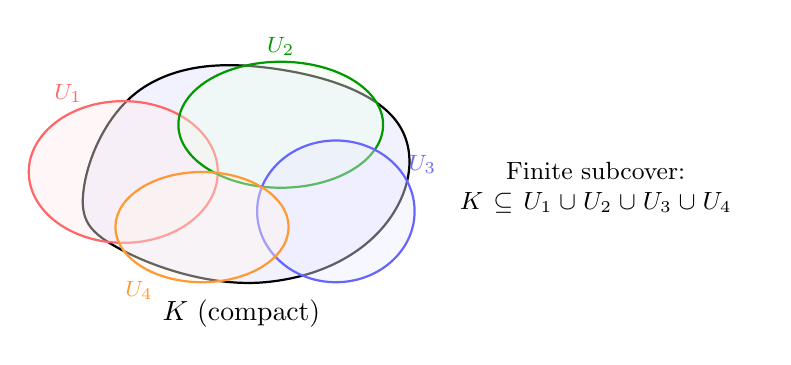
\begin{tikzpicture}
  % A compact set
  \draw[thick, fill=blue!5] plot[smooth cycle, tension=0.7]
    coordinates {(-2,0) (-1.2,1.3) (0.5,1.5) (2,0.8) (1.8,-0.5)
    (0.3,-1.2) (-1.5,-0.8)};
  \node at (0,-1.6) {$K$ (compact)};

  % Open cover sets
  \draw[red!60, thick, fill=red!8, fill opacity=0.4]
    (-1.5,0.2) ellipse (1.2 and 0.9);
  \draw[green!60!black, thick, fill=green!8, fill opacity=0.4]
    (0.5,0.8) ellipse (1.3 and 0.8);
  \draw[blue!60, thick, fill=blue!8, fill opacity=0.4]
    (1.2,-0.3) ellipse (1.0 and 0.9);
  \draw[orange!80, thick, fill=orange!8, fill opacity=0.4]
    (-0.5,-0.5) ellipse (1.1 and 0.7);

  \node[red!60, font=\footnotesize] at (-2.2, 1.2) {$U_1$};
  \node[green!60!black, font=\footnotesize] at (0.5, 1.8) {$U_2$};
  \node[blue!60, font=\footnotesize] at (2.3, 0.3) {$U_3$};
  \node[orange!80, font=\footnotesize] at (-1.3, -1.3) {$U_4$};

  \node[font=\small, text width=4cm, align=center] at (4.5, 0)
    {Finite subcover:\\$K \subseteq U_1 \cup U_2 \cup U_3 \cup U_4$};
\end{tikzpicture}
\end{center}

%-------------------------------------------------------------
\section{Counterexamples}
\label{sec:compactness-counterexamples}

\begin{example}[$(0,1)$ is not compact]\label{ex:open-interval-not-compact}
\index{compactness!counterexamples}
The open interval $(0,1)$ is not compact.  The open cover
$\{(1/n, 1) : n \ge 2\}$ has no finite subcover: any finite subcollection
misses points near $0$.
\end{example}

\begin{example}[{$\mathbb{Q} \cap {[0,1]}$ is not compact}]
\label{ex:rationals-not-compact}
The space $\mathbb{Q} \cap [0,1]$ (with the subspace topology from
$\mathbb{R}$) is not compact.  Choose an irrational $r \in (0,1)$ (say
$r = 1/\sqrt{2}$) and consider the open cover
$\{[0, r - 1/n) \cup (r + 1/n, 1] : n \ge 1\} \cap \mathbb{Q}$;
no finite subcover exists.  Alternatively, $\mathbb{Q} \cap [0,1]$ is not
closed in $\mathbb{R}$, yet is bounded, so by the Heine--Borel theorem it
cannot be compact (as a subset of $\mathbb{R}$).
\end{example}

\begin{example}[Sequential compactness $\neq$ compactness in general]
\label{ex:seq-compact-neq-compact}
\index{sequential compactness!vs compactness}
The product $\{0,1\}^{[0,1]}$ (with the product topology, where $\{0,1\}$ is
discrete) is compact by Tychonoff's theorem.  However, the subspace
$\omega_1 = [0, \omega_1)$ with the order topology is sequentially compact
(every sequence of countable ordinals is bounded by a countable ordinal and
hence has a convergent subsequence) but not compact (the open cover
$\{[0,\alpha) : \alpha < \omega_1\}$ has no finite subcover).

Conversely, the product $\{0,1\}^{\mathbb{R}}$ is compact (Tychonoff) but
not sequentially compact.  These examples show that compactness and
sequential compactness are genuinely distinct in general topological spaces.
\end{example}

%-------------------------------------------------------------
\section{Worked Examples}
\label{sec:compactness-worked}

\begin{example}[Continuous bijection from compact to Hausdorff is a
  homeomorphism]\label{ex:compact-to-hausdorff-homeo}
\index{homeomorphism!compact to Hausdorff}
\textbf{Claim:} If $f \colon X \to Y$ is a continuous bijection, $X$ is
compact, and $Y$ is Hausdorff, then $f$ is a homeomorphism.

\textit{Solution.}  It suffices to show $f$ is a closed map.  Let
$F \subseteq X$ be closed.  Since $X$ is compact and $F$ is closed, $F$ is
compact (Theorem~\ref{thm:closed-in-compact}).  Then $f(F)$ is compact
(Theorem~\ref{thm:continuous-image-compact}).  Since $Y$ is Hausdorff, $f(F)$
is closed (Theorem~\ref{thm:compact-hausdorff-closed}).  Hence $f$ is closed,
and a continuous closed bijection is a homeomorphism.
\end{example}

\begin{example}[Compactness of the Cantor set]\label{ex:cantor-compact}
\index{Cantor set!compactness}
\textbf{Claim:} The Cantor set $C \subseteq [0,1]$ is compact.

\textit{Solution.}  The Cantor set is constructed as
$C = \bigcap_{n=0}^\infty C_n$ where each $C_n$ is a finite union of closed
intervals (hence closed).  Thus $C$ is an intersection of closed sets in
$[0,1]$, hence closed in $[0,1]$.  Since $[0,1]$ is compact
(Theorem~\ref{thm:closed-interval-compact}) and $C$ is a closed subset, $C$ is
compact by Theorem~\ref{thm:closed-in-compact}.

Alternatively, $C$ is homeomorphic to $\{0,1\}^{\mathbb{N}}$ (via the ternary
expansion), which is compact by Tychonoff's theorem.
\end{example}

\begin{example}[{The product of ${[0,1]}$ with itself uncountably many times}]
\label{ex:hilbert-cube-general}
\index{Tychonoff's theorem!application}
\textbf{Claim:} For any index set $A$, the product $[0,1]^A$ is compact.

\textit{Solution.}  Each factor $[0,1]$ is compact (being a closed bounded
interval in $\mathbb{R}$).  By Tychonoff's theorem
(Theorem~\ref{thm:tychonoff}), the arbitrary product $[0,1]^A$ is compact.
When $A = \mathbb{N}$, this gives the \textbf{Hilbert cube}\index{Hilbert cube}
$[0,1]^{\mathbb{N}}$, a fundamental object in infinite-dimensional topology.
\end{example}

\begin{example}[Tube lemma application]\label{ex:tube-lemma}
\index{tube lemma}
\textbf{Claim (Tube Lemma):} If $X$ is compact and $Y$ is any space, $x_0 \in X$,
and $N$ is an open set in $X \times Y$ containing the ``slice''
$X \times \{y_0\}$, then there exists an open set $V \ni y_0$ in $Y$ such that
$X \times V \subseteq N$.

\textit{Solution.}  For each $x \in X$, the point $(x, y_0) \in N$, so there
exist open sets $U_x \ni x$ and $V_x \ni y_0$ in $X$ and $Y$ respectively with
$U_x \times V_x \subseteq N$.  The sets $\{U_x\}_{x \in X}$ cover the compact
space $X$, so finitely many suffice: $X = U_{x_1} \cup \cdots \cup U_{x_n}$.
Set $V = V_{x_1} \cap \cdots \cap V_{x_n}$.  Then $V$ is open, $y_0 \in V$,
and $X \times V \subseteq N$.
\end{example}

%-------------------------------------------------------------
\section{Exercises}
\label{sec:compactness-exercises}

\begin{exercise}[$\bigstar$]\label{exo:compact-discrete}
Prove that a discrete topological space is compact if and only if it is finite.
\end{exercise}

\begin{exercise}[$\bigstar$]\label{exo:compact-intersection}
Let $X$ be a compact space and let $\{F_n\}_{n \ge 1}$ be a decreasing
sequence of non-empty closed subsets ($F_1 \supseteq F_2 \supseteq \cdots$).
Prove that $\bigcap_{n=1}^\infty F_n \neq \varnothing$.
\end{exercise}

\begin{exercise}[$\bigstar$]\label{exo:compact-metric-bounded}
Show that every compact metric space is bounded, and that every compact metric
space is complete.
\end{exercise}

\begin{exercise}[$\bigstar\bigstar$]\label{exo:lebesgue-number}
(\textbf{Lebesgue number lemma.})\index{Lebesgue number lemma}
Let $(X,d)$ be a compact metric space and $\{U_\alpha\}$ an open cover.
Prove there exists $\delta > 0$ (the \emph{Lebesgue number}) such that every
subset of $X$ with diameter less than $\delta$ is contained in some
$U_\alpha$.
\end{exercise}

\begin{exercise}[$\bigstar\bigstar$]\label{exo:compact-hausdorff-homeo}
Let $X$ be compact, $Y$ Hausdorff, and $f \colon X \to Y$ a continuous
bijection.  Prove $f$ is a homeomorphism.
(This generalises Example~\ref{ex:compact-to-hausdorff-homeo}; give a
complete proof.)
\end{exercise}

\begin{exercise}[$\bigstar\bigstar$]\label{exo:compact-product-finite}
Without using Tychonoff's theorem, prove directly that if $X$ and $Y$ are
compact, then $X \times Y$ is compact.
\emph{Hint:} use the tube lemma (Example~\ref{ex:tube-lemma}).
\end{exercise}

\begin{exercise}[$\bigstar\bigstar$]\label{exo:one-point-compact-characterise}
Let $X$ be a locally compact Hausdorff space.  Show that the one-point
compactification $X^*$ is (up to homeomorphism) the unique compact Hausdorff
space containing $X$ as an open dense subspace.
\end{exercise}

\begin{exercise}[$\bigstar\bigstar\bigstar$]\label{exo:tychonoff-equiv-ac}
Show that Tychonoff's theorem implies the Axiom of Choice.
\emph{Hint:} Given a family $\{X_\alpha\}_{\alpha \in A}$ of non-empty sets,
consider $Y_\alpha = X_\alpha \cup \{\star\}$ with the topology
$\{\varnothing, X_\alpha, Y_\alpha\}$, show each $Y_\alpha$ is compact, and
use Tychonoff to find a point in $\prod X_\alpha$.
\end{exercise}

\begin{exercise}[$\bigstar\bigstar\bigstar$]\label{exo:baire-compact}
(\textbf{Baire category theorem for compact Hausdorff spaces.})%
\index{Baire category theorem}
Prove that in a compact Hausdorff space, the intersection of countably many
dense open sets is dense.
\emph{Hint:} given a non-empty open $W$, inductively construct a nested
sequence of open sets $U_1 \supseteq \overline{U_2} \supseteq U_2 \supseteq
\cdots$ with $\overline{U_n}$ compact and $\overline{U_n} \subseteq G_n \cap W$,
then use the FIP.
\end{exercise}

%-------------------------------------------------------------
\section{Chapter Summary}
\label{sec:compactness-summary}

\begin{itemize}
\item A space is compact if every open cover has a finite subcover;
  equivalently, every collection of closed sets with the FIP has non-empty
  intersection.
\item Closed subsets of compact spaces are compact; compact subsets of
  Hausdorff spaces are closed; continuous images of compact spaces are compact.
\item The extreme value theorem is a corollary: continuous real-valued functions
  on compact spaces attain their bounds.
\item $[a,b]$ is compact (direct proof via the least upper bound property),
  and the Heine--Borel theorem characterises compact subsets of $\mathbb{R}^n$
  as the closed and bounded sets.
\item In metric spaces, compactness is equivalent to sequential compactness and
  to completeness plus total boundedness.  In general spaces, these notions
  diverge.
\item Alexander's sub-base theorem reduces checking compactness to sub-basic
  covers; this is the key tool in proving Tychonoff's theorem.
\item \textbf{Tychonoff's theorem}: an arbitrary product of compact spaces is
  compact (in the product topology).  This result is equivalent to the Axiom
  of Choice.
\item The Alexandroff one-point compactification adds a single point to a
  locally compact Hausdorff space; the Stone--\v{C}ech compactification
  provides the ``maximal'' compactification.
\end{itemize}

\index{compactness|)}
%%%%%%%%%%%%%%%%%%%%%%%%%%%%%%%%%%%%%%%%%%%%%%%%%%%%%%%%%%%%%
%  PART 4 — Chapters 7 & 8
%  General Topology: Connectedness, Products, Quotients
%%%%%%%%%%%%%%%%%%%%%%%%%%%%%%%%%%%%%%%%%%%%%%%%%%%%%%%%%%%%%

%%%%%%%%%%%%%%%%%%%%%%%%%%%%%%%%%%%%%%%%%%%%%%%%%%%%%%%%%%%%%
\chapter{Connectedness and Path-Connectedness}\label{ch:connectedness}
\index{connectedness|(}
%%%%%%%%%%%%%%%%%%%%%%%%%%%%%%%%%%%%%%%%%%%%%%%%%%%%%%%%%%%%%

One of the most intuitive topological properties is that of being
``in one piece.''  In analysis on the real line, this idea is captured
by the classical result that the connected subsets of~$\mathbb{R}$
are precisely the intervals (bounded or unbounded, open, closed,
or half-open).  The goal of this chapter is to formalize and extend
this notion to arbitrary topological spaces.  We shall meet two
flavors of the concept---\emph{connectedness} and
\emph{path-connectedness}---study their interplay, and exhibit
spaces that separate the two notions.

%----------------------------------------------------------
\section{Connected Spaces}\label{sec:connected-spaces}
\index{connected space}
%----------------------------------------------------------

\begin{definition}[Separation]\label{def:separation}
\index{separation}
Let $X$ be a topological space.  A \textbf{separation} of $X$ is
a pair $(U,V)$ of non-empty open subsets $U,V\subseteq X$ such that
\[
   U\cap V=\varnothing \quad\text{and}\quad U\cup V=X.
\]
The space $X$ is called \textbf{disconnected}\index{disconnected space}
if it admits a separation, and \textbf{connected}\index{connected space}
if it does not.
\end{definition}

\begin{proposition}[Clopen characterization]\label{prop:clopen-connected}
\index{clopen set}
A topological space $X$ is connected if and only if the only subsets
of $X$ that are both open and closed (clopen) are $\varnothing$
and $X$ itself.
\end{proposition}

\begin{proof}
Suppose $X$ is connected and let $A\subseteq X$ be clopen.  If
$A\neq\varnothing$ and $A\neq X$, then $(A,\,X\setminus A)$ is a
separation of $X$, since both $A$ and $X\setminus A$ are non-empty
and open.  This contradicts connectedness, so $A=\varnothing$ or
$A=X$.

Conversely, suppose the only clopen subsets are $\varnothing$ and $X$.
If $(U,V)$ were a separation, then $U$ would be open and
$U=X\setminus V$ would be closed, hence clopen.  Since $U\neq\varnothing$,
we would need $U=X$, forcing $V=\varnothing$, a contradiction.
\end{proof}

\begin{definition}[Connected subset]\label{def:connected-subset}
A subset $A$ of a topological space $X$ is \textbf{connected} if
the subspace $A$ (with the subspace topology inherited from $X$)
is a connected space.
\end{definition}

\begin{definition}[Connected component]\label{def:connected-component}
\index{connected component}
Let $X$ be a topological space and $x\in X$.  The \textbf{connected
component} of $x$ in $X$ is the union of all connected subsets of $X$
containing $x$:
\[
   C(x) \;=\; \bigcup\bigl\{\,A\subseteq X : A\text{ is connected and }
               x\in A\bigr\}.
\]
\end{definition}

\begin{proposition}\label{prop:component-props}
Let $X$ be a topological space.
\begin{enumerate}
\item Each connected component $C(x)$ is connected and closed in $X$.
\item The connected components of $X$ form a partition of $X$.
\item $C(x)$ is the largest connected subset of $X$ containing $x$.
\end{enumerate}
\end{proposition}

\begin{proof}
(1) That $C(x)$ is connected follows from
Theorem~\ref{thm:union-connected-common-point} below (all the sets
in the union share the point $x$).  Since the closure of a connected
set is connected (Theorem~\ref{thm:closure-connected}), and
$C(x)\subseteq\overline{C(x)}$ with $\overline{C(x)}$ connected
and containing $x$, maximality gives
$\overline{C(x)}\subseteq C(x)$, so $C(x)$ is closed.

(2) Every point $x$ lies in $C(x)$ (since $\{x\}$ is connected),
so the components cover $X$.  If $C(x)\cap C(y)\neq\varnothing$,
then $C(x)\cup C(y)$ is connected (by
Theorem~\ref{thm:union-connected-common-point}), so by maximality
$C(x)\cup C(y)\subseteq C(x)$ and similarly
$C(x)\cup C(y)\subseteq C(y)$; hence $C(x)=C(y)$.

(3) This is immediate from the definition.
\end{proof}

%----------------------------------------------------------
\section{Fundamental Theorems on Connectedness}
\label{sec:fund-connected}
%----------------------------------------------------------

\begin{theorem}[Continuous image of a connected space]
\label{thm:continuous-image-connected}
\index{connectedness!preserved by continuous maps}
Let $f\colon X\to Y$ be a continuous surjection.  If $X$ is
connected, then $Y$ is connected.  More generally, if $A\subseteq X$
is connected, then $f(A)$ is connected.
\end{theorem}

\begin{proof}
It suffices to prove the ``more generally'' statement.  Equip
$f(A)$ with the subspace topology from~$Y$ and suppose for
contradiction that $(U,V)$ is a separation of $f(A)$.  Then
$f^{-1}(U)\cap A$ and $f^{-1}(V)\cap A$ are non-empty open subsets
of~$A$ (open because $f$ is continuous), their union is $A$
(since $U\cup V=f(A)$), and their intersection is empty (since
$U\cap V=\varnothing$).  This gives a separation of $A$,
contradicting the connectedness of $A$.
\end{proof}

\begin{corollary}[Intermediate Value Theorem]
\label{cor:IVT}
\index{Intermediate Value Theorem}
Let $f\colon[a,b]\to\mathbb{R}$ be continuous and suppose
$f(a)<c<f(b)$ (or $f(b)<c<f(a)$).  Then there exists
$x\in(a,b)$ such that $f(x)=c$.
\end{corollary}

\begin{proof}
The interval $[a,b]$ is connected (a classical fact proved in
Example~\ref{ex:intervals-connected} below).  By
Theorem~\ref{thm:continuous-image-connected}, $f([a,b])$ is a
connected subset of $\mathbb{R}$, hence an interval.  Since
$f(a)$ and $f(b)$ belong to this interval and $c$ lies between
them, $c\in f([a,b])$.
\end{proof}

\begin{theorem}[Closure preserves connectedness]
\label{thm:closure-connected}
\index{connectedness!and closure}
Let $A$ be a connected subset of a topological space $X$.  If
$A\subseteq B\subseteq\overline{A}$, then $B$ is connected.
In particular, $\overline{A}$ is connected.
\end{theorem}

\begin{proof}
Suppose $(U,V)$ is a separation of $B$.  Then $A\subseteq B=U\cup V$,
and the sets $U\cap A$, $V\cap A$ are open in $A$.  Since $A$ is
connected, one of them must be empty; say $A\cap V=\varnothing$,
so $A\subseteq U$.  Since $V$ is open in $B$ and
$V\subseteq B\subseteq\overline{A}$, every point of $V$ is a limit
point of $A$ or belongs to $A$.  But $A\subseteq U$ and $U\cap V=\varnothing$,
so no point of $V$ belongs to $A$; hence every point $v\in V$ is a
limit point of $A$.  Then every open neighborhood of $v$ in $B$
meets $A\subseteq U$, so in particular $V$ meets $U$---a contradiction
since $U\cap V=\varnothing$ and $V\neq\varnothing$ forces the
existence of such a point.
\end{proof}

\begin{theorem}[Union with a common point]
\label{thm:union-connected-common-point}
\index{connectedness!union of connected sets}
Let $\{A_i\}_{i\in I}$ be a family of connected subsets of $X$
with $\bigcap_{i\in I}A_i\neq\varnothing$.  Then
$A=\bigcup_{i\in I}A_i$ is connected.
\end{theorem}

\begin{proof}
Fix a point $p\in\bigcap_{i\in I}A_i$.  Suppose $f\colon A\to\{0,1\}$
is continuous, where $\{0,1\}$ carries the discrete topology.  For
each $i\in I$, the restriction $f|_{A_i}\colon A_i\to\{0,1\}$ is
continuous and $A_i$ is connected, so $f|_{A_i}$ is constant.  Since
$p\in A_i$ for every $i$, we have $f|_{A_i}\equiv f(p)$ for all $i$.
Hence $f\equiv f(p)$ on $A$, and $A$ is connected.
\end{proof}

%----------------------------------------------------------
\section{Path-Connectedness}\label{sec:path-connected}
\index{path-connectedness|(}
%----------------------------------------------------------

\begin{definition}[Path]\label{def:path}
\index{path}
Let $X$ be a topological space.  A \textbf{path} in $X$ from $x$ to $y$
is a continuous map $\gamma\colon[0,1]\to X$ with $\gamma(0)=x$ and
$\gamma(1)=y$.  The space $X$ is \textbf{path-connected}\index{path-connected space}
if for every $x,y\in X$ there exists a path from $x$ to $y$.
\end{definition}

\begin{theorem}\label{thm:path-implies-connected}
\index{path-connectedness!implies connectedness}
Every path-connected space is connected.
\end{theorem}

\begin{proof}
Let $X$ be path-connected and fix $x_0\in X$.  For each $x\in X$,
let $\gamma_x\colon[0,1]\to X$ be a path from $x_0$ to $x$.  Then
$\gamma_x([0,1])$ is a connected subset of $X$ containing both $x_0$
and $x$ (it is the continuous image of the connected set $[0,1]$).
Therefore
\[
  X \;=\; \bigcup_{x\in X}\gamma_x([0,1]),
\]
and all these connected sets share the point $x_0$.  By
Theorem~\ref{thm:union-connected-common-point}, $X$ is connected.
\end{proof}

\begin{remark}\label{rem:converse-fails}
The converse of Theorem~\ref{thm:path-implies-connected} is false
in general.  The classical counterexample is the
\emph{topologist's sine curve}, presented in
Section~\ref{sec:topologist-sine-curve}.
\end{remark}

%----------------------------------------------------------
\section{Counterexample: The Topologist's Sine Curve}
\label{sec:topologist-sine-curve}
\index{topologist's sine curve|(}
%----------------------------------------------------------

\begin{definition}\label{def:topologist-sine-curve}
The \textbf{topologist's sine curve} is the subspace $T\subseteq\mathbb{R}^2$
defined by
\[
   T = \overline{S}, \qquad
   S = \bigl\{\,\bigl(x,\,\sin(1/x)\bigr) : x\in(0,1]\,\bigr\}.
\]
Equivalently, $T = S \cup J$ where $J=\{0\}\times[-1,1]$
is the segment on the $y$-axis.
\end{definition}

\begin{figure}[ht]
\centering
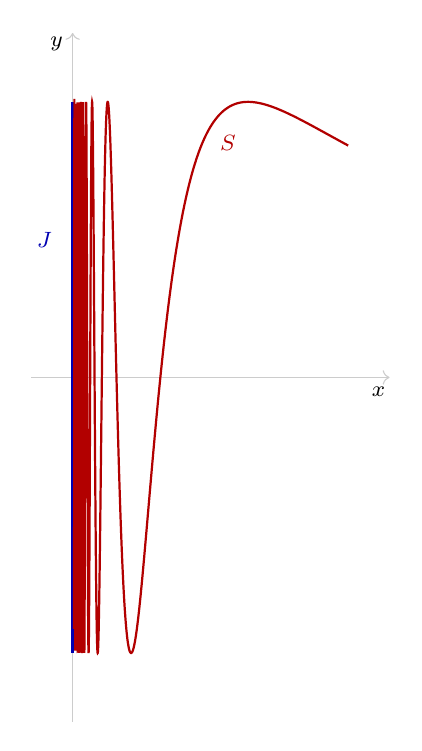
\begin{tikzpicture}[scale=3.5]
  % Axes
  \draw[gray!40, thin, ->] (-0.15,0) -- (1.15,0);
  \draw[gray!40, thin, ->] (0,-1.25) -- (0,1.25);
  % The segment J on the y-axis
  \draw[blue!70!black, very thick] (0,-1) -- (0,1);
  % The curve S = {(x, sin(1/x)) : x in (0,1]}
  \draw[red!70!black, thick, domain=0.005:1, samples=3000, smooth]
    plot (\x, {sin(1/\x r)});
  % Labels
  \node[below right, font=\footnotesize] at (1.05,0) {$x$};
  \node[above left, font=\footnotesize] at (0,1.15) {$y$};
  \node[left, blue!70!black, font=\footnotesize] at (-0.04,0.5) {$J$};
  \node[right, red!70!black, font=\footnotesize] at (0.5,0.85) {$S$};
\end{tikzpicture}
\caption{The topologist's sine curve $T=S\cup J$.  The curve
$S=\{(x,\sin(1/x)):0<x\le 1\}$ oscillates faster and faster
as $x\to 0^+$, and its closure picks up the entire segment $J$.}
\label{fig:topologist-sine-curve}
\end{figure}

\begin{theorem}\label{thm:top-sine-connected-not-path}
The topologist's sine curve $T$ is connected but not path-connected.
\end{theorem}

\begin{proof}
\emph{Connected.}\;
The set $S$ is the image of the continuous map
$(0,1]\to\mathbb{R}^2$, $x\mapsto(x,\sin(1/x))$, and $(0,1]$
is connected (it is an interval), so $S$ is connected.  Since
$S\subseteq T=\overline{S}$, Theorem~\ref{thm:closure-connected}
implies $T$ is connected.

\medskip\noindent
\emph{Not path-connected.}\;
We show there is no path in $T$ from the origin $(0,0)\in J$ to
the point $(1,\sin 1)\in S$.  Suppose for contradiction that
$\gamma\colon[0,1]\to T$ is continuous with $\gamma(0)=(0,0)$
and $\gamma(1)=(1,\sin 1)$.  Write $\gamma(t)=(\gamma_1(t),\gamma_2(t))$.

Define $t_0=\sup\{t\in[0,1]:\gamma_1(t)=0\}$.  Since
$\gamma_1^{-1}(\{0\})$ is closed, $\gamma_1(t_0)=0$.  Moreover
$t_0<1$ because $\gamma_1(1)=1>0$.  For $t>t_0$, we have
$\gamma_1(t)>0$ and $\gamma(t)\in S$, so
$\gamma_2(t)=\sin(1/\gamma_1(t))$.

Since $\gamma_1$ is continuous at $t_0$ with $\gamma_1(t_0)=0$,
the values $\gamma_1(t)\to 0^+$ as $t\to t_0^+$.  Hence
$1/\gamma_1(t)\to+\infty$, and $\sin(1/\gamma_1(t))$ oscillates
between $-1$ and $+1$ without converging.  But $\gamma_2$ is
continuous at $t_0$, so $\gamma_2(t)\to\gamma_2(t_0)$ as
$t\to t_0^+$.  This is a contradiction: $\gamma_2(t)$ cannot
converge and oscillate simultaneously.
\end{proof}

\index{topologist's sine curve|)}

%----------------------------------------------------------
\section{Local Connectedness and Local Path-Connectedness}
\label{sec:local-connectedness}
\index{locally connected|(}
\index{locally path-connected|(}
%----------------------------------------------------------

\begin{definition}\label{def:locally-connected}
A topological space $X$ is \textbf{locally connected}%
\index{locally connected} if for every $x\in X$ and every open
neighborhood $U$ of $x$, there exists a connected open neighborhood
$V$ of $x$ with $V\subseteq U$.

Similarly, $X$ is \textbf{locally path-connected}%
\index{locally path-connected} if every point has arbitrarily small
path-connected open neighborhoods.
\end{definition}

\begin{remark}\label{rem:local-vs-global}
Local (path-)connectedness and global (path-)connectedness are
logically independent.  For instance, the disjoint union
$\mathbb{R}\sqcup\mathbb{R}$ is locally path-connected but not
connected.  The topologist's sine curve is connected but not
locally connected at points of $J$.
\end{remark}

\begin{theorem}\label{thm:connected-lpc-implies-pc}
\index{connectedness!and local path-connectedness}
If $X$ is connected and locally path-connected, then $X$ is
path-connected.
\end{theorem}

\begin{proof}
Fix $x_0\in X$ and let $P$ be the set of all points in $X$ that
can be joined to $x_0$ by a path.  We show $P$ is clopen; since
$X$ is connected and $P\neq\varnothing$ ($x_0\in P$), we conclude
$P=X$.

\emph{$P$ is open.}\; Let $x\in P$.  Since $X$ is locally
path-connected, there exists a path-connected open neighborhood $V$
of $x$.  For every $y\in V$, we can concatenate a path from $x_0$
to $x$ with a path from $x$ to $y$ in $V$, showing $y\in P$.
Hence $V\subseteq P$.

\emph{$P$ is closed.}\; We show $X\setminus P$ is open.  Let
$x\in X\setminus P$ and choose a path-connected open neighborhood
$V$ of $x$.  If some $y\in V$ belonged to $P$, then a path from
$x_0$ to $y$ followed by a path from $y$ to $x$ in $V$ would give
a path from $x_0$ to $x$, contradicting $x\notin P$.  So
$V\subseteq X\setminus P$.
\end{proof}

\index{locally connected|)}
\index{locally path-connected|)}

%----------------------------------------------------------
\section{Totally Disconnected Spaces}
\label{sec:totally-disconnected}
\index{totally disconnected|(}
%----------------------------------------------------------

\begin{definition}\label{def:totally-disconnected}
A topological space $X$ is \textbf{totally disconnected} if the only
connected subsets of $X$ are singletons.  Equivalently, for every
$x\in X$, the connected component of $x$ is $\{x\}$.
\end{definition}

\begin{example}[The rationals]\label{ex:Q-totally-disconnected}
\index{rationals!totally disconnected}
The space $\mathbb{Q}$ (with the subspace topology from $\mathbb{R}$)
is totally disconnected.  Indeed, if $A\subseteq\mathbb{Q}$ contains
two distinct points $p<q$, choose an irrational
$r\in(p,q)$.  Then $A=(A\cap(-\infty,r))\cup(A\cap(r,+\infty))$
is a separation of $A$ in $\mathbb{Q}$, so $A$ is not connected.
\end{example}

\begin{example}[The Cantor set]\label{ex:cantor-totally-disconnected}
\index{Cantor set!totally disconnected}
The Cantor set $\mathcal{C}\subseteq[0,1]$ is totally disconnected.
Each stage of its construction removes an open middle third, and
for any two distinct points $x,y\in\mathcal{C}$ one can find a
removed interval between them, providing a separation of any
subset containing both $x$ and $y$.
\end{example}

\index{totally disconnected|)}

%----------------------------------------------------------
\section{Product of Connected Spaces}
\label{sec:product-connected}
%----------------------------------------------------------

\begin{theorem}\label{thm:product-connected}
\index{connectedness!product}
Let $\{X_i\}_{i\in I}$ be a family of non-empty topological spaces.
The product $\prod_{i\in I}X_i$ (with the product topology) is
connected if and only if each $X_i$ is connected.
\end{theorem}

\begin{proof}
\emph{``Only if.''}\; Each projection
$\pi_j\colon\prod_{i\in I}X_i\to X_j$ is continuous and surjective,
so by Theorem~\ref{thm:continuous-image-connected}, $X_j$ is connected.

\medskip\noindent
\emph{``If.''}\;  We prove the result in two steps.

\emph{Step 1: Finite products.}\;
It suffices to prove $X\times Y$ is connected whenever $X$ and $Y$
are connected, and then iterate.  Fix a point $(a,b)\in X\times Y$.
For each $x\in X$, the ``horizontal slice''
$\{x\}\times Y \cong Y$ is connected, and the ``vertical slice''
$X\times\{b\}\cong X$ is connected.  The set
\[
   T_x = (X\times\{b\})\cup(\{x\}\times Y)
\]
is the union of two connected sets sharing the point $(x,b)$, so
$T_x$ is connected by Theorem~\ref{thm:union-connected-common-point}.
Moreover, each $T_x$ contains $(a,b)$ (because $(a,b)\in X\times\{b\}
\subseteq T_x$), so
\[
   X\times Y = \bigcup_{x\in X}T_x
\]
is connected by Theorem~\ref{thm:union-connected-common-point} again.

\emph{Step 2: Arbitrary products.}\;
Fix a point $\mathbf{a}=(a_i)_{i\in I}\in\prod X_i$.  For each
finite subset $F\subseteq I$, let
\[
   Y_F = \Bigl\{\,\mathbf{x}\in\prod X_i : x_i=a_i
                  \text{ for all }i\notin F\Bigr\}.
\]
Then $Y_F\cong\prod_{i\in F}X_i$, which is connected by Step~1.
Moreover $\mathbf{a}\in Y_F$ for all $F$, so
$Z=\bigcup_{F\subseteq I,\,|F|<\infty}Y_F$ is connected.  We claim
$Z$ is dense in $\prod X_i$.  A basic open set in the product topology
restricts only finitely many coordinates, say those in a finite set $F$,
and agrees with $\prod X_i$ on the remaining coordinates.  Hence any
basic open set meeting $\prod X_i$ also meets $Y_F\subseteq Z$.
Therefore $\overline{Z}=\prod X_i$, and by
Theorem~\ref{thm:closure-connected}, $\prod X_i$ is connected.
\end{proof}

%----------------------------------------------------------
\section{Illustrations}
%----------------------------------------------------------

\begin{figure}[ht]
\centering
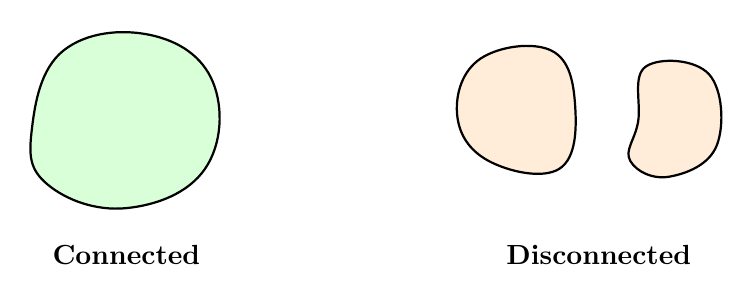
\begin{tikzpicture}[scale=1.0]
  % Connected set
  \begin{scope}[shift={(-3.5,0)}]
    \draw[thick, fill=green!15] plot[smooth cycle, tension=0.7]
      coordinates{(-1.2,0) (-0.8,1) (0.3,1.2) (1.1,0.6) (1,-0.5) (0,-1) (-1,-0.7)};
    \node[font=\bfseries] at (0,-1.6) {Connected};
  \end{scope}
  % Disconnected set
  \begin{scope}[shift={(2.5,0)}]
    \draw[thick, fill=orange!15] plot[smooth cycle, tension=0.7]
      coordinates{(-1.8,0.2) (-1.5,0.9) (-0.6,1) (-0.3,0.3) (-0.5,-0.5) (-1.4,-0.4)};
    \draw[thick, fill=orange!15] plot[smooth cycle, tension=0.7]
      coordinates{(0.5,0.1) (0.6,0.8) (1.4,0.7) (1.5,-0.2) (0.9,-0.6) (0.4,-0.4)};
    \node[font=\bfseries] at (0,-1.6) {Disconnected};
  \end{scope}
\end{tikzpicture}
\caption{A connected set (left) versus a disconnected set consisting of two components (right).}
\label{fig:connected-vs-disconnected}
\end{figure}

\begin{figure}[ht]
\centering
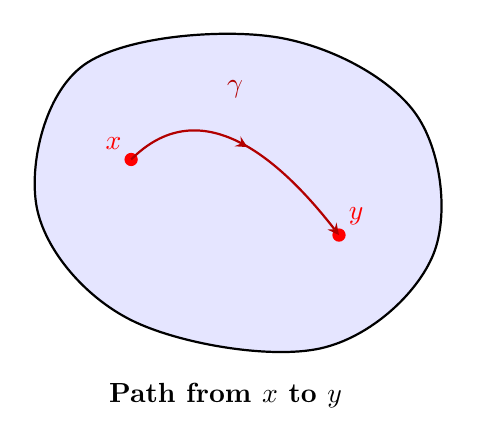
\begin{tikzpicture}[scale=1.2]
  % Points and path
  \draw[thick, fill=blue!10] plot[smooth cycle, tension=0.6]
    coordinates{(-2,0) (-1.5,1.5) (0.5,1.8) (2,1) (2.2,-0.5) (1,-1.5) (-1,-1.2)};
  \fill[red] (-1,0.5) circle (2pt) node[above left]{$x$};
  \fill[red] (1.2,-0.3) circle (2pt) node[above right]{$y$};
  \draw[thick, red!70!black, ->, >=stealth,
        postaction={decorate, decoration={markings,
        mark=at position 0.5 with {\arrow{>}}}}]
    (-1,0.5) .. controls (-0.3,1.2) and (0.5,0.6) .. (1.2,-0.3);
  \node[red!70!black, above] at (0.1,1.05) {$\gamma$};
  \node[font=\bfseries] at (0,-2.0) {Path from $x$ to $y$};
\end{tikzpicture}
\caption{A path $\gamma\colon[0,1]\to X$ joining $x$ to $y$ in a
path-connected space.}
\label{fig:path-illustration}
\end{figure}

%----------------------------------------------------------
\section{Worked Examples}
\label{sec:connected-examples}
%----------------------------------------------------------

\begin{example}[Intervals are connected]\label{ex:intervals-connected}
\index{interval!connected}
Every interval $I\subseteq\mathbb{R}$ is connected.  Suppose
$(U,V)$ is a separation of $I$ and pick $a\in U$, $b\in V$ with
$a<b$.  Let $c=\sup(U\cap[a,b])$.  Since $U$ is closed in $I$
(it is the complement of the open set $V$), we have $c\in U$.
Since $U$ is also open in $I$, there is an $\varepsilon>0$ with
$(c-\varepsilon,c+\varepsilon)\cap I\subseteq U$.  Because $c<b$
(as $b\in V$ and $U\cap V=\varnothing$), there exist points of
$U\cap[a,b]$ greater than $c$, contradicting the definition of $c$.
Hence no separation exists.
\end{example}

\begin{example}[$\mathbb{R}^n$ is connected]\label{ex:Rn-connected}
\index{Euclidean space!connected}
For any two points $x,y\in\mathbb{R}^n$, the map
$\gamma(t)=(1-t)x+ty$ is a path from $x$ to $y$.  Hence
$\mathbb{R}^n$ is path-connected, therefore connected.
\end{example}

\begin{example}[$S^n$ is connected for $n\ge 1$]
\label{ex:sphere-connected}
\index{sphere!connected}
The sphere $S^n=\{x\in\mathbb{R}^{n+1}:\|x\|=1\}$ for $n\ge 1$ is
path-connected: given $p,q\in S^n$, if $p\neq -q$ the great-circle
arc gives a path; if $p=-q$ we pass through any third point.  Hence
$S^n$ is connected.  (For $n=0$, $S^0=\{-1,1\}$ is disconnected.)
\end{example}

\begin{example}[$\mathrm{GL}_n(\mathbb{R})$ is disconnected]
\label{ex:GLn-disconnected}
\index{general linear group!disconnected}
The determinant $\det\colon\mathrm{GL}_n(\mathbb{R})\to
\mathbb{R}\setminus\{0\}$ is continuous.  The image
$\mathbb{R}\setminus\{0\}=(-\infty,0)\cup(0,\infty)$ is disconnected,
and the preimages $\mathrm{GL}_n^+(\mathbb{R})$ and
$\mathrm{GL}_n^-(\mathbb{R})$ are both non-empty, open, and disjoint.
Hence $\mathrm{GL}_n(\mathbb{R})$ is disconnected (it has exactly
two connected components).
\end{example}

%----------------------------------------------------------
\section{Exercises}
\label{sec:connected-exercises}
%----------------------------------------------------------

\begin{exercise}[$\bigstar$]\label{exo:connected-R-minus-point}
Show that $\mathbb{R}\setminus\{0\}$ is disconnected, and determine
its connected components.
\end{exercise}

\begin{exercise}[$\bigstar$]\label{exo:connected-subsets-R}
Prove that the connected subsets of $\mathbb{R}$ are precisely the
intervals (including the empty set, singletons, rays, and
$\mathbb{R}$ itself).
\end{exercise}

\begin{exercise}[$\bigstar$]\label{exo:fixed-point-interval}
Use the Intermediate Value Theorem to prove that every continuous
map $f\colon[0,1]\to[0,1]$ has a fixed point.
\end{exercise}

\begin{exercise}[$\bigstar\bigstar$]\label{exo:connected-complement-Rn}
Show that $\mathbb{R}^n\setminus\{p\}$ is connected for $n\ge 2$
and any $p\in\mathbb{R}^n$.  \textit{Hint:} show it is
path-connected.
\end{exercise}

\begin{exercise}[$\bigstar\bigstar$]\label{exo:closure-interior-connected}
Let $A\subseteq\mathbb{R}^n$ be open and connected.  Is
$\overline{A}$ necessarily connected?  Is the interior of a closed
connected set necessarily connected?  Justify or give counterexamples.
\end{exercise}

\begin{exercise}[$\bigstar\bigstar$]\label{exo:connected-quotient}
Let $X$ be a connected space and $\sim$ an equivalence relation
on $X$.  Show that the quotient space $X/{\sim}$ is connected.
\end{exercise}

\begin{exercise}[$\bigstar\bigstar$]\label{exo:components-totally-disconnected}
Let $X$ be a topological space and let $X/{\sim}$ be the quotient
space obtained by collapsing each connected component to a point.
Show that $X/{\sim}$ is totally disconnected.
\end{exercise}

\begin{exercise}[$\bigstar\bigstar\bigstar$]\label{exo:polish-circle}
\index{Warsaw circle}
The \emph{Warsaw circle} (or \emph{Polish circle}) is obtained by
connecting the endpoints $(0,-1)$ and $(1,\sin 1)$ of the topologist's
sine curve $T$ by an arc in $\mathbb{R}^2$ that does not otherwise
intersect $T$.  Show that the Warsaw circle is connected but not
path-connected.
\end{exercise}

\begin{exercise}[$\bigstar\bigstar\bigstar$]\label{exo:cantor-characterization}
Prove that the Cantor set $\mathcal{C}$ is totally disconnected,
compact, metrizable, and has no isolated points.  (In fact, up to
homeomorphism, $\mathcal{C}$ is the unique such space.)
\end{exercise}

%----------------------------------------------------------
\section*{Chapter Summary}
%----------------------------------------------------------

\begin{itemize}
\item A space is \textbf{connected} if it has no separation.
      Equivalently, its only clopen subsets are $\varnothing$ and
      the whole space.
\item Continuous images of connected spaces are connected, yielding
      the Intermediate Value Theorem.
\item If $A$ is connected and $A\subseteq B\subseteq\overline{A}$,
      then $B$ is connected.  Unions of connected sets sharing a
      common point are connected.
\item \textbf{Path-connected} $\Longrightarrow$ \textbf{connected},
      but the converse fails (topologist's sine curve).
\item Connected $+$ locally path-connected $\Longrightarrow$
      path-connected.
\item \textbf{Totally disconnected} means every connected component
      is a singleton (e.g.\ $\mathbb{Q}$, the Cantor set).
\item Arbitrary products of connected spaces are connected
      (product topology).
\end{itemize}

\index{connectedness|)}
\index{path-connectedness|)}


%%%%%%%%%%%%%%%%%%%%%%%%%%%%%%%%%%%%%%%%%%%%%%%%%%%%%%%%%%%%%
\chapter{Product Spaces and Quotient Topology}\label{ch:product-quotient}
%%%%%%%%%%%%%%%%%%%%%%%%%%%%%%%%%%%%%%%%%%%%%%%%%%%%%%%%%%%%%

\index{product topology|(}
\index{quotient topology|(}

Topology provides systematic machinery for building new spaces
from old ones.  Two of the most fundamental constructions are the
\emph{product}, which assembles spaces ``side by side,'' and the
\emph{quotient}, which identifies points according to an equivalence
relation, effectively ``gluing'' parts of a space together.  These
constructions underpin nearly every geometric object studied in
algebraic topology and differential geometry: tori, projective spaces,
and fiber bundles all arise through products and quotients.

%----------------------------------------------------------
\section{Finite Products}\label{sec:finite-products}
\index{product topology!finite}
%----------------------------------------------------------

\begin{definition}[Product topology --- finite case]
\label{def:product-topology-finite}
Let $X_1,\dots,X_n$ be topological spaces.  The \textbf{product
topology} on $X_1\times\cdots\times X_n$ is the topology generated
by the basis
\[
   \mathcal{B} = \bigl\{\,U_1\times\cdots\times U_n :
     U_i\text{ open in }X_i,\ i=1,\dots,n\bigr\}.
\]
The projections $\pi_j\colon X_1\times\cdots\times X_n\to X_j$
are defined by $\pi_j(x_1,\dots,x_n)=x_j$.
\end{definition}

\begin{remark}\label{rem:finite-product-basis}
In the finite case, the set $\mathcal{B}$ is itself a basis (it is
closed under finite intersections), and the product topology coincides
with the topology generated by all sets of the form
$\pi_j^{-1}(U_j)=X_1\times\cdots\times U_j\times\cdots\times X_n$.
\end{remark}

%----------------------------------------------------------
\section{Infinite Products: Product vs.\ Box Topology}
\label{sec:infinite-products}
\index{product topology!infinite}
\index{box topology|(}
%----------------------------------------------------------

\begin{definition}\label{def:product-box-topology}
Let $\{X_i\}_{i\in I}$ be a family of topological spaces and let
$X=\prod_{i\in I}X_i$.
\begin{enumerate}
\item The \textbf{box topology}\index{box topology} on $X$ is the
      topology generated by the basis
      \[
         \mathcal{B}_{\mathrm{box}} = \Bigl\{\,\prod_{i\in I}U_i :
            U_i\text{ open in }X_i\text{ for all }i\in I\Bigr\}.
      \]
\item The \textbf{product topology} on $X$ is the topology generated
      by the subbasis
      \[
         \mathcal{S} = \bigl\{\,\pi_i^{-1}(U_i) : i\in I,\;
            U_i\text{ open in }X_i\bigr\}.
      \]
      A basis for the product topology consists of sets of the form
      $\prod_{i\in I}U_i$ where $U_i=X_i$ for all but finitely
      many $i$.
\end{enumerate}
\end{definition}

\begin{remark}\label{rem:box-vs-product}
For finite index sets, the two topologies coincide.  For infinite
index sets, the product topology is strictly coarser than the box
topology.  The product topology is the ``correct'' topology for
most purposes: it makes the product a categorical product (see
Theorem~\ref{thm:product-universal} and
Section~\ref{sec:universal-product}).
\end{remark}

%----------------------------------------------------------
\section{Universal Property and Projections}
\label{sec:universal-product}
%----------------------------------------------------------

\begin{theorem}[Coarsest topology for projections]
\label{thm:product-coarsest}
\index{product topology!coarsest for projections}
The product topology on $X=\prod_{i\in I}X_i$ is the coarsest
topology on $X$ such that every projection
$\pi_j\colon X\to X_j$ is continuous.
\end{theorem}

\begin{proof}
In the product topology, each $\pi_j$ is continuous because
$\pi_j^{-1}(U_j)\in\mathcal{S}$ for every open $U_j\subseteq X_j$.

Conversely, let $\tau$ be any topology on $X$ making all projections
continuous.  Then $\pi_j^{-1}(U_j)\in\tau$ for every $j\in I$ and
every open $U_j\subseteq X_j$.  Since the product topology is
generated by exactly these sets, we have $\tau_{\mathrm{prod}}\subseteq\tau$.
\end{proof}

\begin{theorem}[Universal property of the product]
\label{thm:product-universal}
\index{product topology!universal property}
Let $X=\prod_{i\in I}X_i$ carry the product topology.  A map
$f\colon Y\to X$ is continuous if and only if $\pi_i\circ f$ is
continuous for every $i\in I$.
\end{theorem}

\begin{proof}
\emph{``Only if.''}\; If $f$ is continuous, then $\pi_i\circ f$ is
a composition of continuous maps, hence continuous.

\emph{``If.''}\; Suppose $\pi_i\circ f$ is continuous for all $i$.
For each subbasis element $\pi_i^{-1}(U_i)$,
\[
   f^{-1}\bigl(\pi_i^{-1}(U_i)\bigr) = (\pi_i\circ f)^{-1}(U_i)
\]
is open in $Y$.  Since the product topology is generated by the
subbasis $\mathcal{S}=\{\pi_i^{-1}(U_i)\}$, and the preimage of
any finite intersection or arbitrary union of such sets is likewise
open, $f$ is continuous.
\end{proof}

\begin{proposition}[Projections are open maps]
\label{prop:projections-open}
\index{projection!open map}
Each projection $\pi_j\colon\prod_{i\in I}X_i\to X_j$ is an open map.
\end{proposition}

\begin{proof}
It suffices to show that $\pi_j$ maps basis elements to open sets.
A basic open set in the product topology is
$B=\prod_{i\in I}U_i$ with $U_i=X_i$ for all but finitely many $i$
and $U_i$ open in $X_i$ for all $i$.  Then
$\pi_j(B)=U_j$, which is open in $X_j$.
\end{proof}

\begin{remark}\label{rem:projections-not-closed}
Projections are not necessarily closed maps.  For example, the set
$C=\{(x,y)\in\mathbb{R}^2 : xy=1\}$ is closed in $\mathbb{R}^2$,
but $\pi_1(C)=\mathbb{R}\setminus\{0\}$ is not closed
in $\mathbb{R}$.
\end{remark}

%----------------------------------------------------------
\section{The Tube Lemma}\label{sec:tube-lemma}
\index{tube lemma}
%----------------------------------------------------------

\begin{lemma}[Tube Lemma]\label{lem:tube}
Let $X$ and $Y$ be topological spaces with $Y$ compact.  Let
$x_0\in X$ and let $N$ be an open subset of $X\times Y$ containing
the ``slice'' $\{x_0\}\times Y$.  Then there exists an open set
$W\subseteq X$ containing $x_0$ such that $\{x_0\}\times Y
\subseteq W\times Y\subseteq N$.
\end{lemma}

\begin{proof}
For each $y\in Y$, the point $(x_0,y)\in N$, so there exist open
sets $U_y\subseteq X$ and $V_y\subseteq Y$ with
$(x_0,y)\in U_y\times V_y\subseteq N$.  The collection
$\{V_y\}_{y\in Y}$ is an open cover of $Y$.  Since $Y$ is compact,
there is a finite subcover $V_{y_1},\dots,V_{y_m}$.  Set
\[
   W = U_{y_1}\cap\cdots\cap U_{y_m}.
\]
Then $W$ is open, $x_0\in W$, and for any $(w,y)\in W\times Y$,
we have $y\in V_{y_k}$ for some $k$, so
$(w,y)\in U_{y_k}\times V_{y_k}\subseteq N$.  Hence
$W\times Y\subseteq N$.
\end{proof}

%----------------------------------------------------------
\section{Products and Separation}
\label{sec:product-separation}
%----------------------------------------------------------

\begin{theorem}\label{thm:product-hausdorff}
\index{Hausdorff!product}
The product $\prod_{i\in I}X_i$ (with the product topology) is
Hausdorff if and only if each $X_i$ is Hausdorff.
\end{theorem}

\begin{proof}
\emph{``Only if.''}\; Each $X_j$ is the continuous image of the
projection, and a subspace of a Hausdorff space is Hausdorff.
More precisely, if $(x_i)$ and $(y_i)$ differ in coordinate $j$
with $x_j\neq y_j$, and we can separate them in the product, then
projecting gives a separation in $X_j$.

\emph{``If.''}\; Let $\mathbf{x}=(x_i)$ and $\mathbf{y}=(y_i)$
be distinct points in $\prod X_i$.  There exists $j\in I$ with
$x_j\neq y_j$.  Since $X_j$ is Hausdorff, choose disjoint open
sets $U_j,V_j\subseteq X_j$ with $x_j\in U_j$ and $y_j\in V_j$.
Then $\pi_j^{-1}(U_j)$ and $\pi_j^{-1}(V_j)$ are disjoint open
sets in $\prod X_i$ separating $\mathbf{x}$ and $\mathbf{y}$.
\end{proof}

%----------------------------------------------------------
\section{Quotient Topology}\label{sec:quotient-topology}
\index{quotient topology}
\index{quotient map}
%----------------------------------------------------------

\begin{definition}[Quotient map and quotient topology]
\label{def:quotient-map}
Let $X$ be a topological space, $Y$ a set, and $q\colon X\to Y$
a surjection.  The \textbf{quotient topology} on $Y$ (induced
by $q$) is
\[
   \tau_Y = \bigl\{\,V\subseteq Y : q^{-1}(V)\text{ is open in }X\bigr\}.
\]
With this topology, $q$ is called a \textbf{quotient map}.

If $\sim$ is an equivalence relation on $X$, the \textbf{quotient
space} $X/{\sim}$ is the set of equivalence classes equipped with
the quotient topology induced by the canonical projection
$q\colon X\to X/{\sim}$, $q(x)=[x]$.
\end{definition}

\begin{definition}[Saturated set]\label{def:saturated}
\index{saturated set}
A subset $A\subseteq X$ is \textbf{saturated} with respect to
a surjection $q\colon X\to Y$ if $A=q^{-1}(q(A))$; that is,
$A$ is a union of fibers $q^{-1}(\{y\})$.
\end{definition}

\begin{remark}\label{rem:saturated-characterization}
A subset $V\subseteq Y$ is open in the quotient topology if and
only if $q^{-1}(V)$ is a saturated open subset of $X$.  Thus the
open sets of $X/{\sim}$ correspond bijectively to the saturated
open subsets of $X$.
\end{remark}

\begin{theorem}[Universal property of the quotient]
\label{thm:quotient-universal}
\index{quotient topology!universal property}
Let $q\colon X\to Y$ be a quotient map and $f\colon X\to Z$ a
continuous map that is constant on the fibers of $q$ (i.e.,
$q(x)=q(x')$ implies $f(x)=f(x')$).  Then there exists a unique
continuous map $\bar{f}\colon Y\to Z$ such that $f=\bar{f}\circ q$.
\[
\begin{tikzcd}
X \arrow[r, "q"] \arrow[dr, "f"'] & Y \arrow[d, dashed, "\bar{f}"] \\
& Z
\end{tikzcd}
\]
\end{theorem}

\begin{proof}
\emph{Existence and uniqueness.}\;
Define $\bar{f}(y)=f(x)$ for any $x\in q^{-1}(\{y\})$.  This is
well-defined because $f$ is constant on fibers of $q$.  By
construction $f=\bar{f}\circ q$, and uniqueness is immediate since
$q$ is surjective.

\emph{Continuity.}\;
Let $W\subseteq Z$ be open.  Then
$q^{-1}(\bar{f}^{-1}(W))=(\bar{f}\circ q)^{-1}(W)=f^{-1}(W)$,
which is open in $X$ because $f$ is continuous.  By definition
of the quotient topology, $\bar{f}^{-1}(W)$ is open in $Y$.
\end{proof}

\begin{theorem}[Continuity via quotient maps]
\label{thm:continuity-via-quotient}
Let $q\colon X\to Y$ be a quotient map.  A map $g\colon Y\to Z$
is continuous if and only if $g\circ q\colon X\to Z$ is continuous.
\end{theorem}

\begin{proof}
\emph{``Only if.''}\; A composition of continuous maps is continuous.

\emph{``If.''}\; Let $W\subseteq Z$ be open.  Then
$q^{-1}(g^{-1}(W))=(g\circ q)^{-1}(W)$ is open in $X$.  By definition
of the quotient topology, $g^{-1}(W)$ is open in $Y$.
\end{proof}

%----------------------------------------------------------
\section{Quotient Examples with Identification Diagrams}
\label{sec:quotient-examples}
%----------------------------------------------------------

% ---- Circle ----
\begin{example}[The circle $S^1$]\label{ex:circle-quotient}
\index{circle!as quotient}
Define an equivalence relation on $[0,1]$ by $0\sim 1$ (and $x\sim x$
for all $x$).  The quotient $[0,1]/(0\sim 1)$ is homeomorphic
to $S^1$.

The quotient map is $q\colon[0,1]\to S^1$, $q(t)=e^{2\pi it}$.
This map is continuous, surjective, and since $[0,1]$ is compact
and $S^1$ is Hausdorff, $q$ is a quotient map.  It identifies only
$0$ and $1$, so it descends to a continuous bijection
$[0,1]/(0\sim 1)\to S^1$, which is a homeomorphism (continuous
bijection from a compact space to a Hausdorff space).
\end{example}

\begin{figure}[ht]
\centering
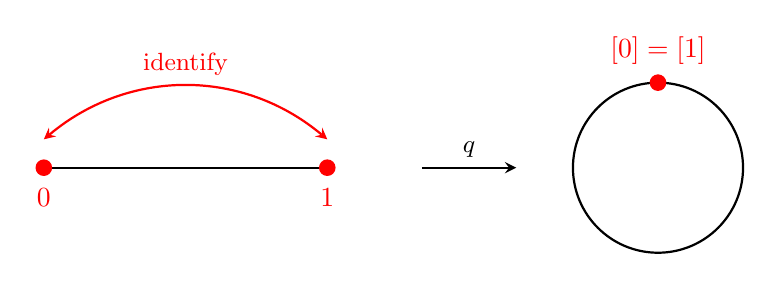
\begin{tikzpicture}[scale=1.2]
  % Interval [0,1] with identification
  \draw[thick] (0,0) -- (3,0);
  \fill[red] (0,0) circle (2.5pt) node[below=4pt]{$0$};
  \fill[red] (3,0) circle (2.5pt) node[below=4pt]{$1$};
  \draw[thick, red, <->, >=stealth] (0,0.3) to[bend left=40]
    node[above, font=\small]{identify} (3,0.3);
  % Arrow
  \draw[->, thick, >=stealth] (4,0) -- (5,0)
    node[midway, above, font=\small]{$q$};
  % Circle
  \draw[thick] (6.5,0) circle (0.9);
  \fill[red] (6.5,0.9) circle (2.5pt) node[above=3pt]{$[0]=[1]$};
\end{tikzpicture}
\caption{The circle $S^1$ as the quotient $[0,1]/(0\sim 1)$.}
\label{fig:circle-quotient}
\end{figure}

% ---- Torus ----
\begin{example}[The torus $T^2$]\label{ex:torus-quotient}
\index{torus!as quotient}
Define an equivalence relation on $[0,1]^2$ by identifying opposite
edges:
\[
   (0,t)\sim(1,t)\quad\text{and}\quad(s,0)\sim(s,1)
   \qquad\text{for all }s,t\in[0,1].
\]
The quotient $[0,1]^2/{\sim}$ is homeomorphic to the torus
$T^2=S^1\times S^1$.  Indeed, the map
$q(s,t)=(e^{2\pi is},\,e^{2\pi it})$ is a quotient map realizing
this identification.
\end{example}

\begin{figure}[ht]
\centering
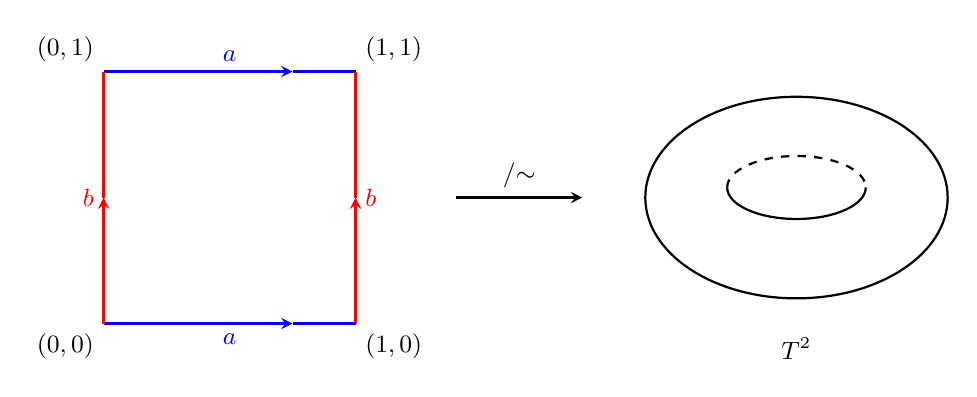
\begin{tikzpicture}[scale=1.6]
  % Square with identifications
  \draw[thick, blue, ->, >=stealth] (0,0) -- (1.5,0);
  \draw[thick, blue, ->, >=stealth] (0,2) -- (1.5,2);
  \draw[thick, red, ->, >=stealth] (0,0) -- (0,1);
  \draw[thick, red, ->, >=stealth] (2,0) -- (2,1);
  \draw[thick, blue] (1.5,0) -- (2,0);
  \draw[thick, blue] (1.5,2) -- (2,2);
  \draw[thick, red] (0,1) -- (0,2);
  \draw[thick, red] (2,1) -- (2,2);
  \node[below left, font=\small] at (0,0) {$(0,0)$};
  \node[below right, font=\small] at (2,0) {$(1,0)$};
  \node[above left, font=\small] at (0,2) {$(0,1)$};
  \node[above right, font=\small] at (2,2) {$(1,1)$};
  % Labels for edge identification
  \node[below, blue, font=\small\bfseries] at (1,0) {$a$};
  \node[above, blue, font=\small\bfseries] at (1,2) {$a$};
  \node[left, red, font=\small\bfseries] at (0,1) {$b$};
  \node[right, red, font=\small\bfseries] at (2,1) {$b$};
  % Arrow
  \draw[->, thick, >=stealth] (2.8,1) -- (3.8,1)
    node[midway, above, font=\small]{$/{\sim}$};
  % Torus (schematic)
  \begin{scope}[shift={(5.5,1)}]
    \draw[thick] (0,0) ellipse (1.2 and 0.8);
    \draw[thick] (-0.55,0.08) arc (180:360:0.55 and 0.25);
    \draw[thick, dashed] (-0.55,0.08) arc (180:0:0.55 and 0.25);
    \node[font=\small\bfseries] at (0,-1.2) {$T^2$};
  \end{scope}
\end{tikzpicture}
\caption{The torus $T^2$ obtained by identifying opposite edges of
the unit square with matching orientations.  Edges labeled $a$ are
identified, as are edges labeled $b$.}
\label{fig:torus-quotient}
\end{figure}

% ---- Mobius band ----
\begin{example}[The M\"obius band]\label{ex:mobius-quotient}
\index{Mobius band@M\"obius band}
On $[0,1]^2$, identify $(0,t)\sim(1,1-t)$ for all $t\in[0,1]$.
This reverses the orientation of one pair of opposite edges, yielding
the M\"obius band\index{Mobius band@M\"obius band!as quotient}.
\end{example}

\begin{figure}[ht]
\centering
\begin{tikzpicture}[scale=1.6]
  % Square with identifications
  \draw[thick, gray] (0,0) -- (2,0);
  \draw[thick, gray] (0,2) -- (2,2);
  \draw[thick, red, ->, >=stealth] (0,0) -- (0,1);
  \draw[thick, red] (0,1) -- (0,2);
  \draw[thick, blue, <-, >=stealth] (2,1) -- (2,2);
  \draw[thick, blue] (2,0) -- (2,1);
  % Labels
  \node[left, red, font=\small\bfseries] at (0,1) {$a$};
  \node[right, blue, font=\small\bfseries] at (2,1) {$a$};
  % Note the opposing arrows
  \node[below, font=\small] at (1,0) {\textit{free}};
  \node[above, font=\small] at (1,2) {\textit{free}};
\end{tikzpicture}
\caption{The M\"obius band: the edges labeled $a$ are identified
with reversed orientations (note the opposing arrows).}
\label{fig:mobius-quotient}
\end{figure}

% ---- Klein bottle ----
\begin{example}[The Klein bottle]\label{ex:klein-quotient}
\index{Klein bottle}
On $[0,1]^2$, identify $(0,t)\sim(1,1-t)$ and $(s,0)\sim(s,1)$.
The first identification reverses one pair of edges (as for the
M\"obius band), and the second identifies the other pair with
matching orientations.  The resulting quotient is the Klein bottle,
which cannot be embedded in $\mathbb{R}^3$ without self-intersection.
\end{example}

\begin{figure}[ht]
\centering
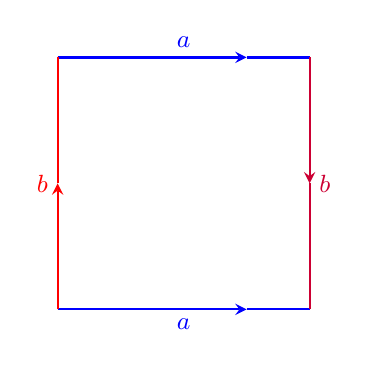
\begin{tikzpicture}[scale=1.6]
  \draw[thick, blue, ->, >=stealth] (0,0) -- (1.5,0);
  \draw[thick, blue, ->, >=stealth] (0,2) -- (1.5,2);
  \draw[thick, blue] (1.5,0) -- (2,0);
  \draw[thick, blue] (1.5,2) -- (2,2);
  \draw[thick, red, ->, >=stealth] (0,0) -- (0,1);
  \draw[thick, red] (0,1) -- (0,2);
  \draw[thick, red!80!blue, <-, >=stealth] (2,1) -- (2,2);
  \draw[thick, red!80!blue] (2,0) -- (2,1);
  \node[below, blue, font=\small\bfseries] at (1,0) {$a$};
  \node[above, blue, font=\small\bfseries] at (1,2) {$a$};
  \node[left, red, font=\small\bfseries] at (0,1) {$b$};
  \node[right, red!80!blue, font=\small\bfseries] at (2,1) {$b$};
\end{tikzpicture}
\caption{The Klein bottle: edges $a$ are identified with the same
orientation, but edges $b$ are identified with reversed orientation.}
\label{fig:klein-quotient}
\end{figure}

% ---- Real projective plane ----
\begin{example}[The real projective plane $\mathbb{R}P^2$]
\label{ex:RP2-quotient}
\index{real projective plane}
There are two common descriptions.
\begin{enumerate}
\item \emph{As a quotient of $S^2$.}\;
      On the $2$-sphere $S^2$, identify antipodal points:
      $x\sim -x$.  The quotient $S^2/{\sim}$ is $\mathbb{R}P^2$.
\item \emph{As a quotient of a square.}\;
      On $[0,1]^2$, identify $(0,t)\sim(1,1-t)$ and
      $(s,0)\sim(1-s,1)$.  Both pairs of opposite edges are
      identified with reversed orientations.
\end{enumerate}
The resulting space is non-orientable and cannot be embedded
in $\mathbb{R}^3$.
\end{example}

\begin{figure}[ht]
\centering
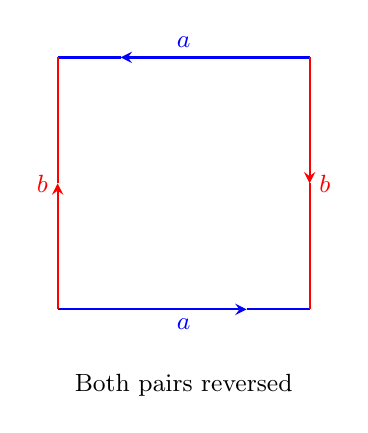
\begin{tikzpicture}[scale=1.6]
  % Square with all reversed identifications
  \draw[thick, blue, ->, >=stealth] (0,0) -- (1.5,0);
  \draw[thick, blue] (1.5,0) -- (2,0);
  \draw[thick, blue, <-, >=stealth] (0.5,2) -- (2,2);
  \draw[thick, blue] (0,2) -- (0.5,2);
  \draw[thick, red, ->, >=stealth] (0,0) -- (0,1);
  \draw[thick, red] (0,1) -- (0,2);
  \draw[thick, red, <-, >=stealth] (2,1) -- (2,2);
  \draw[thick, red] (2,0) -- (2,1);
  \node[below, blue, font=\small\bfseries] at (1,0) {$a$};
  \node[above, blue, font=\small\bfseries] at (1,2) {$a$};
  \node[left, red, font=\small\bfseries] at (0,1) {$b$};
  \node[right, red, font=\small\bfseries] at (2,1) {$b$};
  % Note
  \node[font=\small] at (1,-0.6) {Both pairs reversed};
\end{tikzpicture}
\caption{The real projective plane $\mathbb{R}P^2$: both pairs
of opposite edges are identified with reversed orientations.}
\label{fig:RP2-quotient}
\end{figure}

%----------------------------------------------------------
\section{Disjoint Union (Coproduct) Topology}
\label{sec:disjoint-union}
\index{disjoint union topology}
\index{coproduct topology}
%----------------------------------------------------------

\begin{definition}\label{def:disjoint-union}
Let $\{X_i\}_{i\in I}$ be a family of topological spaces.  The
\textbf{disjoint union} (or \textbf{coproduct}) is the set
\[
   \coprod_{i\in I}X_i = \bigcup_{i\in I}\{i\}\times X_i,
\]
equipped with the topology in which $U\subseteq\coprod X_i$ is open
if and only if $U\cap(\{i\}\times X_i)$ is open in $X_i$ for every
$i\in I$.  Equivalently, it is the finest topology making each
canonical injection $\iota_j\colon X_j\to\coprod X_i$ continuous.
\end{definition}

\begin{proposition}\label{prop:coproduct-universal}
\index{coproduct topology!universal property}
A map $f\colon\coprod_{i\in I}X_i\to Y$ is continuous if and only
if $f\circ\iota_i\colon X_i\to Y$ is continuous for every $i\in I$.
\end{proposition}

\begin{proof}
\emph{``Only if.''}\; Compositions of continuous maps are continuous.

\emph{``If.''}\;
Let $V\subseteq Y$ be open.  Then
$f^{-1}(V)\cap(\{i\}\times X_i) = \iota_i^{-1}(f^{-1}(V))
= (f\circ\iota_i)^{-1}(V)$,
which is open in $X_i$ by hypothesis.  By definition of the
disjoint union topology, $f^{-1}(V)$ is open.
\end{proof}

%----------------------------------------------------------
\section{Box Topology Pathologies}\label{sec:box-pathologies}
\index{box topology!pathologies}
%----------------------------------------------------------

The box topology, while seemingly natural, has severe pathological
properties for infinite products that make it poorly suited to
general theory.

\begin{theorem}\label{thm:box-pathologies}
Let $\mathbb{R}^\omega=\prod_{n=1}^{\infty}\mathbb{R}$ equipped
with the box topology.  Then:
\begin{enumerate}
\item $\mathbb{R}^\omega$ with the box topology is \textbf{not
      connected}.\label{item:box-not-connected}
\item $\mathbb{R}^\omega$ with the box topology is \textbf{not
      second countable}.\label{item:box-not-2nd-countable}
\item $\mathbb{R}^\omega$ with the box topology is \textbf{not
      metrizable}.\label{item:box-not-metrizable}
\end{enumerate}
\end{theorem}

\begin{proof}
(\ref{item:box-not-connected})\;
Let $B$ denote the set of bounded sequences and $U$ the set of
unbounded sequences.  We claim both are open in the box topology.
For any bounded sequence $(x_n)$ with $|x_n|\le M$ for all $n$,
the box-open set $\prod_{n=1}^{\infty}(-M-1,M+1)$ is a neighborhood
contained in $B$.  For any unbounded sequence $(x_n)$, choose a
subsequence $|x_{n_k}|\to\infty$ and for each $n_k$ take an interval
$(x_{n_k}-1,x_{n_k}+1)$, and for other coordinates take all
of $\mathbb{R}$; the resulting box-open set lies within $U$.
Since $B$ and $U$ are non-empty, open, disjoint, and cover
$\mathbb{R}^\omega$, it is disconnected.

\medskip\noindent
(\ref{item:box-not-2nd-countable})\;
For each function $f\colon\mathbb{N}\to\mathbb{R}$, the box-open set
$\prod_{n=1}^{\infty}(f(n)-1,\,f(n)+1)$ contains the point
$(f(n))_{n\ge 1}$ but does not contain any point $(g(n))$ with
$|g(k)-f(k)|\ge 1$ for some $k$.  These form an uncountable collection
of open sets with pairwise distinct ``centers,'' and any basis must
contain at least one basis element inside each, yielding uncountably
many basis elements.  Hence no countable basis exists.

\medskip\noindent
(\ref{item:box-not-metrizable})\;
We show that $\mathbb{R}^\omega$ with the box topology is not
first countable, hence not metrizable.  Consider the origin
$\mathbf{0}=(0,0,0,\dots)$ and suppose $\{B_k\}_{k\ge 1}$ is a
countable neighborhood basis at $\mathbf{0}$.  For each $k$, since
$B_k$ is open, there exists $\varepsilon_k^{(n)}>0$ for each $n$
such that
$\prod_{n}(-\varepsilon_k^{(n)},\varepsilon_k^{(n)})\subseteq B_k$.
Define $\delta_n=\varepsilon_n^{(n)}/2>0$ and consider the box-open
set $W=\prod_{n}(-\delta_n,\delta_n)$.  For each $k$, the point with
$n$-th coordinate $\frac{2}{3}\varepsilon_k^{(k)}$ (choosing $n=k$)
lies in $B_k$ but not in $W$ (when $\frac{2}{3}\varepsilon_k^{(k)}
\ge\delta_k=\varepsilon_k^{(k)}/2$, which holds since
$\frac{2}{3}>\frac{1}{2}$).  Hence $B_k\not\subseteq W$ for any $k$,
contradicting the assumption that $\{B_k\}$ is a neighborhood basis.
\end{proof}

\index{box topology|)}

%----------------------------------------------------------
\section{Worked Examples}\label{sec:product-quotient-examples}
%----------------------------------------------------------

\begin{example}[Convergence in the product topology]
\label{ex:product-convergence}
\index{product topology!convergence}
A sequence $(x^{(k)})_{k\ge 1}$ in $\prod_{i\in I}X_i$
converges to $x=(x_i)$ in the product topology if and only if
$\pi_i(x^{(k)})\to x_i$ in $X_i$ for every $i\in I$.  That is,
convergence in the product topology is coordinate-wise convergence.

Indeed, the ``only if'' direction follows from continuity of
projections.  For the ``if'' direction, let $U=\bigcap_{j=1}^n
\pi_{i_j}^{-1}(V_{i_j})$ be a basic open neighborhood of $x$.
For each $j$, there exists $N_j$ such that $\pi_{i_j}(x^{(k)})
\in V_{i_j}$ for $k\ge N_j$.  Taking $N=\max(N_1,\dots,N_n)$,
we get $x^{(k)}\in U$ for $k\ge N$.
\end{example}

\begin{example}[Quotient that is not Hausdorff]
\label{ex:quotient-not-hausdorff}
\index{quotient topology!non-Hausdorff example}
Even if $X$ is Hausdorff, $X/{\sim}$ may fail to be Hausdorff.
Consider $X=\mathbb{R}$ with the equivalence relation $x\sim y$ if
$x-y\in\mathbb{Q}$.  Then $\mathbb{R}/{\sim}$ has uncountably many
points (one for each coset of $\mathbb{Q}$), but the quotient
topology is the indiscrete topology $\{\varnothing,\,\mathbb{R}/\mathbb{Q}\}$.

To see this, suppose $U\subseteq\mathbb{R}/\mathbb{Q}$ is open
and non-empty.  Then $q^{-1}(U)$ is a non-empty open subset of
$\mathbb{R}$ that is saturated, meaning it is a union of cosets
of $\mathbb{Q}$.  But every non-empty open set in $\mathbb{R}$
contains representatives of every coset of $\mathbb{Q}$ (since
$\mathbb{Q}$ is dense), so $q^{-1}(U)=\mathbb{R}$, hence
$U=\mathbb{R}/\mathbb{Q}$.
\end{example}

\begin{example}[The cone on a space]\label{ex:cone}
\index{cone on a space}
Let $X$ be a topological space.  The \textbf{cone} on $X$ is the
quotient
\[
   CX = (X\times[0,1])\,\big/\,(X\times\{1\}),
\]
where all points of the form $(x,1)$ are identified to a single
``apex'' point.  If $X=S^{n-1}$, then $CX\cong D^n$ (the closed
$n$-disk).  The cone is always contractible (path-connected to
the apex), hence connected.
\end{example}

\begin{example}[The suspension of a space]\label{ex:suspension}
\index{suspension}
The \textbf{suspension} of $X$ is
\[
   \Sigma X = (X\times[-1,1])\,\big/\,\bigl(X\times\{-1\}\,,\;
              X\times\{1\}\bigr),
\]
collapsing the top and bottom to two distinct points.  For instance,
$\Sigma S^n\cong S^{n+1}$.
\end{example}

%----------------------------------------------------------
\section{Exercises}\label{sec:product-quotient-exercises}
%----------------------------------------------------------

\begin{exercise}[$\bigstar$]\label{exo:product-discrete}
Show that the product of two discrete spaces is discrete.
Is the product of infinitely many discrete spaces (each with at
least two points) discrete in the product topology?
\end{exercise}

\begin{exercise}[$\bigstar$]\label{exo:projection-not-closed}
Find an explicit closed set $C\subseteq\mathbb{R}^2$ whose
projection $\pi_1(C)$ onto the first coordinate is not closed
in $\mathbb{R}$.
\end{exercise}

\begin{exercise}[$\bigstar$]\label{exo:product-subspace}
Let $A_i\subseteq X_i$ for each $i\in I$.  Show that the subspace
topology on $\prod A_i$ (as a subset of $\prod X_i$ with the product
topology) coincides with the product of the subspace topologies.
\end{exercise}

\begin{exercise}[$\bigstar\bigstar$]\label{exo:tube-lemma-application}
Use the Tube Lemma to give a direct proof that the product of two
compact spaces is compact (without invoking Tychonoff's theorem).
\end{exercise}

\begin{exercise}[$\bigstar\bigstar$]\label{exo:quotient-open-map}
Let $q\colon X\to Y$ be a quotient map.  Show that $q$ is an open
map if and only if for every open set $U\subseteq X$, the saturated
set $q^{-1}(q(U))$ is open in $X$.
\end{exercise}

\begin{exercise}[$\bigstar\bigstar$]\label{exo:quotient-hausdorff}
Let $X$ be a compact Hausdorff space and $\sim$ an equivalence
relation on $X$.  Show that $X/{\sim}$ is Hausdorff if and only if
the set $R=\{(x,y)\in X\times X:x\sim y\}$ is closed in
$X\times X$.
\end{exercise}

\begin{exercise}[$\bigstar\bigstar$]\label{exo:product-first-countable}
Show that the product $\prod_{i\in I}X_i$ (with the product topology)
is first countable if and only if each $X_i$ is first countable and
all but countably many of the $X_i$ are indiscrete.
\end{exercise}

\begin{exercise}[$\bigstar\bigstar\bigstar$]\label{exo:attach-spaces}
\index{attaching spaces}
Let $X$ and $Y$ be topological spaces, $A\subseteq X$ closed, and
$f\colon A\to Y$ continuous.  The \textbf{adjunction space}
$Y\cup_f X$ is the quotient of $X\sqcup Y$ by the relation generated
by $a\sim f(a)$ for all $a\in A$.  Show that the natural inclusion
$Y\hookrightarrow Y\cup_f X$ is an embedding (homeomorphism onto
its image) and that $Y$ is closed in $Y\cup_f X$.
\end{exercise}

\begin{exercise}[$\bigstar\bigstar\bigstar$]\label{exo:box-seq}
Show that in $\mathbb{R}^\omega$ with the box topology, the sequence
$x^{(k)}=(1/k,\,1/k,\,1/k,\,\dots)$ does \textbf{not} converge
to the origin, even though each coordinate converges to $0$.
Conclude that the box topology does not satisfy the universal
property of the product.
\end{exercise}

%----------------------------------------------------------
\section*{Chapter Summary}
%----------------------------------------------------------

\begin{itemize}
\item The \textbf{product topology} on $\prod X_i$ is generated by
      the subbasis of preimages $\pi_i^{-1}(U_i)$.  It is the
      coarsest topology making all projections continuous and
      satisfies a universal property: $f\colon Y\to\prod X_i$ is
      continuous iff each $\pi_i\circ f$ is.
\item The \textbf{box topology} agrees with the product topology
      for finite products but is strictly finer for infinite products.
      It leads to pathologies: $\mathbb{R}^\omega$ with the box
      topology is not connected, not second countable, and not metrizable.
\item Projections are continuous, open, and surjective, but not
      necessarily closed.  The \textbf{Tube Lemma} compensates in
      the compact case.
\item Products preserve the Hausdorff property, connectedness
      (Chapter~\ref{ch:connectedness}), and compactness (Tychonoff).
\item The \textbf{quotient topology} on $Y=X/{\sim}$ is the finest
      topology making the projection $q$ continuous:
      $V\subseteq Y$ is open iff $q^{-1}(V)$ is open in $X$.
\item The universal property of quotients: continuous maps constant
      on fibers descend uniquely to continuous maps on the quotient.
\item Fundamental geometric objects---$S^1$, $T^2$, the M\"obius
      band, the Klein bottle, $\mathbb{R}P^2$---all arise naturally
      as quotient spaces.
\item The \textbf{disjoint union} (coproduct) is the dual
      construction: it carries the finest topology making all
      injections continuous.
\end{itemize}

\index{product topology|)}
\index{quotient topology|)}
%%%%%%%%%%%%%%%%%%%%%%%%%%%%%%%%%%%%%%%%%%%%%%%%%%%%%%%%%%%%%%%%%%%%
%%  PART 5 — Chapters 9--10, Appendix, Bibliography, Index
%%  General Topology (English edition)
%%%%%%%%%%%%%%%%%%%%%%%%%%%%%%%%%%%%%%%%%%%%%%%%%%%%%%%%%%%%%%%%%%%%

%% ================================================================
%%  CHAPTER 9 — Urysohn's Lemma and Tietze Extension Theorem
%% ================================================================
\chapter{Urysohn's Lemma and the Tietze Extension Theorem}
\label{ch:urysohn-tietze}
\index{Urysohn's lemma|(}
\index{Tietze extension theorem|(}

\section*{Motivation}

A central question in topology is the following: given two disjoint closed
subsets of a topological space, can they be separated by a continuous
real-valued function?  In a metric space the answer is immediate---the
distance function provides such a separation---but for a general
topological space the situation is far more subtle.  This chapter is
devoted to the celebrated \emph{Urysohn lemma}, which answers the question
affirmatively for \emph{normal} spaces, and to its powerful corollary, the
\emph{Tietze extension theorem}.  Together, these results form the
cornerstone of the theory of normal spaces and have far-reaching
applications: metrization theorems, embedding theorems, and the
construction of partitions of unity.

%% ----------------------------------------------------------------
\section{Completely Regular Spaces}
\label{sec:completely-regular}
\index{completely regular space}
\index{Tychonoff space|see{completely regular space}}
\index{separation axiom!$T_{3\frac{1}{2}}$}

\begin{definition}[Completely regular space]
\label{def:completely-regular}
A topological space $X$ is called \textbf{completely regular}\index{completely regular space!definition}
(or \textbf{Tychonoff}, or a \textbf{$T_{3\frac{1}{2}}$~space}) if it
is $T_1$ and for every closed set $F\subseteq X$ and every point
$x\in X\setminus F$ there exists a continuous function
$f\colon X\to[0,1]$ such that $f(x)=0$ and $f|_F\equiv 1$.
\end{definition}

\begin{remark}
\label{rem:separation-hierarchy-review}
The separation axioms studied so far satisfy the strict implications
\[
  T_4 \;\Longrightarrow\; T_{3\tfrac{1}{2}}
  \;\Longrightarrow\; T_3 \;\Longrightarrow\; T_2
  \;\Longrightarrow\; T_1 \;\Longrightarrow\; T_0.
\]
The implication $T_4\Rightarrow T_{3\frac{1}{2}}$ is precisely the
content of Urysohn's lemma (Theorem~\ref{thm:urysohn-lemma} below).
None of the reverse implications holds in general.
\end{remark}

\begin{example}
\label{ex:metric-completely-regular}
Every metrizable space $(X,d)$ is completely regular.  Indeed, given a
closed set $F$ and a point $x\notin F$, the function
\[
  f(y) = \frac{d(y,F)}{d(y,F)+d(y,x)}
\]
is continuous, satisfies $f(x)=0$, and $f|_F\equiv 1$.
\end{example}

\begin{example}
\label{ex:product-completely-regular}
An arbitrary product of completely regular spaces is completely regular
(in the product topology).  This follows directly from the definition
since projections are continuous and continuous functions on factors
pull back to continuous functions on the product.
\end{example}

%% ----------------------------------------------------------------
\section{Urysohn's Lemma}
\label{sec:urysohn-lemma}

\begin{theorem}[Urysohn's Lemma]
\label{thm:urysohn-lemma}
\index{Urysohn's lemma!statement and proof}
Let $X$ be a normal\index{normal space} topological space, and let $A$
and $B$ be disjoint closed subsets of $X$.  Then there exists a
continuous function $f\colon X\to[0,1]$ such that $f(a)=0$ for every
$a\in A$ and $f(b)=1$ for every $b\in B$.
\end{theorem}

\begin{proof}
The proof proceeds in three steps: we first assign an open set $U_r$
to each dyadic rational $r\in[0,1]$, then define $f$ in terms of these
sets, and finally prove that $f$ is continuous.

\medskip
\textbf{Step~1.  Construction of the sets $U_r$.}\index{dyadic rationals}
Let $D$ denote the set of \emph{dyadic rationals} in $[0,1]$:
\[
  D = \Bigl\{\frac{k}{2^n} : n\in\mathbb{N}_0,\;
        0\le k\le 2^n\Bigr\}.
\]
We shall construct, for each $r\in D$, an open set $U_r\subseteq X$
such that
\begin{equation}
  \label{eq:urysohn-nesting}
  A\subseteq U_r,\qquad U_r\cap B=\varnothing,
  \qquad\text{and}\qquad
  r<s \;\Longrightarrow\; \overline{U_r}\subseteq U_s.
\end{equation}

We proceed by induction on the ``level'' of the dyadic decomposition.

\emph{Base case.}  Since $A$ and $B$ are disjoint closed sets in the
normal space $X$, there exists an open set $U_1$ with
$A\subseteq U_1\subseteq\overline{U_1}\subseteq X\setminus B$
(using normality: for the disjoint closed sets $A$ and $B$ find open
sets separating them, then take the closure).  More precisely, set
$U_1 = X\setminus B$; this is open and satisfies
$A\subseteq U_1$.  Now apply normality to the disjoint closed sets $A$
and $X\setminus U_1 = B$: there exist disjoint open sets $V,W$ with
$A\subseteq V$ and $B\subseteq W$.  Set $U_0 = V$.  Then
$A\subseteq U_0\subseteq\overline{U_0}\subseteq X\setminus W
\subseteq X\setminus B = U_1$.

\emph{Inductive step.}  Suppose we have already constructed open sets
$U_r$ for all dyadic rationals $r$ of the form $k/2^n$,
$0\le k\le 2^n$, satisfying~\eqref{eq:urysohn-nesting}.  Consider a
new dyadic rational of the form $r = (2j+1)/2^{n+1}$ with
$0\le j< 2^n$.  Set $r^{-} = j/2^n$ and $r^{+} = (j+1)/2^n$; these
are consecutive dyadics at the previous level, with $r^{-}<r<r^{+}$.
By induction, $\overline{U_{r^-}}\subseteq U_{r^+}$.  Hence
$\overline{U_{r^-}}$ and $X\setminus U_{r^+}$ are disjoint closed
sets.  By normality, there exists an open set $U_r$ with
\[
  \overline{U_{r^-}} \;\subseteq\; U_r
  \;\subseteq\; \overline{U_r}
  \;\subseteq\; U_{r^+}.
\]
This completes the induction.  By construction, the family
$(U_r)_{r\in D}$ satisfies~\eqref{eq:urysohn-nesting}.

\medskip
\textbf{Step~2.  Definition of $f$.}
For each $x\in X$, define
\[
  f(x) = \inf\bigl\{r\in D : x\in U_r\bigr\},
\]
with the convention $\inf\varnothing = 1$.

\emph{Claim.}  $f(a)=0$ for all $a\in A$ and $f(b)=1$ for all $b\in B$.

Indeed, $A\subseteq U_r$ for every $r\in D$ with $r\ge 0$, so
$f(a)=\inf D =0$ for every $a\in A$.  For $b\in B$, note that
$U_r\cap B=\varnothing$ for every $r\in D\cap[0,1)$ (since
$\overline{U_r}\subseteq U_1 = X\setminus B$), hence $b\notin U_r$
for $r<1$; the only dyadic rational $r$ with $b\in U_r$ is $r=1$
(since $U_1=X\setminus B$ may or may not contain $b$---but actually
$b\in B$ so $b\notin U_1=X\setminus B$).  Hence the infimum is taken
over the empty set, giving $f(b)=1$.

\medskip
\textbf{Step~3.  Continuity of $f$.}
It suffices to show that $f^{-1}((-\infty,\alpha))$ and
$f^{-1}((\beta,+\infty))$ are open for all $\alpha,\beta\in\mathbb{R}$,
since intervals of this form constitute a subbasis for the topology
on~$\mathbb{R}$.

\emph{Preimage of $(-\infty,\alpha)$.}
We have $f(x)<\alpha$ if and only if there exists $r\in D$ with
$r<\alpha$ and $x\in U_r$.  Hence
\[
  f^{-1}\bigl((-\infty,\alpha)\bigr)
  = \bigcup_{\substack{r\in D \\ r<\alpha}} U_r,
\]
which is a union of open sets and therefore open.

\emph{Preimage of $(\beta,+\infty)$.}
We claim that $f(x)>\beta$ if and only if there exists $s\in D$ with
$s>\beta$ and $x\notin\overline{U_s}$.  Indeed, if $f(x)>\beta$, pick
$s\in D$ with $\beta<s<f(x)$; then $x\notin U_s$, hence
$x\notin\overline{U_r}$ for some $r$ with $\beta<r<s$ (choosing $r$
dyadic with $r<s$ and noting
$\overline{U_r}\subseteq U_s$, so $x\notin U_s$ implies we can find
an appropriate $r$).  Conversely, if $x\notin\overline{U_s}$ then
$x\notin U_r$ for all $r\le s$ (since $U_r\subseteq\overline{U_r}
\subseteq U_s$ for $r<s$---but we need $x\notin U_r$ for $r\le s$,
which follows from $x\notin\overline{U_s}$ only when
$\overline{U_r}\subseteq U_s$ for $r<s$; indeed, for any $r<s$ with
$r,s$ dyadic we have $\overline{U_r}\subseteq U_s$, so
$x\notin U_s\supseteq\overline{U_r}\supseteq U_r$, i.e.,
$x\notin U_r$).  Thus $f(x)\ge s>\beta$.

More precisely, we obtain
\[
  f^{-1}\bigl((\beta,+\infty)\bigr)
  = \bigcup_{\substack{s\in D \\ s>\beta}}
    \bigl(X\setminus\overline{U_s}\bigr),
\]
which is again a union of open sets.  Hence $f$ is continuous.
\end{proof}

\begin{figure}[ht]
\centering
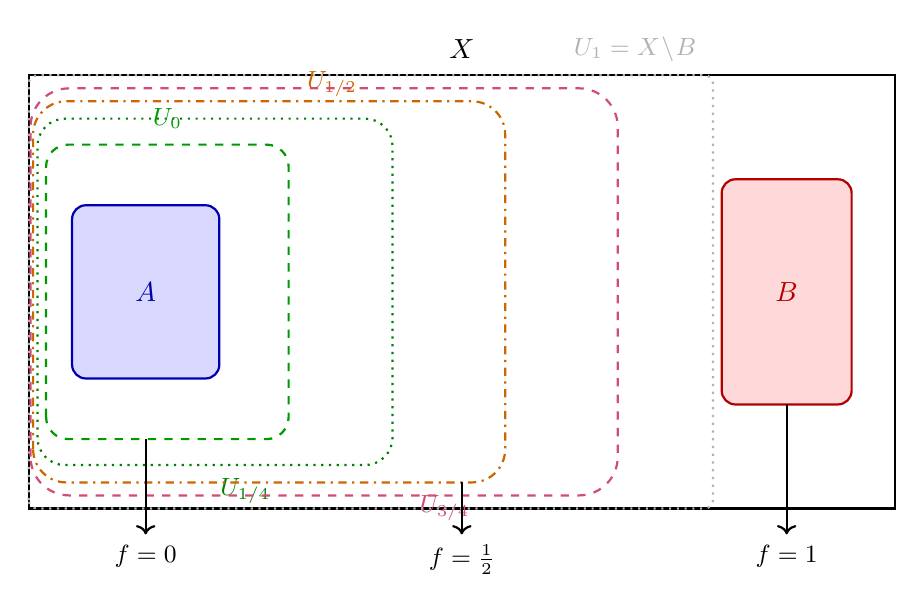
\begin{tikzpicture}[scale=1.1]
  % Outer rectangle
  \draw[thick] (0,0) rectangle (10,5);
  \node at (5,5.3) {$X$};

  % Closed sets A and B
  \filldraw[fill=blue!15, draw=blue!70!black, thick, rounded corners=5pt]
    (0.5,1.5) rectangle (2.2,3.5);
  \node[blue!70!black] at (1.35,2.5) {$A$};

  \filldraw[fill=red!15, draw=red!70!black, thick, rounded corners=5pt]
    (8.0,1.2) rectangle (9.5,3.8);
  \node[red!70!black] at (8.75,2.5) {$B$};

  % Nested open sets U_r
  \draw[green!60!black, thick, dashed, rounded corners=8pt]
    (0.2,0.8) rectangle (3.0,4.2);
  \node[green!60!black] at (1.6,4.5) {\small $U_0$};

  \draw[green!50!black, thick, dotted, rounded corners=10pt]
    (0.1,0.5) rectangle (4.2,4.5);
  \node[green!50!black] at (2.5,0.2) {\small $U_{1/4}$};

  \draw[orange!80!black, thick, dashdotted, rounded corners=12pt]
    (0.05,0.3) rectangle (5.5,4.7);
  \node[orange!80!black] at (3.5,4.9) {\small $U_{1/2}$};

  \draw[purple!70, thick, dashed, rounded corners=14pt]
    (0.02,0.15) rectangle (6.8,4.85);
  \node[purple!70] at (4.8,0.0) {\small $U_{3/4}$};

  \draw[gray!60, thick, dotted, rounded corners=3pt]
    (0.0,0.0) rectangle (7.9,5.0);
  \node[gray!60] at (7.0,5.3) {\small $U_1 = X\!\setminus\! B$};

  % Arrow showing f value
  \draw[->, thick] (1.35,0.8) -- (1.35,-0.3) node[below]{\small $f=0$};
  \draw[->, thick] (5.0,0.3) -- (5.0,-0.3) node[below]{\small $f=\tfrac{1}{2}$};
  \draw[->, thick] (8.75,1.2) -- (8.75,-0.3) node[below]{\small $f=1$};
\end{tikzpicture}
\caption{The Urysohn function construction.  The nested open sets
$U_0\subseteq U_{1/4}\subseteq U_{1/2}\subseteq U_{3/4}\subseteq U_1$
satisfy $\overline{U_r}\subseteq U_s$ for $r<s$.  The function $f$
takes value~$0$ on $A$ and value~$1$ on $B$, varying continuously
through the nested layers.}
\label{fig:urysohn-construction}
\end{figure}

\begin{corollary}
\label{cor:normal-implies-completely-regular}
\index{normal space!is completely regular}
Every normal ($T_4$) space is completely regular ($T_{3\frac{1}{2}}$).
\end{corollary}

\begin{proof}
Let $X$ be normal, $F\subseteq X$ closed, and $x\in X\setminus F$.
Since $X$ is $T_1$, the singleton $\{x\}$ is closed.  By normality,
$\{x\}$ and $F$ are disjoint closed sets, so Urysohn's lemma provides
a continuous $f\colon X\to[0,1]$ with $f(x)=0$ and $f|_F\equiv 1$.
\end{proof}

%% ----------------------------------------------------------------
\section{The Tietze Extension Theorem}
\label{sec:tietze}

\begin{theorem}[Tietze Extension Theorem]
\label{thm:tietze-extension}
\index{Tietze extension theorem!statement and proof}
Let $X$ be a normal space and $A\subseteq X$ a closed subspace.  If
$f\colon A\to[a,b]$ is continuous, then there exists a continuous
function $F\colon X\to[a,b]$ such that $F|_A = f$.
\end{theorem}

\begin{proof}
By an affine change of variables it suffices to treat the case
$[a,b]=[-1,1]$.  We construct a sequence of continuous functions
$g_n\colon X\to\mathbb{R}$ and set $F=\sum_{n=0}^{\infty}g_n$.

\medskip
\textbf{Step~1.  Iterative approximation.}
Given a continuous function $h\colon A\to[-c,c]$ (for some $c>0$) and
the normal space $X$, we show there exists a continuous function
$g\colon X\to[-c/3,\,c/3]$ such that
\begin{equation}
  \label{eq:tietze-approx}
  |h(a) - g(a)| \;\le\; \frac{2c}{3}
  \quad\text{for all }a\in A.
\end{equation}

Define
\[
  A_1 = h^{-1}\bigl([-c,\,-c/3]\bigr),\qquad
  A_2 = h^{-1}\bigl([c/3,\,c]\bigr).
\]
Since $h$ is continuous and $A$ carries the subspace topology, $A_1$
and $A_2$ are closed in $A$.  Since $A$ is closed in $X$, both $A_1$
and $A_2$ are closed in $X$.  Moreover, $A_1\cap A_2=\varnothing$.  By
Urysohn's lemma (Theorem~\ref{thm:urysohn-lemma}) there exists a
continuous function $g\colon X\to[-c/3,\,c/3]$ with $g|_{A_1}\equiv
-c/3$ and $g|_{A_2}\equiv c/3$.  (Explicitly, apply Urysohn's lemma to
obtain $\varphi\colon X\to[0,1]$ with $\varphi|_{A_1}\equiv 0$ and
$\varphi|_{A_2}\equiv 1$, then set $g = \frac{2c}{3}\varphi - \frac{c}{3}$.)

We verify~\eqref{eq:tietze-approx}.  For $a\in A_1$: $h(a)\in[-c,-c/3]$
and $g(a)=-c/3$, so $|h(a)-g(a)|\le 2c/3$.  For $a\in A_2$:
$h(a)\in[c/3,c]$ and $g(a)=c/3$, so $|h(a)-g(a)|\le 2c/3$.  For
$a\in A\setminus(A_1\cup A_2)$: $h(a)\in(-c/3,c/3)$ and
$|g(a)|\le c/3$, so $|h(a)-g(a)|< 2c/3$.

\medskip
\textbf{Step~2.  Inductive construction.}
Set $f_0=f$ (so $f_0\colon A\to[-1,1]$) and $c_0=1$.  Applying Step~1
with $h=f_0$ and $c=c_0=1$, we obtain $g_0\colon X\to[-1/3,1/3]$
such that $|f_0(a)-g_0(a)|\le 2/3$ for all $a\in A$.

Define $f_1 = f_0 - g_0|_A$; then $f_1\colon A\to[-2/3,\,2/3]$.
Apply Step~1 with $h=f_1$ and $c_1 = 2/3$ to get
$g_1\colon X\to[-(2/3)/3,\,(2/3)/3]=[-2/9,\,2/9]$ with
$|f_1(a)-g_1(a)|\le (2/3)^2$ for all $a\in A$.

Inductively, at stage $n$ we have $f_n\colon A\to[-(2/3)^n,(2/3)^n]$,
and we obtain $g_n\colon X\to[-(2/3)^n/3,\,(2/3)^n/3]$ with
$|f_n(a)-g_n(a)|\le(2/3)^{n+1}$.  Set $f_{n+1}=f_n-g_n|_A$.

\medskip
\textbf{Step~3.  Convergence and properties of $F$.}
Define
\[
  F(x) = \sum_{n=0}^{\infty} g_n(x).
\]
We have $\|g_n\|_\infty \le \frac{1}{3}\bigl(\frac{2}{3}\bigr)^n$, so
$\sum_{n=0}^{\infty}\|g_n\|_\infty = \frac{1}{3}\cdot\frac{1}
{1-2/3}=1<\infty$.  By the Weierstrass $M$-test, the series converges
uniformly on $X$, so $F$ is continuous.

Moreover, $|F(x)|\le\sum_{n=0}^{\infty}\|g_n\|_\infty = 1$, so
$F\colon X\to[-1,1]$.

Finally, for $a\in A$:
\[
  F(a) = \sum_{n=0}^{\infty}g_n(a)
       = \lim_{N\to\infty}\sum_{n=0}^{N}g_n(a).
\]
By construction, $f(a)-\sum_{n=0}^{N}g_n(a)=f_{N+1}(a)$, and
$|f_{N+1}(a)|\le(2/3)^{N+1}\to 0$.  Hence $F(a)=f(a)$ for all
$a\in A$.
\end{proof}

\begin{remark}
\label{rem:tietze-unbounded}
The Tietze extension theorem also holds for $f\colon A\to\mathbb{R}$
(unbounded case).  One may reduce to the bounded case via the
homeomorphism $\mathbb{R}\cong(-1,1)$ given by $t\mapsto t/(1+|t|)$,
or alternatively extend $f$ to a bounded function first and then
post-compose.  The resulting extension $F\colon X\to\mathbb{R}$ is
continuous.
\end{remark}

\begin{remark}
\label{rem:tietze-converse}
The converse also holds: if every continuous real-valued function on a
closed subspace of $X$ extends to $X$, then $X$ is normal.  Hence the
Tietze extension property \emph{characterizes} normality (among $T_1$
spaces).
\end{remark}

%% ----------------------------------------------------------------
\section{The Urysohn Metrization Theorem}
\label{sec:urysohn-metrization}
\index{Urysohn metrization theorem}
\index{metrization!Urysohn theorem}

\begin{theorem}[Urysohn Metrization Theorem]
\label{thm:urysohn-metrization}
Every regular\index{regular space} ($T_3$), second
countable\index{second countable} space is metrizable.
\end{theorem}

\begin{proof}
Let $X$ be a regular, second countable space with countable basis
$\mathcal{B}=\{B_n\}_{n\ge 1}$.  Recall that a regular, second
countable space is normal (a classical result).

\medskip
\textbf{Step~1.  Constructing a countable separating family of functions.}
For each pair $(m,n)$ with $\overline{B_m}\subseteq B_n$, apply
Urysohn's lemma to the disjoint closed sets $\overline{B_m}$ and
$X\setminus B_n$: there exists a continuous function
$f_{m,n}\colon X\to[0,1]$ with $f_{m,n}|_{\overline{B_m}}\equiv 1$
and $f_{m,n}|_{X\setminus B_n}\equiv 0$.  The collection
$\{f_{m,n}\}$ is countable.

\emph{This family separates points from closed sets.}  Given a closed
set $F$ and $x\notin F$, choose (by regularity) a basis element $B_n$
with $x\in B_n\subseteq X\setminus F$.  By regularity again (and
second countability), find $B_m$ with
$x\in B_m\subseteq\overline{B_m}\subseteq B_n$.  Then
$f_{m,n}(x)=1$ and $f_{m,n}|_F\equiv 0$.

\medskip
\textbf{Step~2.  Embedding in $\mathbb{R}^\omega$.}
\index{embedding!in $\mathbb{R}^\omega$}
Enumerate the family of functions as $\{f_k\}_{k\ge 1}$.  Define
$\Phi\colon X\to\mathbb{R}^\omega$ by
\[
  \Phi(x) = \bigl(f_1(x),\,f_2(x),\,f_3(x),\,\ldots\bigr).
\]
Since each $f_k$ is continuous and $\mathbb{R}^\omega$ carries the
product topology, $\Phi$ is continuous.  The separating property
ensures that $\Phi$ is injective and that $\Phi$ is an embedding
(i.e., a homeomorphism onto its image): if $U\subseteq X$ is open,
$x\in U$, then there exists $f_k$ with $f_k(x)>0$ and
$f_k|_{X\setminus U}\equiv 0$, so $\Phi(U)$ is open in
$\Phi(X)$.

\medskip
\textbf{Step~3.  Metrizability.}
The space $\mathbb{R}^\omega$ (with the product topology) is
metrizable; one compatible metric is
\[
  d\bigl((x_k),(y_k)\bigr)
  = \sum_{k=1}^{\infty}\frac{1}{2^k}\,
    \frac{|x_k - y_k|}{1+|x_k - y_k|}.
\]
Since $\Phi$ is an embedding, $X$ is homeomorphic to a subspace of a
metrizable space, hence metrizable.
\end{proof}

\begin{corollary}
\label{cor:compact-hausdorff-2nd-count-metrizable}
Every compact Hausdorff second countable space is metrizable.
\end{corollary}

\begin{proof}
A compact Hausdorff space is normal, hence regular.  Apply
Theorem~\ref{thm:urysohn-metrization}.
\end{proof}

%% ----------------------------------------------------------------
\section{Applications: Partitions of Unity}
\label{sec:partitions-of-unity}
\index{partition of unity}

\begin{definition}[Partition of unity]
\label{def:partition-of-unity}
Let $X$ be a topological space and let $\{U_\alpha\}_{\alpha\in I}$ be
an open cover of $X$.  A \textbf{partition of unity subordinate to}
$\{U_\alpha\}$ is a family $\{\varphi_\alpha\}_{\alpha\in I}$ of
continuous functions $\varphi_\alpha\colon X\to[0,1]$ such that:
\begin{enumerate}
  \item $\operatorname{supp}(\varphi_\alpha)\subseteq U_\alpha$ for each
        $\alpha\in I$;
  \item the family $\{\operatorname{supp}(\varphi_\alpha)\}$ is
        locally finite;
  \item $\sum_{\alpha\in I}\varphi_\alpha(x) = 1$ for every $x\in X$.
\end{enumerate}
\end{definition}

\begin{theorem}
\label{thm:partition-of-unity-paracompact}
\index{paracompact space!partition of unity}
A Hausdorff space $X$ is paracompact if and only if every open cover
of $X$ admits a partition of unity subordinate to it.
\end{theorem}

\begin{proof}[Proof sketch]
The ``if'' direction is straightforward: the supports give a locally
finite refinement.  For the ``only if'' direction, one uses the
shrinking lemma for locally finite covers and Urysohn's lemma on each
pair (shrunken closed set, complement of original open set) to
construct the functions, then normalizes.
\end{proof}

\begin{remark}
\label{rem:partitions-applications}
Partitions of unity are indispensable in differential geometry and the
theory of manifolds.  They allow one to pass from local constructions
(defined on coordinate charts) to global objects on the manifold---for
instance, Riemannian metrics, integration of differential forms, and
extension of sections of vector bundles.
\end{remark}

%% ----------------------------------------------------------------
\section{Counterexample: The Sorgenfrey Plane}
\label{sec:sorgenfrey-plane-not-normal}
\index{Sorgenfrey plane!non-normality}

\begin{example}
\label{ex:sorgenfrey-plane-not-normal}
The \textbf{Sorgenfrey plane}\index{Sorgenfrey plane} $S=\mathbb{R}_\ell
\times\mathbb{R}_\ell$ (the product of two copies of the Sorgenfrey
line, see Appendix~\ref{app:sorgenfrey-line}) is \emph{not} normal.

Consider the anti-diagonal $\Delta'=\{(x,-x):x\in\mathbb{R}\}$ and
its subsets $A=\{(x,-x):x\in\mathbb{Q}\}$ and
$B=\{(x,-x):x\in\mathbb{R}\setminus\mathbb{Q}\}$.  Both $A$ and $B$
are closed in $S$ (they are closed discrete subsets of the closed
subspace $\Delta'$), and $A\cap B=\varnothing$.  However, one can show
(using a Baire category argument or a cardinality argument on the
real line) that there do not exist disjoint open sets in $S$ separating
$A$ and $B$.

Since $S$ is not normal, Urysohn's lemma cannot be applied: there is
no continuous function $f\colon S\to[0,1]$ with $f|_A\equiv 0$ and
$f|_B\equiv 1$.
\end{example}

%% ----------------------------------------------------------------
\section{Worked Examples}
\label{sec:urysohn-worked-examples}

\begin{example}[Extending a continuous function]
\label{ex:tietze-worked-1}
Let $X=\mathbb{R}$ (which is normal) and $A=[0,1]\cup[2,3]$.  Define
$f\colon A\to[0,1]$ by $f(x)=x$ for $x\in[0,1]$ and $f(x)=3-x$ for
$x\in[2,3]$.  The Tietze extension theorem guarantees a continuous
extension $F\colon\mathbb{R}\to[0,1]$.  In fact, one explicit extension
is
\[
  F(x) = \begin{cases}
    x     & \text{if }x\in[0,1],\\
    1     & \text{if }x\in[1,2],\\
    3-x   & \text{if }x\in[2,3],\\
    0     & \text{if }x\notin[0,3].
  \end{cases}
\]
\end{example}

\begin{example}[Urysohn function in a metric space]
\label{ex:urysohn-metric}
In $\mathbb{R}^2$ with the Euclidean metric, let $A=\overline{B}(0,1)$
(closed unit disk) and $B=\{x\in\mathbb{R}^2:\|x\|\ge 2\}$.  An
explicit Urysohn function is
\[
  f(x)=\begin{cases}
    0              & \text{if }\|x\|\le 1,\\
    \|x\|-1        & \text{if }1\le\|x\|\le 2,\\
    1              & \text{if }\|x\|\ge 2.
  \end{cases}
\]
This is continuous, takes value $0$ on $A$ and $1$ on $B$.
\end{example}

\begin{example}[A non-extendable function on a non-normal space]
\label{ex:non-extendable}
Let $S=\mathbb{R}_\ell\times\mathbb{R}_\ell$ be the Sorgenfrey plane
and $\Delta'=\{(x,-x):x\in\mathbb{R}\}$ the anti-diagonal.  The
subspace $\Delta'$ is discrete in $S$, so \emph{every} function
$f\colon\Delta'\to\mathbb{R}$ is continuous.  However, not every such
function extends continuously to $S$.  For instance, the characteristic
function $\chi_A$ of $A=\{(q,-q):q\in\mathbb{Q}\}$ on $\Delta'$ does
not extend to a continuous function $S\to\mathbb{R}$, since $S$ is not
normal and the Tietze extension theorem fails.
\end{example}

%% ----------------------------------------------------------------
\section{Exercises}
\label{sec:urysohn-exercises}

\begin{exercise}[$\bigstar$]
\label{exo:urysohn-1}
\index{Urysohn's lemma!exercises}
Let $X$ be a normal space and let $A,B\subseteq X$ be disjoint closed
sets.  Show that there exists a continuous function $f\colon X\to[0,1]$
with $f^{-1}(\{0\})=A$ and $f^{-1}(\{1\})=B$ if and only if $A$ and
$B$ are $G_\delta$ sets.
\end{exercise}

\begin{exercise}[$\bigstar$]
\label{exo:urysohn-2}
Prove that every metrizable space is completely regular directly
(without using Urysohn's lemma), using the distance function.
\end{exercise}

\begin{exercise}[$\bigstar$]
\label{exo:urysohn-3}
Let $X$ be a compact Hausdorff space.  Show that $X$ is metrizable if
and only if $X$ is second countable.
\end{exercise}

\begin{exercise}[$\bigstar\bigstar$]
\label{exo:urysohn-4}
Let $X$ be a normal space, $A\subseteq X$ closed, and
$f\colon A\to\mathbb{R}$ continuous (unbounded).  Prove that $f$
extends to a continuous function $F\colon X\to\mathbb{R}$.
\textit{Hint:} compose with a homeomorphism $\mathbb{R}\cong(-1,1)$.
\end{exercise}

\begin{exercise}[$\bigstar\bigstar$]
\label{exo:urysohn-5}
Let $X$ be a second countable, regular space.  Show that $X$ embeds in
the Hilbert cube $[0,1]^{\mathbb{N}}$.
\end{exercise}

\begin{exercise}[$\bigstar\bigstar$]
\label{exo:urysohn-6}
Show that a compact Hausdorff space $X$ is normal.  Deduce that
Urysohn's lemma and the Tietze extension theorem apply to every
compact Hausdorff space.
\end{exercise}

\begin{exercise}[$\bigstar\bigstar\bigstar$]
\label{exo:urysohn-7}
\index{Sorgenfrey plane!exercises}
Prove in detail that the Sorgenfrey plane is not normal.
\textit{Hint:} use the Jones lemma: if $X$ is normal and has a closed
discrete subspace $D$ and a dense subspace $S$, then
$2^{|D|}\le 2^{|S|}$.
\end{exercise}

\begin{exercise}[$\bigstar\bigstar\bigstar$]
\label{exo:urysohn-8}
\index{partition of unity!construction}
Let $X$ be a normal space and $\{U_1,U_2\}$ a finite open cover.
Construct an explicit partition of unity $\{\varphi_1,\varphi_2\}$
subordinate to this cover using Urysohn's lemma.  Generalize to a
finite open cover $\{U_1,\ldots,U_n\}$.
\end{exercise}

%% ----------------------------------------------------------------
\section*{Chapter Summary}

\begin{itemize}
  \item A space is \textbf{completely regular} ($T_{3\frac{1}{2}}$) if
        points can be separated from closed sets by continuous functions
        into $[0,1]$.
  \item \textbf{Urysohn's lemma:} in a normal space, disjoint closed
        sets can be separated by a continuous function $f\colon X\to[0,1]$.
        The proof constructs nested open sets indexed by dyadic rationals.
  \item \textbf{Tietze extension theorem:} in a normal space, every
        continuous function $f\colon A\to[a,b]$ on a closed subspace $A$
        extends to a continuous function $F\colon X\to[a,b]$.  The proof
        uses an iterative approximation based on Urysohn's lemma.
  \item The \textbf{Urysohn metrization theorem} states that every
        regular, second countable space is metrizable, via embedding in
        $\mathbb{R}^\omega$.
  \item \textbf{Partitions of unity} subordinate to open covers exist
        for paracompact Hausdorff spaces and are essential tools in
        analysis and geometry.
  \item The Sorgenfrey plane provides a key counterexample: it is
        separable and first countable, but not normal.
\end{itemize}

\index{Urysohn's lemma|)}
\index{Tietze extension theorem|)}


%% ================================================================
%%  CHAPTER 10 — A Preview of Algebraic Topology
%% ================================================================
\chapter{A Preview of Algebraic Topology}
\label{ch:algebraic-topology}
\index{algebraic topology|(}

\section*{Motivation}

Throughout this course, we have classified topological spaces using
properties such as compactness, connectedness, and separation axioms.
Yet these properties are often insufficient to distinguish between
spaces that are intuitively very different.  For example, both
$\mathbb{R}^2$ and $\mathbb{R}^2\setminus\{0\}$ are connected, locally
compact, Hausdorff, and metrizable---yet they are not homeomorphic.
How can we prove this?

The key insight, due to Poincar\'{e}\index{Poincar\'e, Henri}, is to
assign \emph{algebraic invariants}---groups, rings, modules---to
topological spaces in such a way that homeomorphic spaces receive
isomorphic invariants.  This is the domain of \textbf{algebraic
topology}, and it transforms topological questions into algebraic
computations.  In this chapter, we give a brief, self-contained preview
of the main ideas: homotopy, the fundamental group, covering spaces,
and some spectacular applications.

%% ----------------------------------------------------------------
\section{Homotopy}
\label{sec:homotopy}
\index{homotopy|(}

\begin{definition}[Homotopy of maps]
\label{def:homotopy}
\index{homotopy!of maps}
Let $X$ and $Y$ be topological spaces and let $f,g\colon X\to Y$ be
continuous maps.  A \textbf{homotopy} from $f$ to $g$ is a continuous
map $H\colon X\times[0,1]\to Y$ such that
\[
  H(x,0) = f(x) \quad\text{and}\quad H(x,1)=g(x)
  \qquad\text{for all }x\in X.
\]
If such an $H$ exists, we say $f$ and $g$ are \textbf{homotopic} and
write $f\simeq g$.
\end{definition}

\begin{proposition}
\label{prop:homotopy-equivalence-relation}
Homotopy is an equivalence relation on the set of continuous maps from
$X$ to $Y$.
\end{proposition}

\begin{proof}
\emph{Reflexivity:} $H(x,t)=f(x)$ for all $t$.
\emph{Symmetry:} if $H$ is a homotopy from $f$ to $g$, then
$\overline{H}(x,t)=H(x,1-t)$ is a homotopy from $g$ to $f$.
\emph{Transitivity:} if $H_1\colon f\simeq g$ and $H_2\colon g\simeq h$,
define
\[
  H(x,t) = \begin{cases}
    H_1(x,2t)   & \text{if }t\in[0,\tfrac{1}{2}],\\
    H_2(x,2t-1) & \text{if }t\in[\tfrac{1}{2},1].
  \end{cases}
\]
By the pasting lemma, $H$ is continuous.
\end{proof}

\begin{definition}[Homotopy equivalence]
\label{def:homotopy-equivalence}
\index{homotopy!equivalence}
Spaces $X$ and $Y$ are \textbf{homotopy equivalent} (or have the same
\textbf{homotopy type}), written $X\simeq Y$, if there exist continuous
maps $f\colon X\to Y$ and $g\colon Y\to X$ such that $g\circ f\simeq
\mathrm{id}_X$ and $f\circ g\simeq\mathrm{id}_Y$.
\end{definition}

\begin{definition}[Deformation retract]
\label{def:deformation-retract}
\index{deformation retract}
A subspace $A\subseteq X$ is a \textbf{deformation retract} of $X$ if
there exists a continuous map $H\colon X\times[0,1]\to X$ such that
$H(x,0)=x$, $H(x,1)\in A$ for all $x\in X$, and $H(a,t)=a$ for all
$a\in A$ and $t\in[0,1]$.  In this case, $X\simeq A$.
\end{definition}

\begin{example}
\label{ex:deformation-retracts}
\begin{enumerate}
  \item $\mathbb{R}^n\setminus\{0\}$ deformation-retracts onto
        $S^{n-1}$ via $H(x,t) = (1-t)x + t\cdot\frac{x}{\|x\|}$.
  \item The M\"obius band deformation-retracts onto its central circle.
  \item Any convex subset of $\mathbb{R}^n$ is contractible (homotopy
        equivalent to a point).
\end{enumerate}
\end{example}

\begin{figure}[ht]
\centering
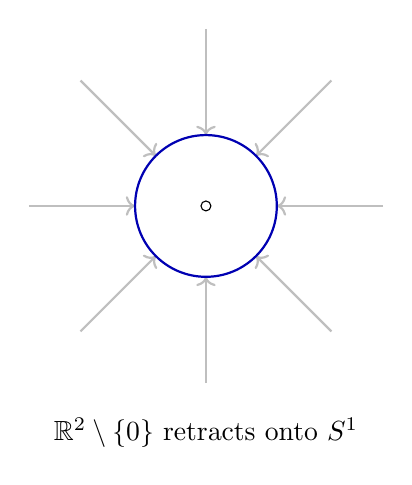
\begin{tikzpicture}[scale=0.9]
  % Deformation retract of R^2\{0} onto S^1
  \draw[->, thick, gray!50] (2.5,0) -- (1,0);
  \draw[->, thick, gray!50] (0,2.5) -- (0,1);
  \draw[->, thick, gray!50] (-2.5,0) -- (-1,0);
  \draw[->, thick, gray!50] (0,-2.5) -- (0,-1);
  \draw[->, thick, gray!50] (1.77,1.77) -- (0.707,0.707);
  \draw[->, thick, gray!50] (-1.77,1.77) -- (-0.707,0.707);
  \draw[->, thick, gray!50] (1.77,-1.77) -- (0.707,-0.707);
  \draw[->, thick, gray!50] (-1.77,-1.77) -- (-0.707,-0.707);
  \draw[thick, blue!70!black] (0,0) circle (1);
  \filldraw[white] (0,0) circle (0.07);
  \draw (0,0) circle (0.07);
  \node at (0,-3.2) {$\mathbb{R}^2\setminus\{0\}$ retracts onto $S^1$};
\end{tikzpicture}
\caption{The deformation retract of $\mathbb{R}^2\setminus\{0\}$ onto
$S^1$: each point moves radially towards the unit circle.}
\label{fig:deformation-retract}
\end{figure}

\index{homotopy|)}

%% ----------------------------------------------------------------
\section{The Fundamental Group}
\label{sec:fundamental-group}
\index{fundamental group|(}

\begin{definition}[Loop and fundamental group]
\label{def:fundamental-group}
Let $X$ be a topological space and $x_0\in X$ a \textbf{basepoint}\index{basepoint}.
A \textbf{loop}\index{loop} based at $x_0$ is a continuous map
$\gamma\colon[0,1]\to X$ with $\gamma(0)=\gamma(1)=x_0$.  Two loops
$\gamma$ and $\delta$ are \textbf{path-homotopic}\index{path homotopy}
if there exists a continuous map $H\colon[0,1]\times[0,1]\to X$ with
$H(s,0)=\gamma(s)$, $H(s,1)=\delta(s)$, and $H(0,t)=H(1,t)=x_0$
for all $s,t$.

The \textbf{fundamental group}\index{fundamental group!definition} of
$X$ at $x_0$ is the set of path-homotopy classes of loops based at
$x_0$:
\[
  \pi_1(X,x_0) = \{[\gamma] : \gamma\text{ is a loop at }x_0\},
\]
equipped with the group operation given by concatenation of loops:
\[
  ([\gamma]\cdot[\delta])(s) = \begin{cases}
    \gamma(2s)   & \text{if }s\in[0,\tfrac{1}{2}],\\
    \delta(2s-1) & \text{if }s\in[\tfrac{1}{2},1].
  \end{cases}
\]
The identity element is the class of the constant loop at $x_0$, and
the inverse of $[\gamma]$ is $[\bar{\gamma}]$ where
$\bar{\gamma}(s)=\gamma(1-s)$.
\end{definition}

\begin{theorem}
\label{thm:pi1-well-defined}
$\pi_1(X,x_0)$ is a group under the concatenation operation.
\end{theorem}

\begin{proof}[Proof sketch]
One must verify that concatenation is well-defined on homotopy classes
(if $\gamma\simeq\gamma'$ and $\delta\simeq\delta'$, then
$\gamma*\delta\simeq\gamma'*\delta'$), associative up to homotopy,
and that the constant loop and reversal of loops provide identity and
inverses.  Each verification amounts to constructing an explicit
homotopy by reparametrizing the interval $[0,1]$.
\end{proof}

\begin{theorem}
\label{thm:pi1-topological-invariant}
\index{fundamental group!topological invariant}
If $f\colon X\to Y$ is a homeomorphism with $f(x_0)=y_0$, then
$\pi_1(X,x_0)\cong\pi_1(Y,y_0)$.  More generally, if $X\simeq Y$
(homotopy equivalence), then $\pi_1(X,x_0)\cong\pi_1(Y,y_0)$ (for
appropriate basepoints).  Hence the fundamental group is a
\textbf{topological invariant}, and more generally, a \textbf{homotopy
invariant}.
\end{theorem}

\begin{proof}[Proof sketch]
A homeomorphism $f$ induces a group isomorphism $f_*\colon\pi_1(X,x_0)
\to\pi_1(Y,y_0)$ by $f_*([\gamma])=[f\circ\gamma]$.  For homotopy
equivalences, one shows that the induced map $f_*$ has an inverse
$(g\circ f\simeq\mathrm{id}$ implies $g_*\circ f_* = \mathrm{id}$
up to a change-of-basepoint isomorphism).
\end{proof}

\begin{definition}[Simply connected space]
\label{def:simply-connected}
\index{simply connected}
A path-connected space $X$ is \textbf{simply connected} if
$\pi_1(X,x_0)$ is trivial (i.e., $\pi_1(X,x_0)\cong\{e\}$) for some
(hence every) basepoint $x_0$.
\end{definition}

\begin{example}
\label{ex:simply-connected}
\begin{enumerate}
  \item $\mathbb{R}^n$ is simply connected for all $n\ge 1$: every loop
        is homotopic to a constant via the straight-line homotopy
        $H(s,t)=(1-t)\gamma(s)+t\cdot x_0$.
  \item $S^n$ is simply connected for $n\ge 2$.  (This requires a more
        careful argument using the Lebesgue number lemma.)
  \item The torus $T^2=S^1\times S^1$ is \emph{not} simply connected:
        $\pi_1(T^2)\cong\mathbb{Z}\times\mathbb{Z}$.
\end{enumerate}
\end{example}

%% ----------------------------------------------------------------
\section{The Fundamental Group of the Circle}
\label{sec:pi1-circle}
\index{fundamental group!of $S^1$}

\begin{theorem}
\label{thm:pi1-circle}
$\pi_1(S^1, 1) \cong \mathbb{Z}$.
\end{theorem}

The integer associated to a loop $\gamma$ is its \textbf{winding
number}\index{winding number}: the number of times $\gamma$ winds
around the circle, counted with sign.

\begin{proof}[Proof sketch via covering spaces]
Consider the covering map\index{covering map} $p\colon\mathbb{R}\to S^1$
defined by $p(t)=e^{2\pi it}$ (or equivalently,
$p(t)=(\cos 2\pi t,\sin 2\pi t)$).  The key facts are:

\begin{enumerate}
  \item \textbf{Path lifting:}\index{path lifting} every loop
        $\gamma\colon[0,1]\to S^1$ with $\gamma(0)=1$ lifts uniquely to
        a path $\tilde{\gamma}\colon[0,1]\to\mathbb{R}$ with
        $\tilde{\gamma}(0)=0$.  Then $\tilde{\gamma}(1)\in\mathbb{Z}$
        (since $p(\tilde{\gamma}(1))=\gamma(1)=1$).
  \item \textbf{Homotopy lifting:}\index{homotopy lifting} if
        $\gamma\simeq\delta$ (as loops at $1$), then their lifts have
        the same endpoint: $\tilde{\gamma}(1)=\tilde{\delta}(1)$.
\end{enumerate}

The map $\Phi\colon\pi_1(S^1,1)\to\mathbb{Z}$ defined by
$\Phi([\gamma])=\tilde{\gamma}(1)$ is therefore well-defined.  One
verifies that $\Phi$ is a group homomorphism (lifting of a
concatenation corresponds to addition of endpoints) and a bijection
(the loop $\gamma_n(s)=e^{2\pi i n s}$ has winding number $n$, so
$\Phi$ is surjective; and a loop with winding number~$0$ lifts to a
closed path in~$\mathbb{R}$, which is null-homotopic since
$\mathbb{R}$ is simply connected, so $\Phi$ is injective).
\end{proof}

\begin{figure}[ht]
\centering
\begin{tikzpicture}[scale=1.0]
  % The circle S^1
  \draw[thick, blue!70!black] (0,0) circle (1.5);
  \filldraw[blue!70!black] (1.5,0) circle (0.06) node[right]{\small $1$};
  \node[blue!70!black] at (0,-2.1) {$S^1$};

  % Arrow for covering map
  \draw[->, thick] (3.5,1) -- (2.3,0.3);
  \node at (3.4,0.5) {\small $p$};

  % The helix (covering space R)
  \begin{scope}[xshift=6cm, yshift=-0.5cm]
    \draw[thick, ->] (0,0) -- (0,4) node[above]{\small $\mathbb{R}$};
    % Helix projection
    \foreach \k in {0,1,2} {
      \filldraw[red!70!black] (0, \k*1.2) circle (0.05);
      \node[right, red!70!black] at (0.1, \k*1.2) {\small $\k$};
    }
    % Path lifting illustration
    \draw[thick, red!70!black, decorate, decoration={snake, amplitude=1.5mm,
      segment length=5mm}]
      (0,0) -- (0,1.2);
    \node[red!70!black] at (0.9, 0.6) {\small $\tilde{\gamma}$};
    \node at (0,-0.8) {Lift to $\mathbb{R}$};
  \end{scope}
\end{tikzpicture}
\caption{The covering space $p\colon\mathbb{R}\to S^1$.  A loop on
$S^1$ lifts to a path in $\mathbb{R}$; the endpoint of the lift is
the winding number.}
\label{fig:covering-circle}
\end{figure}

%% ----------------------------------------------------------------
\section{Covering Spaces}
\label{sec:covering-spaces}
\index{covering space|(}

\begin{definition}[Covering space]
\label{def:covering-space}
A \textbf{covering space}\index{covering space!definition} of a
topological space $X$ is a space $\tilde{X}$ together with a surjective
continuous map $p\colon\tilde{X}\to X$ (the \textbf{covering map}) such
that for every $x\in X$ there exists an open neighbourhood $U$ of $x$
with the property that $p^{-1}(U)$ is a disjoint union of open sets in
$\tilde{X}$, each of which is mapped homeomorphically onto $U$ by $p$.
Such a $U$ is called \textbf{evenly covered}\index{evenly covered}.
\end{definition}

\begin{example}
\label{ex:covering-spaces}
\begin{enumerate}
  \item $p\colon\mathbb{R}\to S^1$, $p(t)=e^{2\pi it}$, is the
        universal covering of the circle.
  \item $p\colon S^n\to\mathbb{R}P^n$ (the quotient by the antipodal
        map) is a double covering for $n\ge 1$.
  \item $p\colon\mathbb{R}^2\to T^2$ given by the quotient
        $\mathbb{R}^2/\mathbb{Z}^2$ is the universal covering of the
        torus.
\end{enumerate}
\end{example}

\begin{theorem}[Path Lifting Lemma]
\label{thm:path-lifting}
\index{path lifting}
Let $p\colon\tilde{X}\to X$ be a covering map, $\gamma\colon[0,1]\to X$
a path, and $\tilde{x}_0\in p^{-1}(\gamma(0))$.  Then there exists a
unique path $\tilde{\gamma}\colon[0,1]\to\tilde{X}$ with
$\tilde{\gamma}(0)=\tilde{x}_0$ and $p\circ\tilde{\gamma}=\gamma$.
\end{theorem}

\begin{theorem}[Homotopy Lifting Lemma]
\label{thm:homotopy-lifting}
\index{homotopy lifting}
Let $p\colon\tilde{X}\to X$ be a covering map,
$H\colon[0,1]\times[0,1]\to X$ a homotopy with $H(0,t)=x_0$ and
$H(1,t)=x_1$ for all $t$, and $\tilde{x}_0\in p^{-1}(x_0)$.  Then
$H$ lifts to a unique homotopy
$\tilde{H}\colon[0,1]\times[0,1]\to\tilde{X}$ with
$\tilde{H}(0,0)=\tilde{x}_0$ and $p\circ\tilde{H}=H$.  In particular,
$\tilde{H}(1,t)$ is independent of $t$.
\end{theorem}

\index{covering space|)}

%% ----------------------------------------------------------------
\section{The Brouwer Fixed Point Theorem}
\label{sec:brouwer}
\index{Brouwer fixed point theorem|(}

\begin{theorem}[Brouwer Fixed Point Theorem, dimension 2]
\label{thm:brouwer-fixed-point}
Every continuous map $f\colon D^2\to D^2$ has a fixed point, where
$D^2=\{x\in\mathbb{R}^2:\|x\|\le 1\}$ is the closed unit disk.
\end{theorem}

\begin{proof}
We proceed by contradiction.  Suppose $f\colon D^2\to D^2$ is
continuous with no fixed point, i.e., $f(x)\neq x$ for all $x\in D^2$.

\textbf{Step~1.  Constructing a retraction.}
For each $x\in D^2$, consider the ray starting at $f(x)$ and passing
through $x$.  Since $f(x)\neq x$, this ray is well-defined.  Let
$r(x)$ be the point where this ray intersects the boundary circle
$S^1=\partial D^2$.  Explicitly, write $r(x) = x + t(x-f(x))$ for
the unique $t\ge 0$ such that $\|r(x)\|=1$.  Standard arguments show
that $r\colon D^2\to S^1$ is continuous.

Moreover, if $x\in S^1$ already, then since $\|x\|=1$, we have
$r(x)=x$ (one can verify this directly, or note that the ray from
$f(x)\in D^2$ through $x\in S^1$ hits $S^1$ first at $x$ itself when
$t=0$).  Hence $r$ is a \textbf{retraction}\index{retraction} of $D^2$
onto $S^1$: $r|_{S^1}=\mathrm{id}_{S^1}$.

\textbf{Step~2.  Deriving a contradiction via $\pi_1$.}
Let $\iota\colon S^1\hookrightarrow D^2$ be the inclusion.  Then
$r\circ\iota = \mathrm{id}_{S^1}$, so the induced homomorphisms
satisfy
\[
  r_* \circ \iota_* = (\mathrm{id}_{S^1})_*
  = \mathrm{id}_{\pi_1(S^1)}.
\]
In particular, $\iota_*\colon\pi_1(S^1)\to\pi_1(D^2)$ is injective.
But $\pi_1(S^1)\cong\mathbb{Z}$ (Theorem~\ref{thm:pi1-circle}) and
$\pi_1(D^2)\cong\{0\}$ (since $D^2$ is convex, hence contractible).
An injective homomorphism $\mathbb{Z}\hookrightarrow\{0\}$ is
impossible.  Contradiction.
\end{proof}

\begin{remark}
\label{rem:brouwer-higher-dim}
The Brouwer fixed point theorem holds in all dimensions: every
continuous map $f\colon D^n\to D^n$ has a fixed point.  For $n\ge 3$,
the proof requires either singular homology or higher homotopy groups,
as $\pi_1(S^n)$ is trivial for $n\ge 2$.
\end{remark}

\index{Brouwer fixed point theorem|)}

%% ----------------------------------------------------------------
\section{The Borsuk--Ulam Theorem}
\label{sec:borsuk-ulam}
\index{Borsuk--Ulam theorem}

\begin{theorem}[Borsuk--Ulam, dimension 2]
\label{thm:borsuk-ulam}
For every continuous map $f\colon S^2\to\mathbb{R}^2$, there exists a
point $x\in S^2$ such that $f(x)=f(-x)$.
\end{theorem}

\begin{remark}
\label{rem:borsuk-ulam-interpretation}
Informally, at any given moment there exist two antipodal points on the
surface of the Earth that have exactly the same temperature and the same
atmospheric pressure.  This striking result generalizes to $S^n$ and
$\mathbb{R}^n$ for all $n$, and has applications in combinatorics (the
ham sandwich theorem\index{ham sandwich theorem}) and in
geometry.
\end{remark}

%% ----------------------------------------------------------------
\section{Higher Invariants: A Brief Glimpse}
\label{sec:higher-invariants}
\index{higher homotopy groups}
\index{singular homology}
\index{Euler characteristic}

The fundamental group is only the first of a family of algebraic
invariants:

\begin{itemize}
  \item \textbf{Higher homotopy groups}\index{homotopy group!higher}
        $\pi_n(X,x_0)$, $n\ge 2$, are defined using maps
        $S^n\to X$.  They are always abelian for $n\ge 2$.
  \item \textbf{Singular homology groups}\index{homology!singular}
        $H_n(X;\mathbb{Z})$ measure ``$n$-dimensional holes'' in $X$.
        For instance, $H_1(S^1)\cong\mathbb{Z}$ reflects the single
        hole enclosed by the circle, while
        $H_n(S^n)\cong\mathbb{Z}$ for all $n$.
  \item The \textbf{Euler characteristic}\index{Euler characteristic}
        $\chi(X)=\sum_{n}(-1)^n\operatorname{rank}H_n(X)$ is a
        numerical invariant.  For a closed orientable surface of genus
        $g$, $\chi=2-2g$.
\end{itemize}

The algebraization of homology---passing from Betti numbers to actual
groups---was accomplished by Emmy Noether\index{Noether, Emmy} in the
1920s, a breakthrough that shaped modern algebraic topology.

\begin{figure}[ht]
\centering
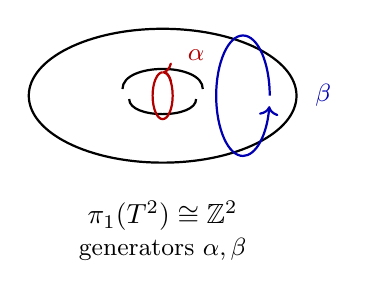
\begin{tikzpicture}[scale=0.85]
  % Torus with two loops
  \begin{scope}[xshift=0cm]
    % Outer ellipse
    \draw[thick] (0,0) ellipse (2 and 1);
    % Inner hole
    \draw[thick] (-0.6,0.1) .. controls (-0.6,0.5) and (0.6,0.5) .. (0.6,0.1);
    \draw[thick] (-0.5,-0.05) .. controls (-0.5,-0.35) and (0.5,-0.35) .. (0.5,-0.05);
    % Loop alpha (around hole)
    \draw[thick, red!70!black, ->] (0,0.35) arc (90:450:0.15 and 0.35);
    \node[red!70!black] at (0.5,0.6) {\small $\alpha$};
    % Loop beta (around tube)
    \draw[thick, blue!70!black, ->] (1.6,0) arc (0:350:0.4 and 0.9);
    \node[blue!70!black] at (2.4,0) {\small $\beta$};
    \node at (0,-1.8) {$\pi_1(T^2)\cong\mathbb{Z}^2$};
    \node at (0,-2.3) {\small generators $\alpha,\beta$};
  \end{scope}
\end{tikzpicture}
\caption{Two generating loops on the torus $T^2 = S^1\times S^1$.  The
fundamental group is $\pi_1(T^2)\cong\mathbb{Z}\times\mathbb{Z}$,
generated by the loops $\alpha$ (around the hole) and $\beta$ (around
the tube).}
\label{fig:torus-loops}
\end{figure}

%% ----------------------------------------------------------------
\section{Historical Notes}
\label{sec:algebraic-topology-history}

\begin{itemize}
  \item \textbf{Henri Poincar\'{e}}\index{Poincar\'e, Henri} (1895)
        introduced the fundamental group and homology in his landmark
        paper \emph{Analysis Situs}, founding algebraic topology.
  \item \textbf{L.~E.~J.\ Brouwer}\index{Brouwer, L.~E.~J.} (1911)
        proved his fixed point theorem and the invariance of domain,
        using simplicial methods.
  \item \textbf{Emmy Noether}\index{Noether, Emmy} (1925--1930)
        recognized that homology should be formulated in terms of
        groups and homomorphisms rather than mere numerical invariants
        (Betti numbers and torsion coefficients), thereby laying the
        algebraic foundations of the subject.
  \item The modern axiomatic approach to homology was developed by
        \textbf{Eilenberg} and \textbf{Steenrod}\index{Eilenberg--Steenrod axioms}
        (1945), culminating in their book \emph{Foundations of Algebraic
        Topology} (1952).
\end{itemize}

%% ----------------------------------------------------------------
\section{Exercises}
\label{sec:algtop-exercises}

\begin{exercise}[$\bigstar$]
\label{exo:algtop-1}
Show that homotopy equivalence is an equivalence relation on topological
spaces.
\end{exercise}

\begin{exercise}[$\bigstar$]
\label{exo:algtop-2}
\index{contractible space}
A space $X$ is \textbf{contractible} if it is homotopy equivalent to a
point.  Show that every convex subset of $\mathbb{R}^n$ is contractible.
\end{exercise}

\begin{exercise}[$\bigstar\bigstar$]
\label{exo:algtop-3}
Let $X$ be path-connected and let $x_0,x_1\in X$.  Show that
$\pi_1(X,x_0)\cong\pi_1(X,x_1)$.
\textit{Hint:} use a path from $x_0$ to $x_1$ to construct the
isomorphism.
\end{exercise}

\begin{exercise}[$\bigstar\bigstar$]
\label{exo:algtop-4}
Compute $\pi_1(S^1\vee S^1)$, where $S^1\vee S^1$ is the wedge
(one-point union) of two circles.
\textit{Answer:} the free group on two generators, $F_2$.
\end{exercise}

\begin{exercise}[$\bigstar\bigstar$]
\label{exo:algtop-5}
Use the Brouwer fixed point theorem to prove the following: for every
continuous function $f\colon[0,1]\to[0,1]$, there exists $x\in[0,1]$
with $f(x)=x$.  (Give a direct proof from the intermediate value
theorem as well.)
\end{exercise}

\begin{exercise}[$\bigstar\bigstar\bigstar$]
\label{exo:algtop-6}
\index{fundamental theorem of algebra}
Use the fundamental group to prove the \textbf{fundamental theorem of
algebra}: every non-constant polynomial $p(z)\in\mathbb{C}[z]$ has a
root in $\mathbb{C}$.
\textit{Hint:} consider the map $\gamma_R(t) = p(Re^{2\pi it})/
|p(Re^{2\pi it})|$ from $S^1$ to $S^1$ for large $R$, and show its
winding number equals $\deg p$.
\end{exercise}

%% ----------------------------------------------------------------
\section*{Chapter Summary}

\begin{itemize}
  \item \textbf{Homotopy} formalizes the idea of continuous deformation
        of maps.  \textbf{Homotopy equivalence} is a coarser relation
        than homeomorphism but preserves algebraic invariants.
  \item The \textbf{fundamental group} $\pi_1(X,x_0)$ consists of
        homotopy classes of loops at a basepoint, and is a topological
        (and homotopy) invariant.
  \item $\pi_1(S^1)\cong\mathbb{Z}$, proved via the covering space
        $\mathbb{R}\to S^1$.  A \textbf{simply connected} space has
        trivial fundamental group.
  \item The \textbf{Brouwer fixed point theorem} (dimension~2) states
        that every continuous self-map of the closed disk has a fixed
        point; its proof uses $\pi_1$.
  \item \textbf{Covering spaces} provide the key technical tool:
        path lifting and homotopy lifting.
  \item Algebraic topology offers a wealth of further invariants:
        higher homotopy groups, homology, cohomology, and the Euler
        characteristic.
\end{itemize}

\section*{Concluding Remarks: Where to Go from Here}

This course has taken us from the bare axioms of a topological space
through compactness, connectedness, separation, and metrization, all
the way to the threshold of algebraic topology.  We close with a brief
guide to further study.

\begin{itemize}
  \item \textbf{Algebraic topology.}  A full treatment of the
        fundamental group, covering space theory, singular homology and
        cohomology, and their applications.  The standard reference is
        Hatcher~\cite{hatcher}.
  \item \textbf{Differential topology.}  The study of smooth manifolds,
        tangent bundles, transversality, and degree theory.  Milnor's
        \emph{Topology from the Differentiable Viewpoint} is an
        excellent starting point.
  \item \textbf{Geometric topology.}  Classification of surfaces,
        3-manifold theory (including Thurston's geometrization and the
        Poincar\'{e} conjecture, proved by Perelman in 2003), knot theory,
        and 4-manifold theory.
  \item \textbf{Functional analysis and descriptive set theory.}  Many
        results from general topology---Tychonoff's theorem, the
        Baire category theorem, Urysohn's lemma---find deep
        applications in the study of Banach spaces, operator algebras,
        and the structure of Borel and analytic sets.
\end{itemize}

\index{algebraic topology|)}


%% ================================================================
%%  APPENDIX A — Catalogue of Counterexamples
%% ================================================================
\appendix
\chapter{Catalogue of Counterexamples}
\label{app:counterexamples}
\index{counterexamples|(}

The following spaces are standard sources of counterexamples in general
topology.  For each, we give the definition, the key properties, and
the theorems it illuminates.

%% ----------------------------------------------------------------
\section{The Sorgenfrey Line}
\label{app:sorgenfrey-line}
\index{Sorgenfrey line|(}

\textbf{Definition.}
Let $\mathbb{R}_\ell$ denote the real line equipped with the
\emph{lower limit topology} (or \emph{half-open interval topology}):
the topology generated by the basis $\{[a,b) : a<b,\; a,b\in\mathbb{R}\}$.

\medskip
\textbf{Key properties.}
\begin{itemize}
  \item $T_1$: yes. \quad $T_2$ (Hausdorff): yes. \quad $T_3$ (regular): yes. \quad $T_4$ (normal): yes.
  \item Completely regular ($T_{3\frac{1}{2}}$): yes.
  \item Separable: yes ($\mathbb{Q}$ is dense).
  \item First countable: yes. \quad Second countable: \textbf{no}.
  \item Lindel\"of: yes.
  \item Compact: \textbf{no}. \quad Locally compact: \textbf{no}.
  \item Connected: \textbf{no} (totally disconnected).
  \item Metrizable: \textbf{no} (separable but not second countable).
  \item Paracompact: yes.
\end{itemize}

\textbf{Counterexamples provided.}
\begin{enumerate}
  \item A separable space need not be second countable.
  \item A normal, separable space need not be metrizable (refutes the
        converse of the Urysohn metrization theorem without the second
        countability hypothesis).
  \item A Lindel\"of space need not be second countable.
\end{enumerate}
\index{Sorgenfrey line|)}

%% ----------------------------------------------------------------
\section{The Sorgenfrey Plane}
\label{app:sorgenfrey-plane}
\index{Sorgenfrey plane|(}

\textbf{Definition.}
$S = \mathbb{R}_\ell \times \mathbb{R}_\ell$, the product of two
copies of the Sorgenfrey line, with the product topology.

\medskip
\textbf{Key properties.}
\begin{itemize}
  \item $T_1$: yes. \quad $T_2$: yes. \quad $T_3$: yes. \quad $T_{3\frac{1}{2}}$: yes.
  \item $T_4$ (normal): \textbf{no}.
  \item Separable: yes ($\mathbb{Q}^2$ is dense). \quad First countable: yes. \quad Second countable: \textbf{no}.
  \item Lindel\"of: \textbf{no}. \quad Compact: \textbf{no}.
  \item Metrizable: \textbf{no}. \quad Paracompact: \textbf{no}.
\end{itemize}

\textbf{Counterexamples provided.}
\begin{enumerate}
  \item The product of two normal spaces need not be normal.
  \item The product of two Lindel\"of spaces need not be Lindel\"of.
  \item The product of two paracompact spaces need not be paracompact.
  \item A separable, first countable, completely regular space need not
        be normal.
  \item Urysohn's lemma and the Tietze extension theorem fail in
        non-normal spaces (see Example~\ref{ex:sorgenfrey-plane-not-normal}).
\end{enumerate}
\index{Sorgenfrey plane|)}

%% ----------------------------------------------------------------
\section{Cofinite Topology on an Infinite Set}
\label{app:cofinite}
\index{cofinite topology|(}

\textbf{Definition.}
Let $X$ be an infinite set.  The \emph{cofinite topology} (or
\emph{finite complement topology}) on $X$ consists of $\varnothing$
and all subsets whose complement is finite.

\medskip
\textbf{Key properties.}
\begin{itemize}
  \item $T_0$: yes. \quad $T_1$: yes. \quad $T_2$ (Hausdorff): \textbf{no}
        (any two non-empty open sets intersect).
  \item Compact: yes (every open cover has a finite subcover, since
        removing one open set leaves only finitely many points to cover).
  \item Connected: yes (no proper non-empty clopen set exists).
  \item Second countable: yes if $X$ is countable; no if $X$ is
        uncountable.
  \item Metrizable: \textbf{no} (not Hausdorff).
\end{itemize}

\textbf{Counterexamples provided.}
\begin{enumerate}
  \item A compact, $T_1$ space need not be Hausdorff.
  \item A compact space need not be metrizable.
  \item Limits of sequences are not unique in non-Hausdorff spaces.
\end{enumerate}
\index{cofinite topology|)}

%% ----------------------------------------------------------------
\section{Cocountable Topology on an Uncountable Set}
\label{app:cocountable}
\index{cocountable topology|(}

\textbf{Definition.}
Let $X$ be an uncountable set.  The \emph{cocountable topology} on $X$
consists of $\varnothing$ and all subsets whose complement is countable.

\medskip
\textbf{Key properties.}
\begin{itemize}
  \item $T_0$: yes. \quad $T_1$: yes. \quad $T_2$: \textbf{no}.
  \item Compact: \textbf{no} (if $X$ is uncountable; consider a
        partition into uncountably many singletons---though singletons
        are not open.  More carefully: $X$ is Lindel\"of but not compact
        when $|X|>\aleph_1$; the situation depends on the cardinality).
  \item Connected: yes.
  \item Second countable: \textbf{no}. \quad First countable: \textbf{no}
        (when $|X|>\aleph_0$).
  \item Metrizable: \textbf{no}.
\end{itemize}

\textbf{Counterexamples provided.}
\begin{enumerate}
  \item A $T_1$ connected space that is not Hausdorff.
  \item A space in which every convergent sequence is eventually
        constant, yet the space is not discrete.
\end{enumerate}
\index{cocountable topology|)}

%% ----------------------------------------------------------------
\section{The Sierpi\'{n}ski Space}
\label{app:sierpinski}
\index{Sierpinski space@Sierpi\'nski space|(}

\textbf{Definition.}
$S=\{0,1\}$ with the topology $\{\varnothing,\{1\},\{0,1\}\}$.

\medskip
\textbf{Key properties.}
\begin{itemize}
  \item $T_0$: yes. \quad $T_1$: \textbf{no} ($\{0\}$ is closed but not
        open, $\{1\}$ is open but not closed).
  \item Compact: yes. \quad Connected: yes.
  \item The continuous maps $X\to S$ correspond bijectively to the open
        sets of $X$ (via $f^{-1}(\{1\})$).
\end{itemize}

\textbf{Counterexamples provided.}
\begin{enumerate}
  \item The simplest $T_0$ space that is not $T_1$.
  \item Illustrates that $T_0$ is strictly weaker than $T_1$.
\end{enumerate}
\index{Sierpinski space@Sierpi\'nski space|)}

%% ----------------------------------------------------------------
\section{The Cantor Set}
\label{app:cantor}
\index{Cantor set|(}

\textbf{Definition.}
The \emph{middle-thirds Cantor set} $C\subseteq[0,1]$ is defined by
$C = \bigcap_{n=0}^{\infty} C_n$, where $C_0=[0,1]$ and $C_{n+1}$ is
obtained from $C_n$ by removing the open middle third of each component
interval.  Equivalently,
\[
  C = \Bigl\{\sum_{k=1}^{\infty}\frac{a_k}{3^k} : a_k\in\{0,2\}
      \text{ for all }k\Bigr\}.
\]

\medskip
\textbf{Key properties.}
\begin{itemize}
  \item Compact: yes (closed and bounded in $\mathbb{R}$).
  \item Hausdorff: yes. \quad Metrizable: yes.
  \item Perfect (no isolated points): yes.
  \item Totally disconnected: yes.
  \item Uncountable: yes (in bijection with $\{0,1\}^{\mathbb{N}}$).
  \item Lebesgue measure zero.
  \item Homeomorphic to $\{0,1\}^{\mathbb{N}}$ (with the product topology).
\end{itemize}

\textbf{Counterexamples provided.}
\begin{enumerate}
  \item An uncountable set of measure zero.
  \item A compact, perfect, totally disconnected, metrizable space
        (the unique such space, up to homeomorphism, that is non-empty
        and has no isolated points: this is Brouwer's theorem).
  \item A closed subset of $[0,1]$ with empty interior that is
        uncountable.
\end{enumerate}
\index{Cantor set|)}

%% ----------------------------------------------------------------
\section{The Topologist's Sine Curve}
\label{app:topologist-sine-curve}
\index{topologist's sine curve|(}

\textbf{Definition.}
\[
  T = \Bigl\{\bigl(x,\sin(1/x)\bigr) : x\in(0,1]\Bigr\}
      \;\cup\; \bigl(\{0\}\times[-1,1]\bigr)
  \;\subseteq\; \mathbb{R}^2.
\]

\medskip
\textbf{Key properties.}
\begin{itemize}
  \item Compact: yes (if one takes $x\in(0,1]$; the closure in
        $\mathbb{R}^2$ is compact). \quad Hausdorff: yes. \quad
        Metrizable: yes.
  \item Connected: yes.
  \item Path-connected: \textbf{no} (no path from $(0,0)$ reaches the
        oscillating part).
  \item Locally connected: \textbf{no} (at points on the segment
        $\{0\}\times[-1,1]$).
\end{itemize}

\textbf{Counterexamples provided.}
\begin{enumerate}
  \item A connected space that is not path-connected.
  \item A connected space that is not locally connected.
\end{enumerate}
\index{topologist's sine curve|)}

%% ----------------------------------------------------------------
\section{The Long Line}
\label{app:long-line}
\index{long line|(}

\textbf{Definition.}
Let $\omega_1$ denote the first uncountable ordinal.  The \emph{long
ray} is $L^+ = \omega_1\times[0,1)$ with the order topology (using the
lexicographic order), and the \emph{long line} $L$ is obtained by
gluing two copies of $L^+$ at their endpoints (or equivalently by
considering $(-\omega_1,\omega_1)\times[0,1)$ with appropriate
identifications).

\medskip
\textbf{Key properties.}
\begin{itemize}
  \item $T_1$: yes. \quad $T_2$: yes. \quad $T_3$: yes. \quad $T_4$ (normal): yes.
  \item Locally compact: yes. \quad Compact: \textbf{no}.
  \item Connected: yes. \quad Path-connected: yes. \quad Locally
        path-connected: yes.
  \item Second countable: \textbf{no}. \quad First countable: yes.
  \item Paracompact: \textbf{no}. \quad Lindel\"of: \textbf{no}.
  \item Metrizable: \textbf{no}.
  \item Sequentially compact: yes (every sequence is eventually
        contained in a compact interval).
\end{itemize}

\textbf{Counterexamples provided.}
\begin{enumerate}
  \item A sequentially compact space that is not compact (showing that
        sequential compactness $\not\Rightarrow$ compactness without
        second countability).
  \item A locally compact, normal space that is not metrizable and not
        paracompact.
  \item A connected, locally compact space that is not
        $\sigma$-compact.
\end{enumerate}
\index{long line|)}

%% ----------------------------------------------------------------
\section{The Double Origin Line (Bug-Eyed Line)}
\label{app:double-origin}
\index{double origin line|(}
\index{bug-eyed line|see{double origin line}}

\textbf{Definition.}
Start with the real line $\mathbb{R}$ and add a second copy $0'$ of the
origin.  A basis for the topology is:
\begin{itemize}
  \item all open intervals $(a,b)$ with $0\notin(a,b)$;
  \item sets of the form $(a,0)\cup\{0\}\cup(0,b)$ for $a<0<b$
        (neighbourhoods of $0$);
  \item sets of the form $(a,0)\cup\{0'\}\cup(0,b)$ for $a<0<b$
        (neighbourhoods of $0'$).
\end{itemize}

\medskip
\textbf{Key properties.}
\begin{itemize}
  \item $T_0$: yes. \quad $T_1$: yes. \quad $T_2$ (Hausdorff): \textbf{no}
        ($0$ and $0'$ cannot be separated by disjoint open sets).
  \item Locally Euclidean (a non-Hausdorff $1$-manifold).
  \item Connected: yes. \quad Path-connected: yes.
  \item Second countable: yes.
\end{itemize}

\textbf{Counterexamples provided.}
\begin{enumerate}
  \item A locally Euclidean, second countable space that is not
        Hausdorff, showing why the Hausdorff condition is needed in the
        definition of a manifold.
  \item Two points that share every neighbourhood filter base element
        (except for the points themselves), yet are distinct.
\end{enumerate}
\index{double origin line|)}

%% ----------------------------------------------------------------
\section{The Particular Point Topology}
\label{app:particular-point}
\index{particular point topology|(}

\textbf{Definition.}
Let $X$ be any set with $|X|\ge 2$ and fix a point $p\in X$.  The
\emph{particular point topology} on $X$ consists of $\varnothing$ and
all subsets of $X$ containing $p$.

\medskip
\textbf{Key properties.}
\begin{itemize}
  \item $T_0$: yes. \quad $T_1$: \textbf{no} (the closure of $\{p\}$ is
        $X$). \quad $T_2$: \textbf{no}.
  \item Compact: if $X$ is finite, yes; if $X$ is infinite, \textbf{no}
        (the cover $\{\{p,x\}:x\in X\}$ has no finite subcover when
        $|X|$ is infinite---actually each $\{p,x\}$ is open and their
        union is $X$; a finite subcover covers only finitely many
        points).  More precisely: compact iff $X$ is finite.
  \item Connected: yes ($p$ belongs to every non-empty open set, so
        there is no non-trivial clopen partition).
  \item Metrizable: \textbf{no}.
\end{itemize}

\textbf{Counterexamples provided.}
\begin{enumerate}
  \item A connected, $T_0$ space that fails all higher separation axioms.
  \item A hyperconnected space (every two non-empty open sets intersect).
\end{enumerate}
\index{particular point topology|)}

%% ----------------------------------------------------------------
\section{Fort Space}
\label{app:fort-space}
\index{Fort space|(}

\textbf{Definition.}
Let $X$ be an uncountable set and fix a point $p\in X$.  The
\emph{Fort topology} on $X$ consists of all subsets of $X\setminus\{p\}$
(which are declared open) together with all subsets $U\ni p$ whose
complement $X\setminus U$ is finite.

\medskip
\textbf{Key properties.}
\begin{itemize}
  \item $T_1$: yes. \quad $T_2$: yes. \quad $T_3$: yes. \quad $T_4$: yes.
  \item Compact: yes (every open cover must contain a set $U\ni p$ with
        $X\setminus U$ finite; finitely many additional sets cover the
        remainder).
  \item Second countable: \textbf{no} (uncountably many isolated
        points). \quad First countable: \textbf{no} at $p$ (if $X$ is
        uncountable).
  \item Metrizable: \textbf{no} (compact $T_2$ but not second
        countable).
  \item Sequentially compact: depends on $|X|$; if $|X|=\aleph_1$,
        then yes.
\end{itemize}

\textbf{Counterexamples provided.}
\begin{enumerate}
  \item A compact Hausdorff space that is not metrizable (hence not
        second countable, by the Urysohn metrization theorem).
  \item A compact $T_2$ space that is not first countable.
\end{enumerate}
\index{Fort space|)}

%% ----------------------------------------------------------------
\section{The Moore Plane (Niemytzki Plane)}
\label{app:moore-plane}
\index{Moore plane|(}
\index{Niemytzki plane|see{Moore plane}}

\textbf{Definition.}
Let $\Gamma = \{(x,y)\in\mathbb{R}^2 : y\ge 0\}$ (the closed upper
half-plane).  For a point $p=(a,b)$ with $b>0$, basic open sets are
ordinary Euclidean open disks centred at $p$ contained in the open
upper half-plane.  For a point $p=(a,0)$ on the $x$-axis, a basic
open neighbourhood is $\{p\}\cup B_\varepsilon\bigl((a,\varepsilon)\bigr)$
(the open disk of radius $\varepsilon$ tangent to the $x$-axis at $p$,
together with the point $p$ itself).

\medskip
\textbf{Key properties.}
\begin{itemize}
  \item $T_1$: yes. \quad $T_2$: yes. \quad $T_3$ (regular): yes.
  \item $T_{3\frac{1}{2}}$ (completely regular): yes.
  \item $T_4$ (normal): \textbf{no}.
  \item Separable: yes ($\mathbb{Q}^2\cap\Gamma$ is dense).
  \item First countable: yes. \quad Second countable: \textbf{no}.
  \item Metrizable: \textbf{no}. \quad Paracompact: \textbf{no}.
  \item Lindel\"of: \textbf{no}.
\end{itemize}

\textbf{Counterexamples provided.}
\begin{enumerate}
  \item A separable, completely regular space that is not normal
        (another example besides the Sorgenfrey plane).
  \item A separable space with a closed discrete subspace of
        cardinality $\mathfrak{c}$ (the $x$-axis), which by Jones'
        lemma prevents normality.
  \item A first countable, separable space that is not second countable
        and not metrizable.
\end{enumerate}
\index{Moore plane|)}

%% ----------------------------------------------------------------
\section{The Tychonoff Plank}
\label{app:tychonoff-plank}
\index{Tychonoff plank|(}

\textbf{Definition.}
Let $\omega_1$ denote the first uncountable ordinal and $\omega_0$ the
first infinite ordinal.  Set
\[
  T = [0,\omega_1]\times[0,\omega_0]
      \setminus\{(\omega_1,\omega_0)\},
\]
equipped with the subspace topology from the product of order
topologies.  This is the \emph{Tychonoff plank} (also called the
\emph{deleted Tychonoff plank}).

\medskip
\textbf{Key properties.}
\begin{itemize}
  \item $T_1$: yes. \quad $T_2$: yes. \quad $T_3$: yes.
  \item $T_{3\frac{1}{2}}$: yes. \quad $T_4$ (normal): \textbf{no}.
  \item Locally compact: yes.
  \item Compact: \textbf{no} (the full product
        $[0,\omega_1]\times[0,\omega_0]$ is compact, but removing the
        corner point destroys compactness).
  \item Countably compact: yes.
  \item Sequentially compact: yes.
  \item Pseudocompact: yes. \quad Metrizable: \textbf{no}.
\end{itemize}

\textbf{Counterexamples provided.}
\begin{enumerate}
  \item A completely regular space that is not normal: every continuous
        $f\colon T\to\mathbb{R}$ extends to the one-point
        compactification, yet the two ``boundary edges''
        $\{\omega_1\}\times[0,\omega_0)$ and
        $[0,\omega_1)\times\{\omega_0\}$ cannot be separated by
        disjoint open sets.
  \item A countably compact (hence pseudocompact), locally compact,
        completely regular space that is not compact and not normal.
\end{enumerate}
\index{Tychonoff plank|)}

\index{counterexamples|)}


%% ================================================================
%%  BIBLIOGRAPHY
%% ================================================================
\begin{thebibliography}{99}

\bibitem{munkres}
\index{Munkres, James}
J.~R.~Munkres,
\emph{Topology},
2nd edition,
Prentice Hall, Upper Saddle River, NJ, 2000.

\bibitem{bourbaki}
\index{Bourbaki, Nicolas}
N.~Bourbaki,
\emph{General Topology} (Topologie G\'{e}n\'{e}rale),
Chapters 1--4,
Springer-Verlag, Berlin, 1995.
(Reprint of the 1989 English translation.)

\bibitem{willard}
\index{Willard, Stephen}
S.~Willard,
\emph{General Topology},
Dover Publications, Mineola, NY, 2004.
(Unabridged republication of the 1970 Addison-Wesley edition.)

\bibitem{kelley}
\index{Kelley, John L.}
J.~L.~Kelley,
\emph{General Topology},
Graduate Texts in Mathematics, vol.~27,
Springer-Verlag, New York, 1975.
(Reprint of the 1955 Van Nostrand edition.)

\bibitem{dugundji}
\index{Dugundji, James}
J.~Dugundji,
\emph{Topology},
Allyn and Bacon, Boston, 1966.

\bibitem{dixmier}
\index{Dixmier, Jacques}
J.~Dixmier,
\emph{General Topology},
Undergraduate Texts in Mathematics,
Springer-Verlag, New York, 1984.

\bibitem{steen-seebach}
\index{Steen, Lynn Arthur}
\index{Seebach, J. Arthur}
L.~A.~Steen and J.~A.~Seebach, Jr.,
\emph{Counterexamples in Topology},
Dover Publications, Mineola, NY, 1995.
(Unabridged republication of the 1978 Springer-Verlag edition.)

\bibitem{hatcher}
\index{Hatcher, Allen}
A.~Hatcher,
\emph{Algebraic Topology},
Cambridge University Press, Cambridge, 2002.
(Also freely available from the author's website.)

\bibitem{engelking1989}
\index{Engelking, Ryszard}
R.~Engelking,
\emph{General Topology},
revised and completed edition,
Heldermann Verlag, Berlin, 1989.

\end{thebibliography}


%% ================================================================
%%  INDEX
%% ================================================================
\printindex

\end{document}
